\documentclass[a5paper, twoside]{article}

%\usepackage{showframe}

%\usepackage[flowers]{../../template}
\usepackage{../../template}
\usetikzlibrary{tikzmark}
\usetikzlibrary{fit}

\usepackage{wrapfig}

\geometry{
%  showframe,
  a5paper, 
  total={124.5mm, 165mm}, 
  top=20mm, 
  marginpar={0mm},
  left={12mm},
  %right={26mm},
  headsep=5mm
}
\tikzcdset{scale cd/.style={every label/.append style={scale=#1},
    cells={nodes={scale=#1}}}}
\pdfcompresslevel=0


\renewcommand{\contentsname}{Spis rozmaitości treściowalnych}

\usepackage{titlesec}
\usepackage[dotinlabels]{titletoc}
\titleformat{\section}[hang]{\color{purple}\sffamily\bfseries\Large}{\color{purple}Wykład }{0.2em}{}
\titlespacing*{\section}{0pt}{2\baselineskip}{1.25\baselineskip}
\titleformat{\subsection}[hang]{\color{purple}\sffamily\bfseries\large}{\color{purple}\thesubsection}{0.4em}{}
\titlespacing*{\subsection}{2em}{1\baselineskip}{1\baselineskip}

\makeatletter %only needed in preamble
\renewcommand\Large{\@setfontsize\Large{12pt}{9}}
\renewcommand\large{\@setfontsize\large{10pt}{9}}
\renewcommand\scriptsize{\@setfontsize\scriptsize{5pt}{5}}
\renewcommand\small{\@setfontsize\small{6pt}{6}}
\makeatother

\fancyhead[LE, RO]{\rightmark}

\setheader{Algebra homologiczna}
\setfoot{Dymary}

\fancyfoot[LE, RO]{\color{black!20}\scalefont{0.8} }%Weronika Jakimowicz}

\title{Algebra homologiczna}
\author{}
\date{Zima 2023-24}


\includeonly{14:15-01-24.tex}

\begin{document}
\scalefont{0.8}


\maketitle
\thispagestyle{empty} 
\newpage

\tableofcontents
\thispagestyle{empty}
\newpage

\pagestyle{fancy}

\section{04.10.23 : Podstawowe definicje}

\subsection{Co to kategoria}

Rozważmy układ danych $\mathbf{C}$ zawierający:
  \begin{itemize}
    \item klasę \acc{obiektów} $\ob\mathbf{C}$
    \item dla dowolnej pary $X,Y\in \ob\mathbf{C}$ zbiór $Hom_{\mathbf{C}}(X, Y)$, którego elementy nazywany \acc{morfizmami} i zapisujemy $\phi:X\to Y$ lub $X\xrightarrow{\phi} Y$
    \item kolekcję odwzorowań, zwanych \acc{złożeniami}, dla wszystkich $X,Y,Z\in \ob\mathbf{C}$ takich, że
      \begin{center}\begin{tikzcd}[row sep=tiny, column sep=small]%, /tikz/column 2/.style={column sep=1pt}, /tikz/column 1/.style={column sep=1pt}]
        Hom_{\mathbf{C}}(X, Y)\times Hom_{\mathbf{C}}(Y, Z)\arrow[r] & Hom_{\mathbf{C}}(X, Z)\\ 
        (\;\phi,\quad\psi\;)\arrow[u, sloped, phantom, "\in", yshift=12pt]\arrow[u, phantom, sloped, "\in", yshift=-12pt]\arrow[r, mapsto] & \psi\circ\phi\arrow[u, phantom, sloped, "\in"]
      \end{tikzcd}\end{center}
  \end{itemize}

\begin{definition}[kategoria (mała)]
  Układ danych $\mathbf{C}$ jak wyżej nazywamy \buff{kategorią}, jeśli spełnione są następujące warunki:
  \begin{enumerate}
    \item Zbiory $Hom_{\mathbf{C}}(X, Y)$ dla $X,Y\in\ob\mathbf{C}$ są parami rozłączne (tzn. morfizmy mają dobrze określone dziedziny i przeciwdziedziny).
    \item Dla każdego $A\in\ob\mathbf{C}$ istnieje $Id_A\in Hom_{\mathbf{C}}(A, A)$ takie, że $\phi\circ Id_A=\phi$ oraz $Id_A\circ\psi=\psi$.
    \item Złożenie morfizmów jest łączne, tzn. dla morfizmów
      \begin{center}\begin{tikzcd}
        X\arrow[r, "\phi"] & Y\arrow[r, "\psi"] & Z\arrow[r, "\eta"] & W
      \end{tikzcd}\end{center}
      zawsze zachodzi równość $(\eta\psi)\phi=\eta(\psi\phi)$.
  \end{enumerate}

  Dodatkowo, jeśli $\ob\mathbf{C}$ jest zbiorem, to $\mathbf{C}$ nazywamy \acc{małą kategorią}.
\end{definition}

\begin{example}
\item Kategorię wszystkich pierścieni wektorowych nad ciałem $K$ oznaczamy $\mathbf{Vect}_k$. Jeśli interesują nas przestrzenie tylko skończonego wymiaru, to istnieje kategoria $\mathbf{Vect}_K^{fin}$ przestrzeni wektorowych skończenie wymiarowych. 

  Obiektami obu tych kategorii są przestrzenie liniowe (skończonego wymiaru), a morfizmami są przekształcenia liniowe między nimi.

\item Wszystkie zbiory wraz z funkcjami między nimi jako morfizmami tworzą kategorią $\mathbf{Set}$ zbiorów.

\item Jeśli rozważamy jako obiekty tylko zbiory z określonym dobrym porządkiem, to morfizmami mogą być funkcje słabo monotoniczne. Taką kategorię oznaczamy $\mathbf{Set}_\leq$.

\item Kategoria wszystkich grup wraz z homomorfizmami jako morfizmami jest oznaczana $\mathbf{Grp}$, natomiast kategoria, której obiekty to tylko grupy abelowe jest oznaczana $\mathbf{Ab}$.

\item Pojedyncza grupa $G$ może tworzyć sama w sobie jednoobiektową kategorię $\mathbf{C}_G$ taką, że
  \begin{itemize}
    \item $\ob\mathbf{C}_G=\{\star\}$
    \item $Hom_{\mathbf{C}_G}(\star,\star)=G$, a złożenia działa jak mnożenie elementów $G$.
    \end{itemize}

  \item Dla dowolnego pierścienia $R$ istnieje kategoria, której obiektami są (lewe) $R$-moduły, a morfizmami są homomorfizmy między tymi modułami. Oznaczamy to $R-\mathbf{mod}$.

\item Wszystkie przestrzenie topologiczne wraz z odwzorowaniami ciągłymi nazywamy kategorią przestrzeni topologicznych $\mathbf{Top}$.

\item Wszystkie gładkie rozmaitości są obiektami kategorii $\mathbf{Diff}$, a morfizmy to gładkie odwzorowania między rozmaitościami.

\item Kategoria $\mathbf{Rep}_{G,K}$ posiada jako obiekty reprezentacje grupy $G$ na przestrzeniach liniowych nad $K$, a jako morfizmy wszystkie przekształcenia $G$-ekwiwariantne.

\item Rozważmy kategorię $\Delta$ taką, że jej obiektami są zbiory kolejnych liczb naturalnych: 
  $$\ob\Delta=\{[n]\;:\;n\in\N\},$$ 
  $[n]=\{0,1,...,n\}$. Zdefiniujmy zbiory morfizmów jako $\Delta([m],[n])=$ wszystkie niemalejące funkcje z $[m]$ w $[n]$.

  Tak zdefiniowaną kategorię nazywamy \buff{kategorię symplicjalną}.
\end{example}

\subsection{Kompleksy}

\begin{definition}[kompleksy łańcuchowe (grup abelowych)]
  Jeśli ciąg (grup abelowych) $A_\cdot$
  \begin{center}\begin{tikzcd}
    ...\arrow[r] & A_0\arrow[r, "d_0"] & A_1\arrow[r, "d_1"] & A_2 \arrow[r, "d_2"] & ...
  \end{tikzcd}\end{center}
  jest taki, że dla każdego $n\Z$ (dopuszczamy ujemne indeksy) złożenie $d_{n+1}\circ d_n=0$, to nazywamy go \buff{kompleksem łańcuchowym}.
\end{definition}

Możemy rozważać kategorię, której obiektami są kompleksy łańcuchowe obiektów z jednej kategorii $\mathbf{C}$, np. grup abelowych. Morfizmem między kompleksem $A_\cdot$ a kompleksem $B_\cdot$ nazwiemy wówczas ciąg homomorfizmów $\phi_i\in Hom_{\mathbf{C}}(A_i,B_i)$ taki, że w diagramie
  \begin{center}\begin{tikzcd}
    ...\arrow[r] & A_0\arrow[r, "d^A_0"]\arrow[d, "\phi_0" left] & A_1\arrow[r, "d^A_1"]\arrow[d, "\phi_1"] & A_2 \arrow[r, "d^A_2"]\arrow[d, "\phi_2"] & ... \\
    ...\arrow[r] & B_0\arrow[r, "d^B_0"] & B_1\arrow[r, "d^B_1"] & B_2 \arrow[r, "d^B_2"] & ...
  \end{tikzcd}\end{center}
każdy prostokąt komutuje, tzn.
$$d^B_n\circ\phi_n=\phi_{n+1}\circ d_{n}^A$$
dla każdego $n$.

\subsection{Funktory kowariantne i kontrawariantne}

\begin{definition}[funktor]
  \buff{Funktorem} z kategorii $\mathbf{C}$ w kategorię $\mathbf{D}$ nazywamy dwa przyporządkowania: między obiektami tych kategorii i między morfizmami takie, że:
  \begin{itemize}
    \item $\ob\mathbf{C}\ni X\mapsto F(X)\in\ob\mathbf{D}$
    \item dla każdej pary $X,Y\in\ob\mathbf{C}$ odwzorowanie
      $$Hom_{\mathbf{C}}(X, Y)\ni \phi\mapsto F(\phi)\in Hom_{\mathbf{D}}(F(X),F(Y))$$
      zachowuje składanie morfizmów, tzn. $F(\phi\circ\psi)=F(\phi)\circ F(\psi)$.
  \end{itemize}

  Takie przyporządkowania między kategoriami nazywa się też, bardziej precyzyjnie, \acc{funktorami kowariantnymi}.
\end{definition}

\begin{example}
\item Funktor $F:\mathbf{Set}\to \mathbf{Vect}_K$ zdefiniujmy tak, że dowolny $X\in\ob\mathbf{Set}$ przechodzi ma przestrzeń wektorową nad ciałem $K$ o bazie $X$, tzn.:
  $$F(X)=\left\{\sum_{x\in X} a_xx\;:\;\alpha_x\in K\text{, tylko skończenie wiele }\neq0\right\}$$

\item Dużą grupą funktorów są tzw. \acc{funktory zapominające}, które gubią część informacji o strukturze obiektów w wyjściowej kategorii. 

  Na przykład funktor
  $$F:\mathbf{Vect}_K^{fin}\to\mathbf{Set}$$
  przeprowadza przestrzeń liniową na zbiór jej elementów bez struktury liniowej. Przkeształcenia liniowe między przestrzeniami liniowymi są wówczas przeprowadzane na zwykłe funkcje między zbiorami.

  Innym funktorem zapominającym jest n.p. $F:R-\mathbf{mod}\to\mathbf{Ab}$, który dla dowolnego $N\in\ob R-\mathbf{mod}$ przypisuje $F(N)=Hom_R(M, N)$ dla pewnego $M\in\ob R-\mathbf{mod}$.

\item Homomorfizm $\phi:G\to H$ indukuje funktor $\Phi:\mathbf{C}_G\to \mathbf{C}_H$, który jedyny obiekt $\star\in\ob\mathbf{C}_G$ posyła na jedyny obiekt $\text{\Heart}\in\ob\mathbf{C}_H$. Natomiast morfizmy $g\in Hom_{\mathbf{C}_G}(\star,\star)$, odpowiadające mnożeniu przez elementy grupy $G$, przesyła na morfizmy odpowiadające mnożeniu przez $\phi(g)\in Hom_{\mathbf{C}_H}(\text{\Heart}, \text{\Heart})$

\item Przez $\mathbf{Top}_*$ oznaczamy kategorię \acc{przestrzeni topologicznych z wyróżnionym punktem}, w której morfizmami są odwzorowania ciągłe respektujące wybrane punkty. Funktor
  $$\Pi_1:\mathbf{Top}_*\to\mathbf{Grp}$$
taki, że dla $X\in\ob\mathbf{Top}_*$ z wyróżnionym punktem $x_0\in X$ przypisuje 
$$\Pi_1(X, x_0)=[(S^1,1),(X, x_0)]$$
czyli klasę homotopii odwzorowań ciągłych $(S^1, 1)\to (X, x_0)$, nazywamy \buff{grupą podstawową}.

Dwa odwzorowania 
$$f,g:(S^1, 1)\to (X, x_0)$$
są homotopijne, jeśli istnieje $H:S^1\times [0,1]\to X$ ciągłe takie, że 
$$H(z, 0)=f(z)\; i\; H(z, 1)=g(z)\; i\; H(1, t)=x_0$$
\begin{center}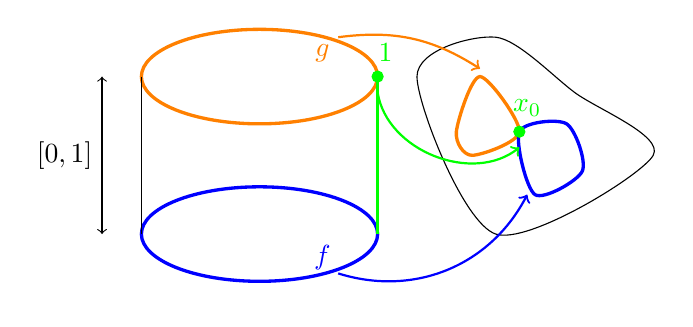
\begin{tikzpicture}
  \draw[orange, very thick] (-1, 1) ellipse (1.5 and 0.6);
  \draw[blue, very thick] (-1, -1) ellipse (1.5 and 0.6);

  \draw (-2.5, 1)--(-2.5, -1);
  \draw[green, very thick] (0.5, 1)--(0.5, -1);

  \filldraw[green] (0.5, 1) circle (2pt);
  \node at (0.6, 1.3) {$\color{green}1$};

  \draw[<->] (-3, 1)--(-3, -1) node [midway, left] {$[0,1]$};

  \draw[smooth cycle] plot coordinates {(1, 1) (2, 1.5) (3, 0.8) (4, 0) (2, -1)};
  \draw[smooth cycle, very thick, orange] plot coordinates {(2.3, 0.3) (1.8, 1) (1.5, 0.3) (1.7, 0)};
  \draw[smooth cycle, very thick, blue] plot coordinates {(2.3, 0.3) (2.9, 0.4) (3.1, -0.2) (2.5, -0.5)};
  \filldraw[green] (2.3, 0.3) circle (2pt);

  \node at (-0.2, 1.3) {$\color{orange}g$};
  \node at (-0.2, -1.3) {$\color{blue}f$};
  \node at (2.4, 0.6) {$\color{green}x_0$};

  \path[orange, thick, ->] (0, 1.5) edge[bend left=20] (1.8, 1.1);
  \path[blue, thick, ->] (0, -1.5) edge[bend right=40] (2.4, -0.5);
  \path[green, thick, ->] (0.5, 0.8) edge [bend right=60] (2.3, 0.1);
\end{tikzpicture}\end{center}

Grupa fundamentalna okręgu z wyróżnionym punktem jest izomorficzna z liczbami całkowitymi:
$$\Pi_1(S^1, 1)=\Z.$$

Mając dwie przestrzenie topologiczne $(X, x_0)$ i $(Y, y_0)$ oraz ciągłą funkcję między nimi $f$, mamy
\begin{center}\begin{tikzcd}[column sep=small, row sep=large]
  \Pi_1(X, x_0)\arrow[d, "\Pi_1(f)" left] & \left[\sigma\right] \arrow[l, phantom, sloped, "\ni"] \arrow[d, "\Pi_1(f)"] \\ 
  \Pi_1(Y, y_0) & \left[f\circ\sigma\right] \arrow[l, phantom, sloped, "\ni"]
\end{tikzcd}\end{center}

\end{example}

\begin{theorem}
  Każde ciągłe odwzorowanie $f:D^2\to D^2$ ma punkt stały.
\end{theorem}

\begin{proof}
  A raczej jego szkic.

  Załóżmy nie wprost, że istnieje funkcja ciągła $f:D^2\to D^2$, która nie posiada punktu stałego. 

  Możemy wówczas zdefiniować funkcję $F:D^2\to\partial D^2=S^1$, która punktowi $y\in D^2$ przypisuje punkt przecięcia wychodzącej z $f(y)$ przechodzącej przez $y$ z obwodem $D^2$:
  \begin{center}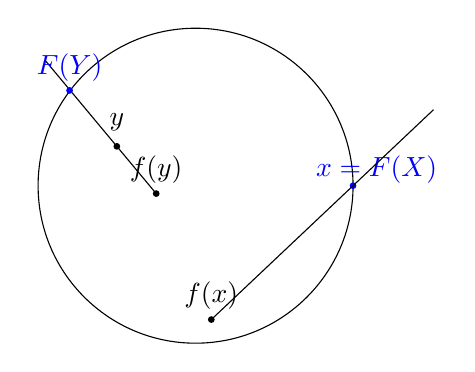
\begin{tikzpicture}
    \draw (0, 0) circle (2);

  \filldraw (-1, 0.5) circle (1pt);
  \node at (-1, 0.8) {$y$};

  \filldraw (-0.5, -0.1) circle (1pt);
  \node at (-0.5, 0.2) {$f(y)$};

  \draw[shorten <= -40pt] (-1, 0.5)--(-0.5, -0.1);
  \filldraw[blue] (-1.6, 1.21) circle (1pt);
  \node at (-1.6, 1.5) {$\color{blue}F(Y)$};


  \filldraw[blue] (2, 0) circle (1pt);
  \node at (2.3, 0.2) {$\color{blue}x=F(X)$};

  \filldraw (0.2, -1.7) circle (1pt);
  \node at (0.2, -1.4) {$f(x)$};

  \draw[shorten <= -40pt] (2, 0) -- (0.2, -1.7);
  \end{tikzpicture}\end{center}
  Obcięcie takiej funkcji do brzegu $\partial D^2$ daje oczywiście identyczność na $\partial D^2$ (punkt $x$ wyżej). Powstaje więc diagram
  \begin{center}\begin{tikzcd}
    S^1\arrow[rr, hookrightarrow]\arrow[dr, "id_{S^1}" below left] & & D^2 \arrow[dl, "F"] \\ 
                                  & S^1
  \end{tikzcd}\end{center}
  na który możemy nałożyć funktor $\Pi_1$:
  \begin{center}\begin{tikzcd}
    \Z=\Pi_1(S^1)\arrow[rr, hookrightarrow]\arrow[dr, "id_{\Z}=\Pi_1(id_{S^1})" below left] & & \Pi_1(D^2)=0 \arrow[dl, "\Pi_1(F)"] \\ 
                                  & \Pi_1(S^1)=\Z
  \end{tikzcd}\end{center}
  Czyli $\Z\to \Z$ faktoryzowałoby się przez $0$, a to jest niemożliwe.
\end{proof}

\begin{definition}[kategoria dualna]
  Dla kategorii $\mathbf{C}$ możemy zdefiniować nową kategorię, $\mathbf{C}^{op}$ w której każdy morfizm $\phi^{op}\in Hom_{\mathbf{C}^{op}}(Y, X)$ zostaje odwrócony:
  \begin{center}\begin{tikzcd}
    X\arrow[r, bend left=20, "\phi"] & Y\arrow[l, bend left=20, "\phi^{op}"]
  \end{tikzcd}\end{center}
  Wtedy $\ob\mathbf{C}^{op}$ to obiekty dualne do elementów znajdujących się w $\ob\mathbf{C}$. Tak zdefiniowaną kategorię $\mathbf{C}^{op}$ nazywamy \buff{kategorią dualną}.
\end{definition}

\begin{example}
\item Kategoria dualna do kategorii przestrzeni liniowych $\mathbf{Vect}_K^{op}$ jest kategorią, której obiekty to przestrzenie sprzężone, $V^*\in\ob\mathbf{Vect}^{op}_K$, zawierające funkcjonały liniowe $V\to K$. Każdy morfizm $\phi:V\to W$ w $\mathbf{Vect}_K$ indukuje wówczas odwzorowanie $\phi^*:W^*\to V^*$ takie, że dla $f\in W^*$ mamy $\phi^*(f)=f\circ\phi:V\to W\to K$.

  Kojarzenie funkcjonału $\phi^*\in V^*$ z elementem $v\in V$ jest czasem oznaczane przez $\langle \phi, v\rangle=\phi(v)$.
\end{example}

\begin{definition}[funktor kontrawariantny]
  Funktor (kowariantny) z kategorii $\mathbf{C}^{op}$ do kategorii $\mathbf{D}$ jest nazywamy \buff{funktorem kontrawariantnym} z $\mathbf{C}$ do $\mathbf{D}$.
\end{definition}

Oznacza to, że jeśli $X,Y\in\ob\mathbf{C}$ i $\phi:X\to Y\in Hom_{\mathbf{C}}(X, Y)$, to funktor kontrawariantny $F:\mathbf{C}^{op}\to\mathbf{D}$ przeprowadza $X$ na $F(X)\in\ob\mathbf{D}$, a $\phi\mapsto F(\phi)\in Hom_{\mathbf{D}}(F(Y),F(X))$.
\begin{center}\begin{tikzcd}[column sep=large]
  X \arrow[d, "\phi" left] \arrow[r, "F", yshift=-5mm, xshift=1mm, rightsquigarrow] & F(X) \\ 
  Y \arrow[d, "\psi" left] \arrow[r, "F", yshift=-5mm, xshift=1mm, rightsquigarrow] & F(Y) \arrow[u, "F(\phi)" right] \\ 
  Z & F(Z) \arrow[u, "F(\psi)" right] 
\end{tikzcd}\end{center}
Składanie morfizmów również zmienia kolejność, tzn.
$$F(\psi\phi)=F(\phi)F(\psi)$$









%Niech $R$ będzie dowolnym pierścieniem, natomiast $A, B, C$ będą $R$-modułami. Mając ciąg
%
%\begin{center}\begin{tikzcd}
%  A\arrow[r, "f"] & B\arrow[r, "g"] & C
%\end{tikzcd}\end{center}
%
%mówimy, że jest on \acc{dokładny}, jeśli $\ker(g)=\img(f)$. W szczególności implikuje to, że $g\circ f=gf:A\to C$ jest homomorfizmem zerowym.
%
%\begin{definition}[Kompleks łańcuchowy]
%  Rozważmy rodzinę $C=\{C_n\}_{n\in\Z}$ $R$-modułów wraz z mapami $d=d_n:C_n\to C_{n-1}$ takimi, że każde złożenie
%  $$[d_{n-1}\circ d_n=]d\circ d:C_n\to C_{n-2}$$
%  jest zerowe. Wówczas każdą mapę $d_n$ nazywamy \buff{różniczkami $C$}, a rodzina $C$ jest \buff{kompleksem łańcuchowym}.
%\end{definition}
%
%Jądra każdego $d_n$ nazywamy \acc{$n$-cyklami} $C$ i oznaczamy $Z_n=Z_n(C)$, natomiast obraz każdego $d_{n+1}$ jest nazywany \acc{$n$-granicą} $C$ i oznacza się jako $B_n=B_n(C)$. Ponieważ $d_n\circ d_{n+1}=0$, to
%$$0\subseteq B_n\subseteq Z_n\subseteq C_n.$$
%
%\begin{definition}[Homologia]
%  \buff{$n$-tym modułem homologii} kompleksu $C$ nazywamy iloraz $\color{green}H_n(C)=Z_n/B_n$.
%\end{definition}
%
%\begin{problem}
%  Ustalmy $C_n=\Z/8$ dla $n\geq0$ i $C_n=0$ dla $n<0$. Dla $n>0$ niech $d_n$ posyła $x\mod 8$ do $4x\mod 8$. Pokaż, że tak zdefiniowane $C$ jest kompleksem łańcuchowym $\Z/8$-modułów i policz moduły homologii.
%\end{problem}
%
%\begin{solution}
%  Zauważyć, że $d_{n-1}d_n=0$ jest nietrudno dla $n\leq1$ ($d_{n-1}d_n:C_n\to C_{n-2}=0$). Z kolei dla dowolnego $n>1$ i dowolnego $x\in C_n$ wiemy, że $d_n(x)=4x\mod 8$. Jeśli $x$ było oryginalnie liczbą parzystą, to od razu widać, że $d_n(x)=0$. Z kolei gdy $x$ jest nieparzyste, to wówczas 
%  $$d_{n-1}d_n(x)=d_{n-1}(4x\mod 8)=16x\mod 8=8\cdot(2x)\mod 8=0,$$
%  a więc $d_{n-1}d_n=0$.
%
%  Homologie dla $n<2$ są trywialne, natomiast dla $n\geq 2$ wszystkie są takie same (gdyż funkcje $d_n$ jak i moduły $C_n$ nie ulegają zmianie wraz z $n$). Wystarczy więc przyjrzeć się $Z_1/B_1$
%  
%  \begin{center}\begin{tikzcd}
%    C_0=\Z/8 & C_1=\Z/8\arrow[l, "d_1"] & C_2=\Z/8\arrow[l, "d_2"]
%  \end{tikzcd}\end{center}
%
%  $Z_1$ to liczby parzyste w $\Z/8$ (kernel $d_1$), natomiast $B_1$ to liczby podzielne przez $4$, ale nie przez $8$ w $C_1$. W takim razie, $Z_1/B_1=\{4\}$.
%\end{solution}

\newpage

\section{09.10.23 : Równoważność kategorii}

\subsection{Presnop i snop}

%\begin{definition}[Presnop]
  Niech $X$ będzie przestrzenią topologiczną i związaną z nią kategorię $\mathbf{Otw(X)}$ zdefiniujemy tak, że
  \begin{itemize}
    \item $\ob\mathbf{Otw(X)}=\{U\subseteq X\;:\;U\text{ - zbiór otwarty}\}$
    \item morfizmy to włożenia identycznościowe (tzn. istnieje morfizm $X\hookrightarrow Y$ jeśli $X\subseteq Y$)
  \end{itemize}

  Tak zdefiniowany funktor kontrawariantny $\mathbf{Otw(X)}^{op}\to \mathbf{C}$ nazywamy \buff{presnopem} na przestrzeni topologicznej $X$.
%\end{definition}

%Zamiast kategorii zbiorów $\mathbf{Set}$ możemy też mieć snop na kategorię grup abelowych, przestrzeni liniowych etc.
  Kategoria $\mathbf{C}$ może być kategorią zbiorów $\mathbf{Set}$, ale możemy też przeprowadzać zbiory otwarte oraz morfizmy między nimi na kategorię $\mathbf{Ab}$, $\mathbf{Vect}_K$ czy $R-\mathbf{mod}$. Wtedy taki funktor będziemy nazywać odpowiednio \acc{presnopem grup abelowych, przestrzeni liniowych czy $R$-modułów}.

\begin{example}
\item Zaczniemy od przetestowania presnopu na przestrzeni topologicznej w akcji.

  Niech $X$ będzie przestrzenią topologiczną, a $U\subseteq X$ będzie dowolnym zbiorem otwartym. Funktor $F:\mathbf{Otw(X)}^{op}\to {C(X)}$ definiujemy na obiektach jako
  $$F(U)=C(U)=\{f:U\to\C\;|\;f\text{ ciągła}\}$$
  Dla $V\subseteq U\subseteq X$ otwartych zbiorów mamy

  \begin{center}
    \begin{tikzcd}[row sep=tiny, column sep = large]
      F(U)\arrow[d, phantom, sloped, "="] & F(V)\arrow[l, "\text{obcięcie}" above]\arrow[d, phantom, sloped, "="]\\
      C(U) & C(V)\arrow[l]
    \end{tikzcd}
  \end{center}

  co w widoczny sposób spełnia $F(\phi\psi)=F(\phi)F(\psi)$.

  Funktor jak wyżej jest nazywany presnopem funkcji ciągłych.
\end{example}

\begin{definition}[presnop, snop]
  \buff{Presnopem} na kategorii $\mathbf{C}$ nazywamy dowolny funktor
  $$F:\mathbf{C}^{op}\to\mathbf{Set}$$

  \buff{Snopem} nazywamy presnop taki, że jeśli dla dowolnego zbioru $U=\bigcup_{i\in I}U_i$ oraz dla dowolnych $i,j\in I$ spełniony jest warunek
  $$s_i\restriction(U_i\cap U_j)=s_j\restriction(U_i\cap U_j),$$
  gdzie $s_i\in F(U_i)$ jest nazywane \acc{cięciem presnopu}, to wówczas istnieje dokładnie jedyne cięcie $s\in F(U)$ takie, że
  $$s\restriction U_i=s_i.$$
  Zapisując to za pomocą kwantyfikatorów mamy:
  \begin{align*}
    (\forall\;U=\bigcup_{i\in I}U_i)
    (\forall\;s_i\in F(U_i))\;
    &\left[ 
      (\forall i,j\in I)\;
      s_i\restriction(U_i\cap U_j)=s_j\restriction(U_i\cap U_j) 
    \right]
    \implies\\
    &\implies\left[
      (\exists!\;s\in F(U))
      (\forall i\in I)\;s\restriction U_i=s_i
    \right]
  \end{align*}
\end{definition}

\begin{example}
  \item Presnop na przestrzeni topologicznej $X$ spełnia również warunek opisany wyżej.
    %Przykład  z wcześniej spełnia również warunek bycia snopem. Tutaj wchodzą kiełki gromadzące się nad snopem i zbierające się w większe źdźbła, ale ja sobie to odpuszczę.
\end{example}

\subsection{Funktory wierne, pełne}

\begin{definition}[podkategoria $\mathbf{C}'$ kategorii $\mathbf{C}$]
  To kategoria spełniająca następujące warunki:
  \begin{itemize}
    \item $Ob\mathbf{C}'\subseteq Ob\mathbf{C}$
    \item $Hom_{\mathbf{C}'}(X,Y)\subseteq Hom_{\mathbf{C}}(X, Y)$
    \item $id_X^{\mathbf{C}'}=id_X^{\mathbf{C}}$ zawsze gdy $X\in Ob\mathbf{C}'$
    \item złożenie morfizmów w $\mathbf{C}'$ zachowuje się tak samo jak w $\mathbf{C}$
  \end{itemize}

  Mówimy, że podkategoria $\mathbf{C}'$ jest \acc{pełna}, gdy dla wszystkich $X,Y\in\ob\mathbb{C}'$ zachodzi $Hom_{\mathbf{C}'}(X,Y)=Hom_{\mathbf{C}}(X,Y)$
\end{definition}

\begin{example}
\item Kategoria przestrzeni skończonego wymiaru $\mathbf{Vect}_K^{fin}$ jest podkategorią kategorii wszystkich przestrzeni liniowych $\mathbf{Vect}_K$. Jest to pełna podkategoria.
\item Analogicznie, kategoria grup abelowych $\mathbf{Ab}$ jest pełną podkategorią kategorii $\mathbf{Grp}$
\item Kategoria gładkich rozmaitości $\mathbf{C^\infty-rozm}$ jest podkategorią kateogorii wszystkich przestrzeni topologicznych $\mathbf{Top}$. Nie jest to jednak pełna podkategoria.
\end{example}

\begin{definition}[funktor wierny, pełny]
  Funkctor $F:\mathbf{C}\to\mathbf{D}$ jest
  \begin{itemize}
    \item \buff{wierny} gdy $F:Hom_{\mathbf{C}}(X,Y)\to Hom_{\mathbf{D}}(F(X),F(Y))$ jest injekcją
    \item \buff{pełny}, gdy dla wszystkich $X,Y\in Ob\mathbf{C}$ przekształcenie $F:Hom_{\mathbf{C}}(X,Y)\to Hom_{\mathbf{D}}(F(X),F(Y))$ jest surjekcją
  \end{itemize}
\end{definition}

\begin{example}
\item Włożenie podkategorii w kategorię jest funktorem wiernym
\item Jeśli podkategoria jest pełna, to taki włożeniowy funktor jest dodatkowo pełny.
\end{example}

\subsection{Naturalne przekształcenia funktorów}

\begin{definition}[naturalne przekształcenie funktorów]
  Dla dwóch funktorów $F, G:\mathbf{C}\to\mathbf{D}$ układ morfizmów $f:F\to G$ w $\mathbf{D}$ taki, że dla każdego $X\in Ob\mathbf{C}$ $f(X):F(X)\to G(X)$ i dla każdego $\phi:X\to Y\in Hom_{\mathbf{C}}(X, Y)$ diagram

  $ $

  \begin{center}
    \begin{tikzcd}[column sep=large]
      F(X) \arrow[r, "f(X)"] \arrow[d, "F(\phi)" left] & G(X)\arrow[d, "G(\phi)"]\\
      F(Y) \arrow[r, "f(Y)" below] & G(Y)
    \end{tikzcd}
  \end{center}

  $ $

  jest przemienny nazywamy \buff{naturalnym przekształceniem funktorów} $F$ i $G$.
\end{definition}

\begin{example}
\item Patrzymy na funktory $Id, ab:\mathbf{Grp}\to\mathbf{Grp}$ (identyczność i abelianizacja $ab(G)=G/[G,G]$).

  Rozważmymy $f:Id\to ab$, wtedy $Id(G)=G$, więc sprawdzamy, czy następujący diagram komutuje:

  \begin{center}
    \begin{tikzcd}[column sep=large]
      Id(G)=G \arrow[r, "f(G)"] \arrow[d, "Id(\phi)=\phi" left] & G/\left[G, G\right] = ab(G) \arrow[d, "ab(\phi)"] \\
      Id(H)=H \arrow[r, "f(H)"] & H/\left[H, H\right] = ab(H)
    \end{tikzcd}
  \end{center}

  Dla każdego $G\in Ob\mathbf{Grp}$ zdefiniujemy $f(G):Id(G)\to ab(G)$ jako
  $$f(G):G\to G^{alb}=G/[G,G]$$
  jako zwykłe przekształcenie ilorazowe. Aby więc diagram komutował, czyli
  $$f(H)\circ Id(\phi)=ab(\phi)\circ f(G),$$ 
  wystarczy sprawdzić, że komutant grupy $G$ przechodzi przez dowolny homomorfizm na komutant w $H$:
  $$(\forall\;g,h\in [G,G])\;\phi(gh)=\phi(g)\phi(h)=\phi(h)\phi(g)=\phi(hg).$$
  Skoro tak jest, to nie ma znaczenia, czy najpierw abelianizujemy grupę, a potem nakładamy na to homomorfizm, czy najpierw nakładamy homomorfizm, a potem abelianizujemy.

%  \begin{center}
%    \begin{tikzcd}
%      Id(G)=G \arrow[r, "Id(\phi)"] \arrow[d, "f(G)"] & H=Id(H) \arrow[d]\\
%      \left[G, G\right] \arrow[r] & \left[H,H\right]
%    \end{tikzcd}
%  \end{center}
\item Można pokazać, że istnieje naturalne przekształcenie funktorów z kategorii przestrzeni topologicznych z wybranym punktem bazowym ($\mathbf{Top}_*$) w kategorię grup 
  $$H_n, \Pi_n:\mathbf{Top}_*\to\mathbf{Grp},$$
  gdzie $\Pi_n$ to funktor przypisujący przestrzeni $n$-tą homotopię ($\Pi_1$ w szczególności przyporządkowuje przestrzeni topologicznej jej grupę fundamentalną), a $H_n$ to funktor $n$-tej homologii.
  %Z odrobiną znajomości topologii algebraicznej możemy pokazać, że istnieje naturalne przekształcenie funktorów $H_n,\Pi_n:\mathbf{Top}_*\to\mathbf{Grp}$. Jednak nie znam się na topologii algebraicznej, więc ja tego nie zrobię.
  
\item Pokażemy naturalne przekształcenie funktorów $Id,\star\star:\mathbf{Vect}_K\to\mathbf{Vect}_K$.
  
  Dla $V\in\mathbf{Vect}_K$ definiujemy
  \begin{center}
    \begin{tikzcd}[column sep=large]%, row sep=tiny]
      f(V):V \arrow[r] & V^{**}\\
      v \arrow[u, phantom, sloped, "\in"] \arrow[r] & (V^*\ni\phi^*\mapsto\phi^*(v)\in K)=\langle\cdot,v\rangle \arrow[u, phantom, sloped, "\in"]
    \end{tikzcd}
  \end{center}
  to znaczy, dla $v\in V$ mamy element $f(V)(v)=\langle\cdot, v\rangle\in V^{**}$, który elementowi $\phi^*\in V^*$ przyporządkowuje $\langle\phi^*,v\rangle=\phi^*(v)\in K$.

  Chcemy sprawdzić, że diagram
  \begin{center}
    \begin{tikzcd}[column sep=large]
      V \arrow[r, "f(V)"] \arrow[d, "\phi" left] & V^{**} \arrow[d, "\phi^{**}"] \\
      W \arrow[r, "f(W)" below] & W^{**}
    \end{tikzcd}
  \end{center}
  komutuje, czyli pokazać, że $f(V)\circ\phi^{**}=\phi\circ f(W)$.
  
  Troszkę przypomnienia z algebry liniowej. Przekształcenie liniowe $\phi:V\to W$ indukuje funkcjonał liniowy $\phi^*:W^*\to V^*$ taki, że dla $f:W\to K\in W^*$ mamy $\phi^*(f)=f\circ \phi\in V^*$. W takim razie, przekształcenie $\phi^{**}:V^{**}\to W^{**}$ dla $f^*:V^{*}\to K\in V^{**}$ przyporządkuje
  $$\phi^{**}(f^*)=f^*\circ\phi^*:W^*\to K$$
  \begin{align*}
    (\phi^{**}\circ f(V))(v)&=\phi^{**}(f(V)(v))=\phi^{**}(\langle\cdot,v\rangle)=\\
                            &=\langle\cdot,v\rangle\circ\phi^*=\langle\phi^*(\cdot),v\rangle=\\
                            &=\langle \cdot\circ\phi,v\rangle=\langle\cdot,\phi(v)\rangle=f(W)(\phi(v))=\\
                            &=(f(W)\circ\phi)(v)
  \end{align*}
  element $W^{**}$.

  Czyli wszystko się zgadza!
\end{example}

Naturalne przekształcenia można składać. Powstaje wtedy (meta)kategoria, której elementy to funktory, a morfizmami są naturalne przejścia. Nie jest to prawdziwa kategoria, bo morfizmy nie zawsze tworzą zbiory w takim przypadku. Taki twór oznaczamy $\color{blue}\mathbf{Funct}(\mathbf{C},\mathbf{D})$ i mając naturalne przekształcenia funktorów $F\overset{a}{\to} G\overset{b}{\to}H$, dowolne $X,Y\in Ob\mathbf{C}$ oraz $\phi:X\to Y$ rysujemy
\begin{center}
  \begin{tikzcd}[column sep=large]
    F(X) \arrow[r, "a(X)"] \arrow[d, "F(\phi)" left] & G(X) \arrow[r, "b(X)"] \arrow[d, "G(\phi)"] & H(X) \arrow[d, "H(\phi)"] \\
    F(Y) \arrow[r, "a(Y)" below] & G(Y) \arrow[r, "b(Y)" below] & H(Y)
  \end{tikzcd}
\end{center}
gdzie $(b\circ a)(X)=b(X)\circ a(X)$.

\begin{definition}[izomorfizm funktorów]
  W metakategorii funktorów możemy rozważać izomorfizmy, które nazywamy \buff{naturalnymi izomorfizmami funktorów}. Do ich definiowania można podejść na dwa, równoważne, sposoby:
  \begin{itemize}
    \item naturalne przekształcenia $f:F\to G$ dla których istnieje $g:G\to F$ takie, że $f\circ g=id_G$ oraz $g\circ f=id_F$
    \item przekształcenie $f:F\to G$ takie, że dla każdego $X\in\mathbf{C}$ przekształcenie $f(X):F(X)\to G(X)$ jest izomorfizmem w kategorii $\mathbf{D}$.
  \end{itemize}
\end{definition}

\begin{example}
  \item Przekształcenie funktorów $Id, **$ na kategorii przestrzeni wektorowych rozważane wyżej staje się izomorfizmem, gdy ograniczymy się do przestrzeni skończonego wymiaru.
\end{example}

\subsection{Równoważność kategorii}

\begin{definition}[równoważność kategorii]
  Funktor $F:\mathbf{C}\to\mathbf{D}$ zadaje \buff{równoważność kategorii}, jeśli istnieje funktor $G:\mathbf{D}\to\mathbf{C}$ oraz naturalne przekształcenia funktorów $f:F\circ G\to Id_{\mathbf{D}}$ i $g:G\circ F\to Id_{\mathbf{C}}$
\end{definition}

Równoważność kategorii jest nieco słabszym warunkiem niż istnienie izomorfizmu między nimi - złożenie $F\circ G$ niekoniecznie musi być równe $Id_{\mathbf{D}}$, wystarczy tylko żeby istniało naturalne przekształcenie między tymi dwoma funktorami.

\begin{example}
\item Kategoria skończenie wymiarowych przestrzeni wektorowych $\mathbf{Vect}_K^{fin}$ jest równoważna kategorii $\mathbf{S_K}$, której obiektami są $Ob\mathbf{S_K}=\{K^0,K^1,...,K^n,...\}$ a morfizmy to wszystkie przekształcenia liniowe między nimi.

  Funktor włożenia
  $$F:\mathbf{S_K}\to \mathbf{Vect}_K^{fin}$$
  jest oczywistym wyborem na pierwszy funktor, gdyż każdy obiekt z $\mathbf{S_K}$ jest przestrzenią wektorową skończonego wymiaru.

  Aby znaleźć funktor
  $$G:\mathbf{Vect}_K^{fin}\to\mathbf{S_K}$$
  zaczniemy od rozważenia na co przechodzi $V\in\mathbf{Vect}_K^{fin}$. Wiemy, że $\dim\mathbf{Vect}_K^{fin}=\infty$, możemy więc zdefiniować
  $$G(V)=K^{\dim\mathbf{Vect}_K^{fin}}.$$
  Pozostaje zastanowić się nad przekształceniem morfizmów. W każdym $V$ możemy wyróżnić pewną bazę, a każde przekształcenie liniowe $V\to W$ będzie macierzą o wyrazach w $K$ zapisaną w tych wyróżnionych bazach. Wystarczy więc przekształceniu $V\to W$ zadanemu macierzą przyporządkować przekształcenie wyznaczone przez taką samą macierz na $K^{\dim V}\to K^{\dim W}$.

\end{example}

\begin{theorem}
  Funktor $F:\mathbf{C}\to \mathbf{D}$ zadaje równoważność kategorii $\iff$ jest on wierny, pełny i w zasadzie surjektywny, tzn. $(\forall\;Y\in \ob\mathbf{D})(\exists\;X\in \ob\mathbf{C})\;F(X)\underset{\mathbf{D}}{\cong}Y$.
\end{theorem}

\begin{proof}
  $\impliedby$

  Wiemy, że funktor $F:\mathbf{C}\to\mathbf{D}$ jest wierny, pełny i w zasadzie suriektywny i na podstawie tej wiedzy skonstruujemy $G:\mathbf{D}\to\mathbf{C}$ jak w definicji równoważności kategorii.

  Dla $Y\in \ob\mathbf{D}$ wybieramy $G(Y)\in \ob\mathbf{C}$ takie, że istnieje izomorfizm $\iota_Y:Y\to F(G(Y))$. Możemy tak zrobić, gdyż $F$ jest w zasadzie suriektywny. 

  Niech $\phi:Y\to Y'$ będzie morfizmem obiektów w kategorii $\mathbf{D}$. Chcemy sprawdzić istnienie $G(\phi)$ takie, że mamy naturalny izomorfizm $Id_{\mathbf{D}}\leftrightarrow F\circ G$

  \begin{center}
    \begin{tikzcd}[column sep=large]
      Id_{\mathbf{D}}(Y)=Y \arrow[r, "\phi"] \arrow[d, "\iota_Y" left] & Y'=Id_{\mathbf{D}}(Y') \arrow[d, "\iota_{Y'}"]\\
      F(G(Y)) \arrow[r, "F(G(\phi))?" below] & F(G(Y'))
      %\iota_{Y'}\circ\phi\circ\iota_Y^{-1}" below ] & F(G(Y'))
    \end{tikzcd}
  \end{center}

  Ponieważ $\iota_Y$ jest izomorfizmem, dolną strzałkę $F(G(Y))\to F(G(Y'))$ możemy podpisać jako $\iota_{Y'}\circ\phi\circ\iota_Y^{-1}$. Chcemy pokazać, że da się dobrać $G(\phi)$ tak, żeby $F(G(\phi))=\iota_{Y'}\circ\phi\circ\iota_Y^{-1}$, tzn. żeby diagram na górze komutował.

  $F$ jest wierny i pełny, więc przejście
  $$Hom_{\mathbf{C}}(G(Y),G(Y'))\overset{F}{\rightarrow}Hom_{\mathbf{D}}(F(G(Y)),F(G(Y')))$$
  jest jednocześnie bijekcją i inijekcją, czyli możemy je odwracać. Istnieje więc jedyne 
  $$\psi=F^{-1}(\iota_{Y'}\phi\iota_Y^{-1}):G(Y)\to G(Y')$$
  które możemy przypisać do $G(\phi)=\psi$. Zbiór izomorfizmów $\iota_Y$ zadaje więc naturalny izomorfizm $Id_{\mathbf{D}}\to F\circ G$:
  \begin{center}\begin{tikzcd}[column sep=3cm, row sep=large]
    Y \arrow[d, "\iota_Y" left] \arrow[r, "\phi"] & Y' \arrow[d, "\iota_{Y'}"] \\ 
    F(G(Y)) \arrow[r, "F(G(\phi))=F(\psi)=\iota_{Y'}\phi\iota_Y^{-1}" below] & F(G(Y'))
  \end{tikzcd}\end{center}

  Pozostaje sprawdzić, że dla tak zdefiniowanego $G$ istnieje również naturalne przekształcenie $Id_{\mathbf{C}}\to G\circ F$.

  Dla $X, X'\in\ob\mathbf{C}$ oraz $\psi:X\to X'$ istnieje izomorfizm $F(X)\cong F(G(F(X)))$, gdyż tak właśnie zdefiniowaliśmy funktor $G$. Aby utrzymać konwencję z powyższego fragmentu dowodu, naziwjmy te izomorfizmy odpowiednio $\iota_{F(X)}$ i $\iota_{F(X')}$:
  \begin{center}\begin{tikzcd}
    F(X)\arrow[r, "\iota_{F(X)}"] \arrow[d, "F(\psi)" left] & F(G(F(X))) \arrow[d, "F(G(F(\psi)))"] \\ 
    F(X') \arrow[r, "\iota_{F(X')}" below] & F(G(F(X')))
  \end{tikzcd}\end{center}
  Ponieważ $F$ jest wiernym i pełnym funktorem, to możemy najbardziej zewnętrzne $F$ zdjąć, by otrzymać diagram:
  \begin{center}\begin{tikzcd}[column sep=large]
    X\arrow[r, "F^{-1}(\iota_{F(X)})"] \arrow[d, "\psi" left] & G(F(X)) \arrow[d, "G(F(\psi))"] \\ 
    X' \arrow[r, "F^{-1}(\iota_{F(X')})" below] & G(F(X'))
  \end{tikzcd}\end{center}
  Ponieważ diagram przed zdjęciem $F$ był przemienny, to również diagram niżej musi taki być - w końcu to zwykłe nałożenie $F^{-1}$ na wszystkie elementy i strzałki. W takim razie, morfizmy $F^{-1}(\iota_{F(X)})$ zadają naturalny izomorfizm $Id_{\mathbf{C}}\to G\circ F$.

  $\implies$

  Dowód drugiej implikacji zostaje pozostawiony jako ćwiczenie.
\end{proof}

\newpage

\section{16.10.2023 : Funktory reprezentowalne i granice}

\subsection{Kategoria funktorów}

W kategorii $\mathbf{Set}$ zbiór $X\in \ob\mathbf{Set}$ możemy widzieć jako $Hom_{\mathbf{Set}}(1,X)$ gdzie $1$ jest singletonem. Robimy to utożsamiając element $x\in X$ z morfizmem $1\mapsto x\in Hom_{\mathbf{Set}}(1, X)$.

Uogólniając obserwację wyżej, w dowolnej kategorii $\mathbf{C}$ obiektowi $X$ możemy przypisać funktor 
    $$h_X:\mathbf{C}^{op}\to \mathbf{Set}$$
    $$h_X(Y)=Hom_{\mathbf{C}}(Y, X) \; (\star)$$
    gdzie $(\star)$ zapisujemy czasem jako $X(Y)$.

    Ponieważ nie we wszystkich kategoriach istnieje odpowiednich singletona $1$, musimy rozważać wszystkie obiekty $Y$ i morfizmy:
    
    \begin{center}\begin{tikzcd}[column sep = large]
      %Y \arrow[r, "f"] & Y' \arrow[r, rightsquigarrow] & h_X(Y') \arrow[r, "h_X(f)"] & h_X(Y')
      Y \arrow[r, "f"] \arrow[d, "\alpha" left] & Y' \arrow[d, "\alpha\circ f"] \\
      X \arrow[r, squiggly, no head, "h_X(f)" below] & X
    \end{tikzcd}\end{center}
    dobrane tak, że diagram komutuje.

    %Tutaj równanie $(\star)$ można również zapisać jako $X(Y)$, czyli rozumieć jako $Y$-punkty obiektu $X$.

    Oczywiście, możemy też definiować funktor kowariantny $g:\mathbf{C}\to\mathbf{Set}$ taki, że $g_X(Y)=Hom_{\mathbf{C}}(X, Y)$.

\begin{definition}[Kategoria funktorów i funktory reprezentowalne]
  \acc{Kategorię funktorów} $(C^{op},\mathbf{Set})$, której obiektami są $h_X$ jak w przykładzie wyżej, oznaczamy $\hat{\mathbf{C}}$. 

  Funktor $F\in\hat{\mathbf{C}}$ jest \buff{reprezentowalny}, jeśli $F\cong h_X$ dla pewnego $X\in Ob\mathbf{C}$. Takie $X$ jest jedyne z dokładnością do izomorfizmu.
 
  Dla morfizmu $X\xrightarrow{\phi} X'$ w $\mathbf{C}$ określamy morfizm $h_\phi:h_X\to h_{X'}$ w $\mathbf{\hat{C}}$.

  \begin{center}\begin{tikzcd}[column sep=large, row sep = small]
    Hom_{\mathbf{C}}(Y,X) \arrow[r, "h_\phi"] & Hom_{\mathbf{C}}(Y,X')\\
    \alpha\arrow[u, phantom, sloped, "\in"] \arrow[r] & \phi\circ\alpha\arrow[u, phantom, sloped, "\in"]
  \end{tikzcd}\end{center}
\end{definition}

Funktor $h_X$ można również oznaczyć jako $Hom_{\mathbf{C}}(-, X)$. Wówczas dla morfizmu $\phi:Y\to Y'$ mamy 
$$h_\phi(\alpha)=Hom_{\mathbf{C}}(\phi, X)(\alpha)=\phi\circ\alpha$$
dla $\alpha\in Hom_{\mathbf{C}}(-, X)$

\begin{example}
  \item $\set{P}(X):\mathbf{Set}\to\mathbf{Set}$ jest funktorem, który przypisuje $X$ jest zbiór potęgowy. Jest on reprezentowalny, bo $\set{P}(X)\cong Hom(X, 2)$.
    
    Dla dowolnego zbioru $X\in\mathbf{Set}$ naturalne przekształcenie $f(X):Hom(X, 2)\to \set{P}(X)$ przypisze funkcji $\alpha\in Hom(X, 2)$ zbiór tych elementów $x\in X$ dla których $\alpha(x) = 2$. Przekształcenie odwrotne do tego przypisze zbiorowi $A\in\set{P}(X)$ funkcję $\alpha:X\to 2$ taką, że $\alpha(x)=1$ jeśli $x\notin A$ i $\alpha(x)=2$ wpp.

  \item Funktor kohomologii $H^n:\mathbf{C}\to\mathbf{Ab}$ z kategorii $CW$-kompleksów w grupy abelowe taki, że $H^n(X,G)=[X,K(G, n)]$ jest funktorem reprezentowalnym. Pokazuje to twierdzenie Browna o reprezentowalności o którym uczy się przy okazji topologii algebraicznej.
    %\emph{\large\color{red}NIE JESTEM PEWNA CO TO OZNACZA? chyba nie homotopie}
  
  \item {\large\color{red}co tutaj mają do roboty wiązki styczne?} $Vect_n(X)=[X,C^\infty]$????
\end{example}

Przyporządkowania $X\mapsto h_X$ oraz $\phi\mapsto h_\phi$ dają w oczywisty sposób funktor $h:\mathbf{C}\to\mathbf{\hat{C}}$.

\begin{lemma}[Yoneda lemma]
  Przyporządkowanie $h:\mathbf{C}\to\mathbf{\hat{C}}$ zadaje równoważność kategorii $\mathbf{C}$ z pełną podkategorią kategorii $\mathbf{\hat{C}}$, której obiektami są funktory reprezentowalne.
\end{lemma}

\begin{proof}
  Wystarczy pokazać, że $h$ jest funktorem wiernym, pełnym i w zasadzie surjektywnym.

  \begin{center}\begin{tikzcd}[column sep=large]
    X\arrow[d, "\phi" left]\arrow[r, "h(X)"] & h_X=Hom_{\mathbf{C}}(-, X)\arrow[d, "h_\phi"]\\ 
    X'\arrow[r, "h(X')"] & h_{X'}=Hom_{\mathbf{C}}(-, X')
  \end{tikzcd}\end{center}

  Chcemy pokazać, że przekształcenie $h$
  \begin{center}\begin{tikzcd}[column sep=large]
    Hom_{\mathbf{C}}(X, X')\arrow[r] & Hom_{\hat{\mathbf{C}}}(h_X, h_{X'})\\ 
    \phi\arrow[r, blue, "h"]\arrow[u, phantom, sloped, "\in"] & h_\phi\arrow[u, phantom, sloped, "\in"]
  \end{tikzcd}\end{center}
  jest bijekcją.




  Musimy pokazać, że

  \begin{center}\begin{tikzcd}[column sep=large, row sep=small]
    Hom_{\mathbf{C}}(X, X')\arrow[r, "\sim"] & Hom_{\mathbf{\hat{C}}}(h_X, h_{X'})\\
    \phi\arrow[u, phantom, sloped, "\in"]\arrow[r] & h_\phi\arrow[u, phantom, sloped, "\in"]
  \end{tikzcd}\end{center}

  jest bijekcją.
  
  Jeśli funktor $F\in\mathbf{\hat{C}}$ jest reprezentowalny, to reprezentujący go obiekt jest jedyny z dokładnością do izomorfizmu, bo

  \begin{center}\begin{tikzcd}
    & F\arrow[dr, "\cong"] \arrow[dl, "\cong" left]\\
    h_X\arrow[rr, rightsquigarrow, "\star\star", bend left=20] & & h_{X'}\\
    X\arrow[rr, "\star"] & & X'
  \end{tikzcd}\end{center}

  izomorfizm $\star$ pojawia się bezpośrednio po tym, że $F\to h_X$ i $F\to h_{X'}$ są izmorfizmami z definicji i od razu zadają izomorfizm $\star\star$.

  Niech teraz $F\in Hom_{\mathbf{\hat{C}}}(h_X,h_{X'})$.

  Jeśli $F=h_{\mathbf{C}}$, to mamy
  \begin{center}\begin{tikzcd}[column sep=large]
     h_X(X)\ni id_X\arrow[r, bend left=30, "h_\phi"]\arrow[r, bend right=30, "f"] & h_{X'}(X)
  \end{tikzcd}\end{center}

  {\large\color{red}WRÓCIĆ TUTAJ BO NIE WIEM CO SIĘ DZIEJE}

\end{proof}

\subsection{Granice i kogranice}

Czyli o granicach odwrotnych [granica] i prostych [kogranica].

\begin{definition}[system prosty i odwrotny]
  Niech $\mathbf{C}$ będzie kategorią, a $I$ zbiorem uporządkowanym. Układ $\{X_i, h_{ij}\}$ obiektów $\mathbf{C}$, gdzie dla $i\leq j$ $h_{ij}:X_i\to X_j$ są morfizmami w $\mathbf{C}$, nazywamy \buff{systemem prostym}, jeżeli
  \begin{enumerate}
    \item dla każdego $i\in I$ mamy $h_{ii}=id_{X_i}$
    \item jeśli $i\leq j\leq k$, to komutuje następujący diagram
      \begin{center}\begin{tikzcd}
        X_i\arrow[r, "h_{ij}"] \arrow[dr, "h_{ik}" below left] & X_j\arrow[d, "h_{jk}"] \\ 
                                                    & X_k
      \end{tikzcd}\end{center}
  \end{enumerate}

  Jeżeli z kolei mamy układ spełniający warunek 1, ale zamiast diagramu w warunku 2. komutuje diagram
  \begin{center}\begin{tikzcd}
    X_k\arrow[r, "h_{jk}"]\arrow[dr, "h_{ik}" below left] & X_j \arrow[d, "h_{ij}"] \\ 
                                                         & X_i
  \end{tikzcd}\end{center}
  to taki układ nazywamy \buff{systemem odwrotnym}
\end{definition}

Niech $I$ będzie małą kategorią, a $F:I\to\mathbf{C}$ będzie funktorem.

\begin{definition}[granica funktora $F$]
  Obiekt $X$ z rodziną odwzorowań (zbioru morfizmów) $\Pi_i:X\to F(i)$ dla $X\in Ob\mathbf{C}$ , które spełniają
  \begin{itemize}
    \item \acc{[zgodność]} dla dowolnych $i\xrightarrow{\alpha}j$ w $I$ diagram
      \begin{center}\begin{tikzcd}
        & X\arrow[dl, "\Pi_i" above left]\arrow[dr, "\Pi_j"]\\
        F(i)\arrow[rr, "F(\alpha)" below] & & F(j)
      \end{tikzcd}\end{center}
      komutuje, tzn. $\Pi_j=F(\alpha)\circ\Pi_i$.
    \item \acc{[uniwersalność]} dla każdego układu $(X',\Pi_i')$ spełniającego poprzedni warunek istnieje jedyny morfizm $\lambda:X'\to X$ taki, że dla każdego $i\in I$ diagram
      \begin{center}\begin{tikzcd}
      X'\arrow[rr, "\exists!\lambda"]\arrow[dr, "\Pi_i'" below left] & & X\arrow[dl, "\Pi_i"]\\
      & F(i)
    \end{tikzcd}\end{center}
    komutuje
  \end{itemize}
  jest nazywany \buff{granicą funktora $F$} i oznaczamy ją jako $\lim F$.
\end{definition}

Granica funktora może nie istnieć, ale zawsze gdy istnieje, to jest jedyna z dokładnością do izomorfizmu.

\begin{example}
  \item Dla $I=\{0,1\}$ oraz $F:I\to \mathbf{C}$ granicę $\lim F$ nazywamy \acc{produktem} obiektów $F(0)$ i $F(1)$
    \begin{center}\begin{tikzcd}[column sep=large]
      X\arrow[r, "\Pi_1"]\arrow[d, "\Pi_0" left]\arrow[dr, dashed] & F(1)\\
      F(0) & X'\arrow[l, "\Pi_0'"]\arrow[u, "\Pi_1'" right]
    \end{tikzcd}\end{center}
\end{example}

\begin{definition}[granica odwrotna]
  \begin{center}\begin{tikzcd}
  \end{tikzcd}\end{center}
\end{definition}

\newpage

\section{23.10.23 : Kategorie abelowe i addytywne, jądra}

\subsection{Funktory sprzężone [adjoint functors]}


\begin{definition}[funktory sprzężone]
  Para funktorów $L:\mathbf{A}\to\mathbf{B}$ i $R:\mathbf{B}\to\mathbf{A}$ nazywamy \buff{parą sprzężoną} ($L$ jest lewo sprzężony do $R$, a $R$ jest prawo sprzężony do $L$), jeśli istnieją naturalne bijekcje (zarówno względem $\mathbf{A}$ jak i $\mathbf{B}$)
  $$Hom_{\mathbf{B}}(L(A),B)\longleftrightarrow Hom_{\mathbf{A}}(A,R(B))$$

  Funktory sprzężone oznaczamy $L\dashv R$
\end{definition}

\begin{example}
  \item Jest sporo przykładów, gdy $R$ jest \acc{funktorem zapominającym}
    \begin{itemize}
      \item jeśli $R:\mathbf{Grp}\to\mathbf{Set}$, wtedy

        \begin{center}\begin{tikzcd}[row sep=tiny]
          Hom_{\mathbf{Grp}}(\star,B)\arrow[r, <->] & Hom_{\mathbf{Set}}(A,B)\\
          \text{grupa}\arrow[u, start anchor={[yshift=-2mm, xshift=3mm]}, end anchor={[xshift=5mm, yshift=2mm]}, bend right=30] & &\text{grupa jako zbiór}\arrow[ul, start anchor={[xshift=1mm]west}, end anchor={[xshift=4mm, yshift=1mm]}, bend left=15]
        \end{tikzcd}\end{center}

        $\star$ będzie grupą wolną o zbiorze generatorów $A$, co oznaczamy $F_A$.
      \item $R:\mathbf{Vect}_K\to\mathbf{Set}$ z bijekcjami zdefiniowanymi jako
        $$Hom_{\mathbf{Vect}_K}(LA,V)\longleftrightarrow Hom_{\mathbf{Set}}(A,V)$$
        gdzie $LA$ to przestrzeń liniowa o bazie równej zbiorowi $A$.
    \end{itemize}
  \item Dla $R$-modułów $A,B,X$ zachodzi
        $$Hom_R(A\otimes X, B)\cong Hom_R(A,Hom_R(X,B))$$
        dla $\phi\in Hom_R(A,Hom_R(X,B))$ mamy
        $$(a\otimes x\mapsto (\phi(a))(x))\mapsto \phi$$
        Dla ustalonego $X$ mamy funktory sprzężone z $R$-modułów w $R$-moduły: $L=-\otimes X$ oraz $R=Hom(X,-)$
  \item Bardzo często włożenie kategorii w inną kategorię jest funktorem mającym funktor sprzężonym.
    \begin{itemize}
      \item Włożenie kategorii $\mathbf{Ab}\hookrightarrow \mathbf{Grp}$ posiada funktor sprzężony:
      $$Hom_{\mathbf{Ab}}(\star, B)\longleftrightarrow Hom_{\mathbf{Grp}}(A, B)$$
      komutant dowolnej grupy $A$ przechodzi przez każdy homomorfizm $\phi:A\to B$ na element neutralny, więc od razu indukwoane mamy przekształcenie $A^{op}\to B$, stąd $\star=A^{op}$.
    \item Włożenie kategorii ciał w dziedziny wyrzuca część homomorfizmów. Mamy
      $$Hom_{\mathbf{Ciala}}(\star,K)\longleftrightarrow Hom_{\mathbf{Dziedziny}}(R,K)$$
      Jeśli mamy odwzorowanie z pierścienia $R$ w ciało $K$, to to odwzorowanie rozszerza się na odwzorowanie z ciała ułamków ciała $R$ w ciało $K$:
  
      \begin{center}\begin{tikzcd}
        R\arrow[rr, "\phi"]\arrow[dr, hookrightarrow] & & K\ni\frac{\phi(p)}{\phi(q)}\\
         & R_0\ni \frac{p}{q}\arrow[ur]
      \end{tikzcd}\end{center}
  
      stąd $\star=R_o$
    \item Włożenie zwartych przestrzeni Hausdorffa w przestrzenie topologiczne $\mathbf{Cpt}T_0\hookrightarrow \mathbf{Top}$ mamy
      $$Hom_{\mathbf{Cpf}T_0}(\star, Y)\longleftrightarrow Hom_{\mathbf{Top}}(X,Y)$$
      więc $\star=\beta X$ czyli uzwarceniem Cecha-Stone'a. To jest maksymalne możliwe uzwarcenie. 
  
      Bierzemy przestrzeń $X$ i patrzymy na wszystkie ciągłe odwzorowania z $X$ w $[0,1]$ i potem odwzorowujemy diagonalnie $X$ w ten produkt, a potem domykamy obraz tego diagonalnego odwzorowania i to jest maksymalne uzwarcenie.
  \end{itemize}
\end{example}

\begin{fact}[jedyność funktora sprzężonego]
  Funktor sprzężony, jeśli istnieje, to jest jedyny z dokładnością do izomorfizmu.
\end{fact}

\begin{proof}
  Bardzo poglądowy, bo trzeba się dokładnie wgryźć w spojrzenie jak to działa na morfizmach.

  $R(B)$ to jedyny element reprezentujący funktor
  $$A^{op}\ni A\mapsto Hom_{\mathbf{B}}(LA,B)\in\mathbf{Set}$$
    Z lematu Yonedy wiemy, że jeśli takie coś istnieje, to jest jedyne z dokładnością do izomorfizmu.
\end{proof}

\begin{fact}[funktory sprzężone zachowują granice (prostą/odwrotną)]\label{funktory sprzezone zachowuja granice}
  Jeśli $L\dashv R$, to $R$ zachowuje granicę, a $L$ kogranicę.
\end{fact}

\begin{proof}
  {\large\color{red}OBRAZEK}

  Musimy wziąć dowolny obiekt $A\in \mathbf{A}$ i sprawdzić, czy $\Pi_i':A\to (R\circ F)(I)$ sfaktoryzuje się w jedyny możliwy sposób na $R\circ R(\Pi_i)$. Musimy wziąć obiekt $LA\in\mathbf{B}$ i tutaj dostajemy jedyną strzałkę $LA\to X$, gdyż $X$ jest granicą. Ale sprzężoność $R$ z $L$ mówi, że mamy jedyność odpowiadania strzałek między elementami $\mathbf{A}$ a elementami $\mathbf{B}$.
\end{proof}

\subsection{Kategorie addytywne i abelowe}

\begin{definition}[kategoria addytywna]
  \buff{Kategoria addytywna} $\mathbf{A}$ to kategoria
  \begin{itemize}
    \item Dla każdej pary obiektów $A,B\in Ob\mathbf{A}$ na $Hom_{\mathbf{A}}(A, B)$ jest określona struktura grupy abelowej. Złożenia są biaddytywne:
      \begin{center}\begin{tikzcd}
        A\arrow[r, "g"] & B\arrow[r, "f", bend left=10]\arrow[r, "f'", bend right=10] & C\arrow[r, "h"] & D
      \end{tikzcd}\end{center}
      $$(f+f')\circ g=f\circ g+f'\circ g$$
      $$h\circ(f+f')=h\circ f+h\circ f'$$
    \item Istnieje \acc{obiekt zerowy} $0$ taki, że $Hom_{\mathbf{A}}(0, 0)=0$ jest grupą trywialną
    \item Dla dowolnej pary obiektów $A, B\in Ob\mathbf{A}$ istnieje obiekt $C$ (zwykle oznaczany $A\oplus B$), który jest ich \acc{produktem} i \acc{koproduktem}, tzn.: istnieją morfizmy
      \begin{center}\begin{tikzcd}
        A\arrow[r, "i_A"] & C\arrow[l, "P_A"]\arrow[r, "P_B"] & B\arrow[l, "i_B"]
      \end{tikzcd}\end{center}
      takie, że $P_a\circ i_A=id_A$ i $P_A\circ i_B=0$ (analogicznie gdy przestawimy $A$ i $B$). Dodatkowo, $i_AP_A+i_BP_B=id_C$.
  \end{itemize}
\end{definition}

Tłumacząc ostatni warunek, chcemy pokazać, że istnieje jedyna strałka $D\to C$:
\begin{center}\begin{tikzcd}
  D\arrow[dr, dashed]\arrow[drr, bend left=20, "f_b"]\arrow[ddr, "f_A", bend right=20] & &\\
                                                       & C\arrow[r, "P_B"]\arrow[d, "P_A"] & B\\
                                                       & A
\end{tikzcd}\end{center}
Zauważmy że $i_Af_A+i_Bf_B:D\to C$, wystarczy więc sprawdzić, czy taka definicja $D\to C$ sprawia, że diagram komutuje, tzn. złożyć ją z $P_A$ i $P_B$:
%({\large\color{red}TUTAJ ZDJĘCIE Z MNÓSTWEM OBLICZEŃ})
$$P_A(i_Af_A+i_Bf_B)=\underbrace{P_Ai_A}_{id_A}f_A+\underbrace{P_Ai_B}_{0}f_B=f_A$$
$$P_B(i_Af_A+i_Bf_B)=\underbrace{P_Bi_A}_{0}f_A+\underbrace{P_Bi_B}_{id_B}f_B=f_B$$
Jeśli istnieją dwa takie odwzorowania, to ich różnica $u$ zamykałaby diagram
\begin{center}\begin{tikzcd}
  D\arrow[drr, "0", bend left=20]\arrow[ddr, "0", bend right=20]\arrow[dr, "u"]\\
  & C\arrow[r, "P_B"]\arrow[d, "f_A"] & B\\
  & A
\end{tikzcd}\end{center}Zauważmy, że 
\begin{align*}
  u&=id_C\circ 0=\\
   &=i_AP_Au+i_BP_Bu=\\
   &=i_A0+i_B0=0+0=0
\end{align*}

Analogicznie pokazuje się dla koproduktu.

\begin{dygresja}[parę słów o zerach]
  Dla dowolnego obiektu $A\in Ob\mathbf{A}$ mamy $Hom(0, A)=0$ i $Hom(0, A)=0$, bo dla $f:A\to 0$ jest $id_0\circ f=f$, czyli $f=0\circ f$, a więc
  $$0f=(0+0)f=0f+0f\implies 0=0f\implies f=0$$
\end{dygresja}

\begin{example}
\item $\mathbf{AB}$
\item $R$-moduły
\item Presnopy grup abelowych na jakiejś przestrzeni topologicznej (lub kategorii) 

  $\mathbf{Pre-snop/AB}(X)$ i od razu zagubione w tym gąszczu snopy.
\end{example}

\begin{definition}[kategoria abelowa]
  Kategoria addytywna jest \buff{abelowa}, jeśli każdy morfizm ma jądro i kojądro i naturalny morfizm z koobrazu w obraz jest izomorfizmem.
\end{definition}

Definicja wyżej często jest formułowana w inny, równoważny, sposób.

\subsection{Monomorfizm, epimorfizm i jądra}

\begin{definition}[jądro, kojądro i przyjaciele]
  Kilka wyjaśnień:
\begin{itemize}
  \item Jądro $f$ to ekwalizator \begin{tikzcd}A\arrow[r, bend left=10, "f"]\arrow[r, bend right=10, "0" below] & B\end{tikzcd}. Inaczej, jest to \begin{tikzcd}K\arrow[r, "k"] &A\end{tikzcd} taki, że
    \begin{enumerate}
      \item \begin{tikzcd}K\arrow[r, "k"] & A\arrow[r, "f"] & B=0\end{tikzcd}
      \item Zachodzi własność uniwersalna:
        \begin{center}\begin{tikzcd}
          \forall\;K'\arrow[r, "k'"]\arrow[rr, "0", bend left=30] & A\arrow[r, "f"] & B\\
          K\arrow[u, "\exists!\;u"]\arrow[ur, "k"]\arrow[urr, "0" left, bend right=20]
        \end{tikzcd}\end{center}
    \end{enumerate}
  \item Kojądro $f$ to koekwalizator \begin{tikzcd}A\arrow[r, bend left=10, "f"]\arrow[r, bend right=10, "0" below] & B\end{tikzcd} jak w następującym diagramie:
    \begin{center}\begin{tikzcd}
      A\arrow[r, "f"]\arrow[rr, "0", bend left=30]\arrow[drr, "0", bend right=20] & B\arrow[dr, "c'"]\arrow[r, "c"] & C\arrow[d, "\exists!"]\\
    & & C'
    \end{tikzcd}\end{center}
  \item Niech $f:A\to B$, wówczas
    \begin{itemize}
      \item $\img f=\ker(B\to \coker\;f)$
      \item $\coim\;f=\coker(\ker f\to A)$
    \end{itemize}

    \begin{center}\begin{tikzcd}
      K\arrow[r, "k"] & A\arrow[r, "f"]\arrow[d] & B\arrow[r, "c"] & C\\
                      & \coim\;f\arrow[r, dashed, green] & \img f\arrow[u]
    \end{tikzcd}\end{center}
    Naturalne odwzorowanie zaznaczone przerywaną linią ma być izomorfizmem jeśli działaby w kategorii abelowej.
\end{itemize}
\end{definition}

\buff{Ekwalizator} strzałek \begin{tikzcd}A\arrow[r, bend left=10, "f"] \arrow[r, bend right=10, "g" below] & B\end{tikzcd} to obiekt $E$ oraz strzałka $e:E\to A$ taka, że $fe=ge$ oraz jeśli $U\xrightarrow{u}A$ również to spełnia, to istnieje jedyna strzałka $\phi:U\to E$ taka, że $u=e\phi$.


\begin{definition}[mono-, epi-]
  Morfizm $f:X\to Y$ jest
  \begin{itemize}
    \item \buff{monomorfizmem}, jeśli dla dowolnych dwóch odwzorowań $g_1,g_2:Z\to X$ zachodzi
      $$f\circ g_1=f\circ g_2\implies g_1=g_2$$
      W kategorii addytywnej można zamiast powyższego zażądać, żeby dla każdego $g:Z\to X$ $f\circ g=0\implies g=0$
    \item \buff{epimorfizmem} nazywamy morfizm $f:A\to B$ taki, że mając $h_1,h_2:B\to W$ zachodzi
      $$h_1\circ f=h_2\circ f\implies h_1=h_2$$
      W kategorii addytywnej można zamiast tego powiedzieć, że mając $f:A\to B$ i $h:B\to W$ to
      $$hf=0\implies h=0$$
  \end{itemize}
\end{definition}

Można pokazać, że jeśli $f$ jest monomorfizmem, to $\ker f=0$, a jeśli $f$ jest epimorfizmem, to $\coker f=0$.

\begin{lemma}
  Jądra są monomorfizmami, a kojądra są epimorfizmami.
\end{lemma}

\begin{proof}
  W przypadku jądra wystarczy zbadać diagram:
  \begin{center}\begin{tikzcd}
    K\arrow[r, "k"] & A\arrow[r, "f"] & B\\
    Z\arrow[u, "g" right]\arrow[u, "0" left, bend left=20, green]\arrow[ur, "0"]\arrow[urr, "0" right]
  \end{tikzcd}\end{center}
  i zauważyć, że jedyność odwzorowania $Z\to K$ wymaga, aby $g=0$.
\end{proof}

\begin{uwaga}\label{uwaga 5.1}
  Dla każdego morfizmu $f:A\to B$ w kategorii abelowej istnieje jedyny, z dokładnością do izomorfizmu, rozkład
  
  \begin{center}\begin{tikzcd}
    K\arrow[r, "k"] & A\arrow[r, "i" above, "epi" below] & I \arrow[r, "j" above, "mono" below] & B \arrow[r, "c"] & C
  \end{tikzcd}\end{center}
  
  w którym $k=\ker f$, $c=\coker f$, $i=\coker k$ oraz $j=\ker c$ i $f=j\cdot i$.
\end{uwaga}

\begin{proof}
  Załóżmy, że istnieją dwa takie rozkłady:
  
  \begin{center}\begin{tikzcd}
    K\arrow[dd, blue, dashed]\arrow[dr, "k"] & & I\arrow[dr, "j"]\arrow[dd, green, dashed] & & C\arrow[dd, red, dashed]\\
                                             & A\arrow[ur, "i"] \arrow[dr, "i'"] & & B\arrow[dr, "c'"] \arrow[ur, "c"]\\
    K' \arrow[ur, "k'"] & & I' \arrow[ur, "j'"] & & C'
  \end{tikzcd}\end{center}
  Strzałki {\color{blue}niebieska} i {\color{red}czerwona} są izomorfizmami wynikającymi z definicji kategorii abelowej. Strzałkę {\color{green}zieloną} dobbieramy w taki sposób, aby diagram
  
  \begin{center}\begin{tikzcd}
    I\arrow[dr, "j"]\arrow[dd, green, dashed]\\
    & B\\
    I'\arrow[ur, "j'"]
  \end{tikzcd}\end{center}
  komutował. Chcemy jeszcze pokazać, że lewa strona również komutuje, czyli zajmujemy się diagramem

  \begin{center}\begin{tikzcd}
                                      & I\arrow[dd, dashed, green]\arrow[dr, "j"] & \\
    A\arrow[ur, "i"]\arrow[dr, "i'"] &     & B \\
                                      & I' \arrow[ur, "j'"]
  \end{tikzcd}\end{center}

\end{proof}

\begin{lemma}\label{lemat 5.2}
  W kategorii abelowej, jeśli $f$ jest epimorfizmem, to $f=\coker\ker f$, a jeśli $f$ jest monomofizmem, to $f=\ker\coker f$.
\end{lemma}

\begin{proof}
  Zrobimy dowód dla epimorfizmu korzystając z rozkładu przedstawionego wyżej.

  \begin{center}\begin{tikzcd}
    K\arrow[r] & A\arrow[r] & I\arrow[r, "j"] & B\arrow[r, "0"] & 0
  \end{tikzcd}\end{center}
  
  wiemy, że $j$ jest $\ker(B\to 0)$, czyli funkcji zerowej. Czyli musi być $j=id_B$, możemy więc przerysować

  \begin{center}\begin{tikzcd}[row sep=small]
    K\arrow[r]\arrow[d, phantom, sloped, "\cong"] & A\arrow[r]\arrow[d, phantom, sloped, "\cong"] & I\arrow[r, "j"]\arrow[d, phantom, sloped, "\cong"] & B\arrow[r, "0"]\arrow[d, sloped, phantom, "\cong"] & 0\\
    K'\arrow[r] & A\arrow[r, "i"] & B\arrow[r, "id_B"] & B\arrow[r, "0"] & 0 
  \end{tikzcd}\end{center}
  ale przecież $i:A\to I$ było $i=\coker\ker f$, z drugiej strony ponieważ $A\to I\to B$ jest równe $f$, a w tym konkretnym przypadku jest to równe $A\to B\to B$ gdzie druga strzałka to $id_B$, to musi być $i:A\to I=f:A\to B$.
\end{proof}

\begin{uwaga}
  W kategorii addytywnej warunek z \ref{uwaga 5.1} jest równoważny stwierdzeniu, że każdy morfizm ma jądro i kojądro oraz zachodzi lemat \ref{lemat 5.2}
\end{uwaga}

\begin{example}
  \item Rozważmy kategorię abelowych grup topologicznych z warunkiem Hausdorffa. Tworzą one kategorię addytywną. Jądro $\ker f$ to algebraiczne jądro $f$ z dziedziczoną topologią, a $\coker f$ to tak naprawdę iloraz przez domknięcie obrazu $\overline{\img f}$.

  \begin{center}\begin{tikzcd}
    A\arrow[r, "f"] & B\arrow[r] & B/\overline{f[A]}
  \end{tikzcd}\end{center}

  Przez taką definicję $\coker$ mamy kategorię addytywną, która nie jest kategorią abelową.

  Wystarczy sprawdzić
  \begin{center}\begin{tikzcd}
    0\arrow[r] & \R^\delta \arrow[r] & \R \arrow[r] & 0
  \end{tikzcd}\end{center}
  gdzie $\R^\delta$ ma topologię dyskretną, a $\R$ traktujemy jako zwykłą przestrzeń euklidesową. Wtedy nie mamy naturalnego izomorfizmu między $\ker \coker f$ a $\coker\ker f$, bo jedna z nich ma odziedziczoną topologię dyskretną, a druga nie.
  %kojądrami {\large\color{red}JESZCZE RAZ PRZEMYŚLEĆ TEN PRZYKŁAD}

\item Podstawowym przykładem kategorii abelowej jest kategoria $R$-modułów. Bardzo często kiedy pracujemy w kategorii abelowej zachowujemy się jakbyśmy byli w kategorii $R$-modułów na mocy twierdzenia Freyd-Mitchella:

  \begin{dygresja}[twierdzenie Freyd-Mitchella]
    Mała kategoria belowa ma wierne, pełne i dokładne zanurzenie w kategorię $R$-modułów dla pewnego $R$.
  \end{dygresja}
\end{example}


\newpage 
 
\section{30.10.23 : Kompleksy łańcuchowe i (ko)homologie}

\subsection{Kompleks łańcuchowy i sympleksy}

\begin{definition}[kompleks łańcuchowy]
  \buff{Kompleks (ko)łańcuchowy} w kategorii abelowej $\mathbf{A}$ to ciąg obiektów i morfizmów
  \begin{center}\begin{tikzcd}
    ...\arrow[r] & A^{n-1}\arrow[r, "d^{n-1}"] & A^{n} \arrow[r, "d^n"] & A^{n+1} \arrow[r] & ...
  \end{tikzcd}\end{center}
  taki, że dla każdego $n$ $d^n\circ d^{n-1}=0$
\end{definition}

\begin{example}[kompleksów łańcuchowych]
  \item Niech $X$ będzie \acc{kompleksem symplicjalnym}. Z takim sympleksem można teraz stowarzyszyć kompleks symplicjalny z obiektami
    $$C_nX=\bigoplus_{\sigma-\text{n-sympleks}}\Z$$
    i wtedy $\partial:C_nX\to C_{n-1}X$ jest odwzorowaniem brzegu między tymi obiektami takim, że
    $$\partial[\sigma^n]=\sum_{\tau^{n-1}<\sigma^n}\pm[\tau^{n-1}]$$
    gdzie $\sigma^n$ to generator składniku $\Z$ odpowiadający sympleksowi $\sigma^n$. Jeśli mamy sympleks $\sigma^n=(v_0,...,v_n)$ to przez ścianę $\tau^{n-1}$ rozumiemy
    $$\tau^{n-1}=(v_0,...,\hat{v_i},...,v_n)$$
    gdzie przez $\hat{v_i}$ rozumiemy opuszczenie tej współrzędnej.

  \item Niech $X$ będzie przestrzenią topologiczną, wówczas 
    $$S_nX=\bigoplus_{\sigma:\Delta^n\to X}\Z$$
    gdzie $\sigma:\Delta^n\to X$ jest ciągłym odwzorowaniem z sympleksu w $X$. To się nazywa \acc{kompleks singularny}.

    Odwzorowanie brzegu $\partial: S_nX\to S_{n-1}X$ na $\sigma:\Delta^n\to X$ przyjmuje wartość
    $$\partial\sigma=\sum_{i=0}^n(-1)^i(\sigma\restriction_\text{i-ta ściana})$$
    
  \item \buff{Kompleks de Rhama}

    Niech $M$ będzie gładką rozmaitością, $A^n=\Omega^nM$ będzie zbiorem gładkich form na niej. Wówczas $d:\Omega^nM\to\Omega^{n+1}M$ jest pochodną zewnętrzną.

    W szczególności, jeśli $M=T^2$, to $H^1=\R^2$, $H^2=\R$ oraz $H^{>2}=0$.
\end{example}

\subsection{Homologie}

Skoro $\partial_n\cdot\partial_{n+1}=0$, to $\img\partial_{n+1}\subseteq\ker\partial_n$, więc możemy zastanowić się nad
  $$H_nX=\ker\partial_n/\img\partial_{n+1}.$$
Tak zdefiniowane $H_nX$ nazywamy \buff{homologiami}.

\begin{definition}[ogólna definicja (ko)homologii]
  Niech $A^\cdot$ będzie kompleksem (ko)łańcuchowym i patrzymy na jego wycinek
  \begin{center}\begin{tikzcd}
    ...\arrow[r] & A^{n-1}\arrow[d, "a", purple] \arrow[r, "d^{n-1}"] & A^{n}\arrow[r, "d^n"] & A^{n+1} \arrow[r] & ...\\
                 & K\arrow[ur, "\ker d^n" below right]
  \end{tikzcd}\end{center}
  Ponieważ $d^n\circ d^{n-1}=0$, to pojawia się nam od razu odwzorowanie do jądra $a:A^{n-1}\to K$. Chcemy więc nazwać
  $$H^n(A^*)=\coker a$$
  \buff{kohomologią}.
\end{definition}

  Ale to samo można zrobić dualnie, tzn.

  \begin{center}\begin{tikzcd}
    & & & C\arrow[d, "b", purple]\\
    ...\arrow[r] & A^{n-1} \arrow[r, "d^{n-1}"] & A^{n}\arrow[r, "d^n"]\arrow[ur, "\coker d^{n-1}"] & A^{n+1} \arrow[r] & ...
  \end{tikzcd}\end{center}
  i zdefiniować $H^n(A^*)=\ker b$.

  %$R$-moduł 
  %$$H^n(A^\cdot)=\ker d^n/\img d^{n-1}$$
  %nazywamy \buff{$n$-tą homologią} kompleksu $A^\cdot$.

\begin{lemma}
  W definicji jak wyżej $H^n(A^*):\coker a\cong\ker b$.
\end{lemma}

\begin{proof}
  \begin{itemize}
    \item Przy dodatkowym założeniu, że $d^{n-1}$ jest monomorfizmem, a $d^n$ jest epimorfizmem, dostajemy
  $$d^n=\coker\ker d^n=\coker k$$
  $$d^{n-1}=\ker c$$
  Pokażemy, że $a=\ker ck$ oraz $b=\coker ck$, z czego od razu wynika teza:
  \begin{center}\begin{tikzcd}
    A^{n-1}\arrow[r, "a"] & K\arrow[r, "ck"]\arrow[d] & C \arrow[r, "b"] & A^n\\
                          & \coker a\arrow[r, blue, "\star"] & \ker b\arrow[u]
  \end{tikzcd}\end{center}
  i strzałka $\color{blue}\star$ jest izomorfizmem na mocy lematu \ref{lemat 5.2}.

  %{\large\color{red}POBAWIĆ SIĘ WYKRESEM za zdjęcia}

  \begin{center}\begin{tikzcd}
    & & & C\arrow[dr, "b"]\\ 
    A^{n-1}\arrow[rr, "d^{n-1}"]\arrow[dr, "a"] & & A^n\arrow[ur, "c"]\arrow[rr] & & A^{n+1}\\ 
                                                & K\arrow[ur, "k"]\\ 
                                                & U\arrow[uul, "\exists!", green]\arrow[u, "\theta" below right, green]\arrow[uuurr, "0" below right, green, bend right=20, xshift=1mm]
  \end{tikzcd}\end{center} 

  Wiemy, że $k$ jest jądrem $d^n$, a z kolei $c=\coker d^{n-1}$. 

  Z dodatkowego założenia wiemy, że
  $$cka=cd^{n-1}=c\ker c=0$$
  więc jeśli weźmiemy $\theta:U\to K$ takie, że również
  $$k\theta=0$$
  to musi się ono faktoryzować w jedyny sposób przez $\theta':U\to A^{n-1}$ tak, że
  $$k\theta= d^{n-1}\theta'.$$
  W takim razie, mamy
  $$ka\theta'=d^{n-1}\theta'=k\theta$$
  a ponieważ $k=\ker d^n$, to jest monomorfizmem i musi zachodzić $a\theta'=\theta$.
  Ale $\theta$ działało jak jądro odwzorowania $ck$, czyli $a\theta'=\theta=\ker ck$.

  \item Bez dodatkowych założeń

    {\large\color{red}ZDJĘCIA}
\end{itemize}

\end{proof}

\subsection{Pull-back i push-out}

Po polsku czasem mówi się na to kwadrat kartezjański i kwadrat kokartezjański.

\begin{definition}$ $\newline
  \begin{itemize}
    \item Pull-back to granica diagramu
      \begin{center}\begin{tikzcd}
        {\color{blue}X}\arrow[d, blue]\arrow[r, blue]\arrow[dr, dashed, blue]& B\arrow[d]\\
        A\arrow[r] & C
      \end{tikzcd}\end{center}
    \item Push-out to z kolei kogranica diagramu
      \begin{center}\begin{tikzcd}
        C\arrow[d]\arrow[r]\arrow[dr, blue, dashed]& B\arrow[d, blue]\\
        A\arrow[r, blue] & {\color{blue}Y}
      \end{tikzcd}\end{center}
  \end{itemize}
\end{definition}

\begin{fact}
  W abelowej kategorii istnieją pull-backi i push-outy.
\end{fact}

\begin{proof}
  \begin{center}\begin{tikzcd}
    & B\arrow[d, "g"] & A\oplus B\arrow[r, "P_B"]\arrow[d, "P_A"] & B\arrow[d, "g", blue]\\ 
    A\arrow[r, "f"] & C & A\arrow[r, "f", blue] & C
  \end{tikzcd}\end{center}
  Kandydatem na pull-back będzie jądro odwzorowania
  $$E:=\ker(fP_A-gP_B).$$
  Pokażemy, że $E$ jest granicą diagramu

  \begin{center}\begin{tikzcd}
    D \arrow[dddr, "\alpha" below left, blue, bend right=10] \arrow[dr, dashed] \arrow[drrr, "\beta", blue, bend left=10] \\ 
    & E\arrow[dr, "e"] &  & B\arrow[dd, "g"]\\ 
    & & A\oplus B\arrow[ur]\arrow[dl]\\ 
    & A\arrow[rr, "f" below] & & C
  \end{tikzcd}\end{center}
  Załóżmy, że $D$ również jest stożkiem nad diagramem wyżej (spełnia warunek na granicę diagramu), tzn. $f\alpha=g\beta$. Chcemy pokazać, że $D$ jest jądrem $fP_A-gP_B$, wówczas strzałkę zaznaczoną przerywaną linią otrzymamy za darmo z uniwersalności jądra.

  Popatrzmy na odwzorowanie $D\to A\oplus B$ zadane jako $i_A\alpha+i_B\beta$. Chcemy sprawdzić, czy zerem jest przekształcenie
  \begin{align*}
    (fP_A-gP_B)(i_A\alpha+i_B\beta)&=fP_A(i_A\alpha+i_B\beta)-gP_B(i_A\alpha+i_B\beta)=\\ 
                                   &=fP_Ai_A\alpha+fP_Ai_B\beta-gP_Bi_A\alpha-gP_Bi_B\beta=\\ 
                                   &=f\alpha+f0\beta - g0\alpha-g\beta=f\alpha-g\beta=0
  \end{align*}
  ale ponieważ $D$ jest stożkiem nad diagramem, to wiem, że $f\alpha=g\beta\implies f\alpha-g\beta=0$, czyli faktycznie mamy $0$. W takim razie $D$ jak i $E$ są jądrami $fP_A-gP_B$, czyli istnieje jedyne przekształcenie $D\to E$. Czyli $E$ jak i $D$ zachowują się jak granice. 

  {\large\color{red}JESZCZE PUSH OUTY}

\end{proof}

 
\newpage

\section{06.11.23 : Lemat o wężu i przyjaciele}

\begin{lemma}
  Jeśli mamy dany pull-back (kwadrat kartezjański, tzn. $Z$ wraz z $g'$ i $g$ jest granicą początku alfabetu)
  \begin{center}\begin{tikzcd}[column sep=large]
    Z\arrow[r, "f'"]\arrow[d, "g'" left] & B\arrow[d, "g"] \\ 
    A\arrow[r, "f" below] & C
  \end{tikzcd}\end{center}
  wtedy jeśli $f$ jest epimorfizmem, to $f'$ też takie jest.
\end{lemma}

\begin{proof}
  Zaczniemy naszą przygodę od powiększenia diagramu tak, aby było widać jak konstruowany jest pull-back.

  \begin{center}\begin{tikzcd}[column sep=large]
    Z\arrow[rr, "f'"]\arrow[dd, "g'" left]\arrow[dr, "m"] & & B\arrow[dd, "g"]\arrow[dl, "i_B" below, yshift=-1mm]\\ 
                                                          & A\oplus B\arrow[ur, "P_B" above, yshift=1mm] \arrow[dl, "P_A" above, yshift=1mm] \arrow[dr, "fP_A-gP_B" above right] \\ 
    A \arrow[ur, "i_A" below, yshift=-1mm] \arrow[rr, "f" below] &  & C
  \end{tikzcd}\end{center}
  Wiemy, że $m$ jest jądrem odwzorowania $(fP_A-gP_B)$, czyli musi być monomorfizmem. Przejdziemy przez kilka etapów, żeby wyciągnąć bycie epimorfizmem przez $f$ do bycia epimorfizmem przez $f'$.
  \begin{enumerate}
    \item $f$ jest epimorfizmem $\implies fP_A-gP_B$

      Weźmy sobie dowolny $D$ i wyobraźmy sobie, że mamy strzałkę $\alpha:C\to D$ taka, że $\alpha(fP_A-gP_B)=0$. Musimy więc pokazać, że wtedy $\alpha$ musi być $0$.
      \begin{align*}
        0 &= \alpha(fP_A-gP_B)i_A=\alpha f\overbrace{P_Aid_A}^{id_A}-\alphag\overbrace{P_Bid_A}^0=\\ 
          &=\alpha f\;id_A=\alpha f
      \end{align*}
      Skoro więc $\alpha f=0$, a $f$ jest epimorfizmem, to na pewno wiemy, że $\alpha=0$.
    \item $f'$ jest epimorfizmem

      Wyobraźmy sobie, że teraz z kolei istnieje $E$ oraz strzałka $h:B\to E$ taka, że $hf'=0$. Tak jak wcześniej, musimy pokazać, że $h=0$.

      Zauważmy, że $f'=P_Bm$, czyli możemy napisać
      $$0=hf'=hP_Bm$$
      czyli $hP_B$ faktoryzuje się przez $\coker m$, ale czym tak właściwie jest $\coker m$? Otóż $\coker m=C$! W takim razie możemy znaleźć $h':C\to E$ takie, że
      $$h'(fP_A-gP_B)=hP_B,$$
      czyli znowu szukając zera dostaniemy
      \begin{align*}
        0&=h\overset{P_Bi_A}^{0}=h'(fP_A-gP_B)i_A=\\ 
         &=h'fP_Ai_A-h'gP_Bi_A=h'f
      \end{align*}
      Wiemy, że $f$ jest epimorfizmem, czyli $h'=0$. W takim razie
      $$0=h'(fP_A-gP_B)=hP_B$$
      ale z drugiej strony $h=hP_Bi_B$, czyli mamy
      $$h=hP_Bi_B=0i_B=0$$
      i dostajemy to co chcieliśmy.
  \end{enumerate}
\end{proof}

\newpage 

\section{13.11.23 : Wężowe homologie i kohomologie}

\subsection{Ciąg dokładny kompleksów}

\begin{lemma}
  W kategorii abelowej, krótki ciąg dokładny kompleksów 
  \begin{center}\begin{tikzcd}
    0\arrow[r] & A^* \arrow[r] & B^* \arrow[r] & C^* \arrow[r] & 0 
  \end{tikzcd}\end{center} 
  indukuje długi ciąg dokładny kohomologii:
  \begin{center}\begin{tikzcd}
    & & ... \\ 
    H^{n+1}(A) \arrow[r] & H^{n+1}(B) \arrow[r]\arrow[d, phantom, ""{coordinate, name=Z}] & H^{n+1}(C)  
    \arrow[u, rounded corners, to path={-- ([xshift=2ex]\tikztostart.east) -| ([xshift=4ex]\tikztostart.east) |- ([xshift=4ex]\tikztotarget.west)}] \\ 
    H^n(A) \arrow[r] & H^n(B) \arrow[r]\arrow[d, phantom, ""{coordinate, name=Y}] & H^n(C) 
    \arrow[ull, rounded corners, to path={ -- ([xshift=2ex]\tikztostart.east) |- (Z) [near end]\tikztonodes -| ([xshift=-2ex]\tikztotarget.west) -- (\tikztotarget) }] \\ 
                     & ... & H^{n-1}(C)
    \arrow[ull, rounded corners, to path={ -- ([xshift=2ex]\tikztostart.east) |- (Y) [near end]\tikztonodes -| ([xshift=-2ex]\tikztotarget.west) -- (\tikztotarget) }] \\ 
  \end{tikzcd}\end{center}
\end{lemma}

\begin{dygresja}
  Jeśli jesteśmy w kategorii abelowej, to kategoria jej kompleksów również jest abelowa.
\end{dygresja}

\begin{proof}
  Potrzebujemy dwóch diagramów i troszkę polowania:

  \begin{center}\begin{tikzcd}
    & \coker d_A^n\arrow[r] & \coker d_B^n\arrow[r] & \coker d_C^n \arrow[r] & 0\\ 
    & A^{n+1}\arrow[u]\arrow[r] & B^{n+1}\arrow[u]\arrow[r] & C^{n+1}\arrow[u]\arrow[r] & 0\\ 
    0\arrow[r] & A^n\arrow[r]\arrow[u] & B^n\arrow[r]\arrow[u] & C^n\arrow[r]\arrow[u] & 0\\ 
    0\arrow[r] & \ker d_A^n\arrow[u]\arrow[r] & \ker d_B^n\arrow[u]\arrow[r] & \ker d_C^n\arrow[u]
  \end{tikzcd}\end{center}

  \begin{center}\begin{tikzcd}
    & H^n(A)\arrow[r]\arrow[d] & H^n(B)\arrow[r]\arrow[d]\arrow[ddd, phantom, ""{coordinate, name=Z}] & H^n(C)\arrow[d] 
    \arrow[dddll, rounded corners, to path={ -- ([xshift=2ex]\tikztostart.east) |- (Z) [near end]\tikztonodes -| ([xshift=-2ex]\tikztotarget.west) -- (\tikztotarget) }, orange, thick] \\ 
    & \coker d_A^{n-1}\arrow[r]\arrow[d, "d_A^{n+1}"] & \coker d_B^{n-1} \arrow[r]\arrow[d, "d_B^{n+1}"] & \coker d_C^{n-1} \arrow[d, "d_C^{n+1}"]\arrow[r] & 0\\ 
    0\arrow[r] & \ker d_A^{n+1} \arrow[r]\arrow[d] & \ker d_B^{n+1}\arrow[d]\arrow[r] & \ker d_C^{n+1}\arrow[d] \\ 
      & H^{n+1}(A)\arrow[r] & H^{n+1}(B)\arrow[r] & H^{n+1}(C) 
  \end{tikzcd}\end{center}
  pomarańczowa strzałka wynika z lematu węża, natomiast różniczki dopisaliśmy, ponieważ "przenosi się" na dół.
  \begin{center}\begin{tikzcd}
    A^{n-1}\arrow[r, "d_A^{n-1}"] & A^n\arrow[r, "d_A^n"] \arrow[d, "epi" left] & A^{n+1}\arrow[r, "d_A^{n+1}"] & ... \\ 
                                  & \coker d_A^{n-1} \arrow[r, dashed]\arrow[ur, dashed] & \ker d_A^{n+1}\arrow[u, "mono"]
  \end{tikzcd}\end{center}
\end{proof}

\subsection{Quasi-izomorfizmy i kategoria pochodna}

\begin{definition}[quasi-izomorfizm]
  Morfizm $f:A^\cdot\to B^\cdot$ na kompleksach jest \buff{quasi-izomorfizmem} (qis), jeśli indukuje izomorfizm na kohomologiach, tzn dla każdego $i$ odwzorowanie
  $$H^i(f):H^i(A^\cdot)\to H^i(B^\cdot)$$
  jest izomorfizmem.
\end{definition}

\begin{example}
  \item Dla bardzo ubogiego kompleksu
    \begin{center}\begin{tikzcd}
      ...\arrow[r] & A\arrow[r, "id_A"] & A\arrow[r] & 0 \arrow[r] & ... 
    \end{tikzcd}\end{center}
    mamy $H^\cdot =0 $ i jeśli przyrównany do niego kompleks złożony tylko z $0$, to quasi-izomorfizmem między tymi dwoma kompleksami jest odwzorowanie zerowe.
  \item Mniej trywialny przykład to rozważenie ciągu dokładnego:
    \begin{center}\begin{tikzcd} 
      0 \arrow[r] & \Z\arrow[r, "2\times"] &\Z \arrow[r] &  \Z/2\Z \arrow[r] & 0 
    \end{tikzcd}\end{center}
    Możemy go podmienić na dwa kompleksy z odwzorowaniem między nimi jak niżej
    \begin{center}\begin{tikzcd}
      ...\arrow[r] & 0\arrow[r]\arrow[d] & \Z\arrow[r, "2\times"]\arrow[d, "0"] & \Z \arrow[r]\arrow[d, "epi"] & 0\arrow[d] \arrow[r] & ... \\ 
      ... \arrow[r] & 0\arrow[r] & 0\arrow[r] & \Z/2\Z \arrow[r] & 0\arrow[r] & ...
    \end{tikzcd}\end{center}
    Jedyna nietrywialna grupa kohomologii w obu kompleksach pojawia się w miejscu $\Z/2\Z$ i jest równa $\Z/2\Z$. Czy odwzorowanie, które prawie wszędzie jest zerowe, ale na wysokości nietrywialnej grupy kohomologii staje się epimorfizmem jest quasi-izomorfizmem kompleksów.
\end{example}

\begin{theorem}[kategoria pochodna]
  Niech $\mathbf{A}$ będzie kategorią abelową, natomiast $Kom(\mathbf{A})$ kategorią jej kompleksów. Istnieje \buff{kategoria pochodna} $D(\mathbf{A})$ i funktor $Q:Kom(\mathbf{A})\to D(\mathbf{A})$ taki, że 
  \begin{enumerate}
    \item jeśli $f$ jest qis w $kom(\mathbf{A})$, to $D(f)$ jest izomorfizmem w $D(\mathbf{A})$
    \item jeśli $F:Kom(\mathbf{A})\to D(\mathbf{A})$ spełnia warunek $1$, to faktoryzuje się przez $Q$:
      \begin{center}\begin{tikzcd}
        Kom(\mathbf{A})\arrow[rr, "Q"]\arrow[dr, "F"] & & D(\mathbf{A}) \arrow[dl, "\exists!G"] \\ 
                                                      & D(\mathbf{A})
      \end{tikzcd}\end{center}
  \end{enumerate}

  Kategorię $D(\mathbf{A})$ czasem oznaczamy $D'$.
\end{theorem}

\begin{proof}
  Najprostsze podejście do dowodu, który nie daje za dużo informacji o strukturze $D(\mathbf{A})$ oraz ma szanse psuć się od strony teoriomnogościowej jeśli kategoria $Kom(\mathbf{A})$ miała troszkę za dużo obiektów i przestały one tworzyć zbiór. 

  Niech obiekty kategorii pochodnej będą wszystkimi kompleksami nad $\mathbf{A}$, tzn.:
  $$\ob D(\mathbf{A})=\ob Kom(\mathbf{A})$$
  będziemy tylko dodawać między nimi strzałki, żeby każdy quasi-izomorfizm odpowiadał izomorfizmowi.

  Zdefiniujmy graf skierowany $G$ o wierzchołkach $V(G)=\ob D(\mathbf{A})$ oraz krawędziach odpowiadających morfizmom w $Kom(\mathbf{A})$ z dodatkowymi krawędziami tak, że dla każdego quasi-izomorfizmu $f:A^\cdot\to B^\cdot$ dodajemy strzałkę $\overline{f}:B^\cdot A^\cdot$ w tym grafie.

  Wtedy morfizmy w $D(\mathbf{A})$ odpowiadają krawędziom w grafie $G$ oraz ich złożeniom (drogom, ścieżkom) wydzielonym przez relację 
  \begin{center}\begin{tikzpicture}
    \node at (0, 0) {. . .};
    \draw[->] (0.5, 0)--(1.9, 0.5) node [midway, above] {$f$};
    \draw[->] (2.1, 0.5)--(3.5, 0) node [midway, above] {$g$};
    \node at (4, 0) {. . .};

    \node at (5, 0.3) {$\sim$};
    
    \node at (6, 0) {. . .};
    \draw[->] (6.5, 0)--(8, 0) node [midway, above] {$gf$};
    \node at (8.5, 0) {. . .};

    \node at (0, -2) {. . .};
    \draw[->] (0.5, -2)--(1.9, -1.5) node [midway, above] {$f$};
    \draw[->] (2.1, -1.5)--(3.5, -2) node [midway, above] {$\overline{f}$};
    \node at (4, -2) {. . .};

    \node at (5, -1.7) {$\sim$};

    \node at (6, -2) {. . .};
    \draw[->] (6.5, -2)--(8, -2) node [midway, above] {$id$};
    \node at (8.5, -2) {. . .};

    \node at (0, -4) {. . .};
    \draw[->] (0.5, -4)--(1.9, -3.5) node [midway, above] {$\overline{f}$};
    \draw[->] (2.1, -3.5)--(3.5, -4) node [midway, above] {$f$};
    \node at (4, -4) {. . .};

    \node at (5, -3.7) {$\sim$};

    \node at (6, -4) {. . .};
    \draw[->] (6.5, -4)--(8, -4) node [midway, above] {$id$};
    \node at (8.5, -4) {. . .};
  \end{tikzpicture}\end{center}
\end{proof}

\subsection{Addytywne funktory dokładne}

\begin{definition}[funktor dokładny]
  Niech $F:\mathbf{A}\to \mathbf{B}$ będzie funktorem addytywnym między kategoriami abelowymi. Jeśli każdy krótki ciąg dokładny w $\mathbf{A}$ 
  \begin{center}\begin{tikzcd}
    0\arrow[r] & A_1\arrow[r] & A_2\arrow[r] & A_3\arrow[r] & 0 
  \end{tikzcd}\end{center}
  jest przekształcany na 
  \begin{enumerate}[label=(\alph*)] 
    \item krótki ciąg dokładny 
      \begin{center}\begin{tikzcd}
        0\arrow[r] & F(A_1) \arrow[r] & F(A_2) \arrow[r] & F(A_3) \arrow[r] & 0 
      \end{tikzcd}\end{center} 
      to funktor $F$ jest \acc{funktorem dokładnym}
    \item ciąg dokładny 
      \begin{center}\begin{tikzcd} 
        0\arrow[r] & F(A_1)\arrow[r] & F(A_2)\arrow[r] & F(A_3) 
      \end{tikzcd}\end{center} 
      to $F$ jest \acc{lewo-dokładny}
    \item ciąg dokładny
      \begin{center}\begin{tikzcd} 
        F(A_1)\arrow[r] & F(A_2)\arrow[r] & F(A_3) \arrow[r] & 0
      \end{tikzcd}\end{center} 
      to $F$ jest funktorem \acc{prawo-dokładnym}.
  \end{enumerate}
\end{definition}

Analogiczne definicje są stosowalne dla funktora kontrawariantnego, tylko musimy myśleć o nim przez pryzmat $F:A^{op}\to B$.

\begin{fact}
  Niech \begin{tikzcd}\mathbf{A} \arrow[r, yshift=1mm, "F"] & \mathbf{B}\arrow[l, yshift=-1mm, "G"]\end{tikzcd} będzie sprzężoną parą funktorów addytywnych pomiędzy abelowymi kategoriami. Wówczas $F$ jest funktorem prawo-dokładnym, a $G$ jest funktorem lewo-dokładnym.
\end{fact}

\begin{proof}
  Wiemy, że $G$ zachowuje granie z lematu \ref{funktory sprzezone zachowuja granice}. Popatrzmy na krótki ciąg dokładny 
  \begin{center}\begin{tikzcd} 
    0\arrow[r] & A_1\arrow[r, "f"] & A_2\arrow[r, "g"] & A_3\arrow[r] & 0 
  \end{tikzcd}\end{center} 
  Wiemy, że $f=\ker g$ 
  \begin{center}\begin{tikzcd}
    A_1 \arrow[d, "f" left] \arrow[dr, "0"] \arrow[dr, rounded corners, to path={-- ([xshift=-1mm]\tikztostart.west) |- ([yshift=-14mm]\tikztostart.south) -- ([yshift=-2mm]\tikztotarget.south) -| (\tikztotarget.south) }] \arrow[d, "0" left, xshift=-4mm, phantom]\\ 
    A_2\arrow[r, "g" below, xshift=1mm] & A_3 
  \end{tikzcd}\end{center}
  czyli $f$ jest granicą diagramu \begin{tikzcd}A_2\arrow[r, yshift=1mm, "g"]\arrow[r, yshift=-1mm, "0" below] & A_3\end{tikzcd}. W takim razie $G(f)$ jest granicą diagramu \begin{tikzcd}G(A_2)\arrow[r, yshift=1mm, "G(g)"]\arrow[r, yshift=-1mm, "0" below] & G(A_3)\end{tikzcd} i z tego wynika, że $G(f)=\ker G(g)$ i ciąg 
  \begin{center}\begin{tikzcd}
    0\arrow[r] & G(A_1)\arrow[r, "G(f)"] & G(A_2) \arrow[r, "G(g)"] & G(A_3) 
  \end{tikzcd}\end{center}
  jest dokładny i $G$ jest lewo-dokładny.

  Analogiczny dowód pokazuje, że $F$ jest prawo-dokładny.
\end{proof}

\begin{conclusion}
  W kategorii $R$-modułów wiemy, że 
  $$Hom(A\otimes X, C)\cong Hom(A, Hom(X, C))$$
  więc funktory $-\otimes X \dashv Hom(X, -)$ są sprzężone, więc tensor jest funktorem prawo-dokładnym, a $Hom$ jest funktorem lewo-dokładnym.
\end{conclusion}

\begin{example}
\item Wróćmy do ciągu dokładnego \begin{tikzcd}0\arrow[r] & \Z\arrow[r, "2\times"] & \Z/2\Z \arrow[r] & 0\end{tikzcd}

  Nałożenie na niego funktora $-\times\Z/2\Z$ daje ciąg
  \begin{center}\begin{tikzcd}
    \Z/2\Z\arrow[r, "2\times"] & \Z/2\Z \arrow[r] & \Z/2\Z \arrow[r] & 0 
  \end{tikzcd}\end{center}
  czyli $-\times\Z/2\Z$ jest prawo-dokładny, ale nie jest lewo-dokładny.

  Z kolei nałożenie funktora $Hom(-,\Z/2\Z)$ na ten sam ciąg daje
  \begin{center}\begin{tikzcd}
    0\arrow[r] & 0\arrow[r] & 0\arrow[r] & \Z/2\Z 
  \end{tikzcd}\end{center}
  czyli $Hom(-,\Z/2\Z)$ jest lewo-dokładny, ale nie jest prawo-dokładny. Tak samo funktor $Hom(\Z/2\Z, -)$ jest lewo-dokładny, ale nie prawo-dokładny:
  \begin{center}\begin{tikzcd}
    \Z/2\Z & \Z/2\Z\arrow[l] & \Z/2\Z\arrow[l] & 0\arrow[l] 
  \end{tikzcd}\end{center}
\item {\color{orange}[ćwiczenie]} W kategorii abelowej $Hom(-,X)$ i $Hom(X, -)$ są funktorami lewo-dokładnymi dla dowolnego obiektu $X$.
\end{example}

\begin{definition}[obiekt projektywny i injektywny]
  Niech $\mathbf{A}$ będzie kategorią abelową. 
  \begin{enumerate}[label=(\alph*)]
    \item $P\in \ob\mathbf{A}$ jest \buff{projektywny}, jeśli $Hom(P,-)$ jest dokładny
    \item $I\in\ob\mathbf{A}$ jest \buff{injektywny}, jeśli $Hom(-,I)$ jest dokładny
  \end{enumerate}
\end{definition}

\begin{uwaga}
  Projektywność i injektywność można również zdefiniować przez diagramy:
  \begin{center}\begin{tikzcd}
    & P \arrow[dl, "\exists" above left, blue]\arrow[d] & & & 0\arrow[r] & A\arrow[r]\arrow[d] & B \arrow[dl, "\exists", blue] \\ 
    A\arrow[r] & B\arrow[r] & 0 & & & I
  \end{tikzcd}\end{center}
\end{uwaga} 

\begin{proof}
  Ćwiczenia.
\end{proof}

\begin{example}
\item W kategorii grup abelowych $\Q$ jest obiektem injektywnym, ale $\Z$ nie jest, bo np:
  \begin{center}\begin{tikzcd}
    0\arrow[r] & \Z \arrow[d, "id"]\arrow[r, "2\times"] & \Z \\ 
               & \Z 
  \end{tikzcd}\end{center}
  nie istnieje strzałka $\Z\to\Z$ taka, że złożenie mnożenia przez $2$ z tą strzałką jest identycznością - dzielenie przez $2$ musiałoby być dozwolone, a nie jest.
\item W kategorii $R$-modułów moduły wolne $R^n$, są projektywne - wystarczy patrzeć na co przechodzą generatory $e_i\in R^n$:
  \begin{center}\begin{tikzcd}
    & R^n \arrow[d, "e_i\mapsto b_i"]\arrow[dl, "e_i\mapsto a_i" above left, dashed]\\ 
    A\arrow[r, "a_i\mapsto b_i" below] & B\arrow[r] & 0
  \end{tikzcd}\end{center}
\item Składniki proste modułów wolnych też są projektywne:
  \begin{center}\begin{tikzcd}
    & R^n\arrow[dd, bend left=40, "g_B\circ \pi_P"]\arrow[ddl, dashed, "f_A" above left, bend right=20]\arrow[d, "\pi_P", xshift=1mm] \\ 
    & P{\color{blue}\oplus L}\arrow[u, hookrightarrow, "i_P", xshift=-1mm]\arrow[dl, "f_A\circ i_P" above left]\arrow[d, "g_B" left] \\ 
    A\arrow[r] & B\arrow[r] & 0
  \end{tikzcd}\end{center}

\end{example}

\newpage 

\section{20.11.23 : Rezolwenta}

\subsection{Definicje: rezolwenta projektywna i injektywna}

\begin{definition}[rezolwenta projektywna]
  Niech $A\in\ob \mathbf{A}$ będzie obiektem w kategorii abelowej. Wtedy kompleks $P^* \in Kom(\mathbf{A})$ razem z morfizmem $\epsilon:P^*\to\mathbf{A}$ nazywamy \buff{rezolwentą projektywną}, jeśli
  \begin{enumerate}
    \item $P^i$ są projektywne 
    \item $P^i=0$ dla $i>0$ 
    \item ciąg 
      $$...\to P^{-2}\to P^{-1}\to P^0\xrightarrow{\epsilon} A\to 0\to ...$$
      jest dokładny
  \end{enumerate}
\end{definition}

Ostatni warunek w powyższej definicji można również sformułować przy pomocy qis kompleksów:
\begin{center}\begin{tikzcd}
  ... \arrow[r] & P^{-2} \arrow[r]\arrow[d] & P^{-1} \arrow[r]\arrow[d] & P^0\arrow[d, "\epsilon"] \arrow[r] & 0 \arrow[r]\arrow[d] & ... \\ 
  ... \arrow[r] & 0 \arrow[r]      & 0 \arrow[r]      & A \arrow[r]                        & 0 \arrow[r] & ... 
\end{tikzcd}\end{center}

Zmienimy numerację obiektów kompleksu tak, że 
$$\color{blue}P_i:=P^{-i}$$

\begin{definition}[rezolwenta injektywna]
  Dla obiektu $A\in\ob\mathbf{A}$ jest definiowana w sposób analogiczny do rezolwenty injektywnej, tzn. jest kompleksem $I^*$ wraz z morfizmem $\iota : I^*\to A$ takim, że 
  \begin{enumerate}
    \item $I^i$ są injektywne 
    \item $I^i=0$ dla $i<0$ 
    \item ciąg 
      $$...\to 0\to A\xrightarrow{\iota} I^0\to I^1\to... $$
  \end{enumerate}
\end{definition}

\begin{example}
\item Ciąg dokładny $0\to \Z\to \Z\to \Z_2\to 0$, który pojawił się już w poprzednich przykładach, jest rezolwentą projektywną $\Z_2$:
  \begin{center}\begin{tikzcd}
    ...\arrow[r] & 0\arrow[r]\arrow[d] & \Z\arrow[r, "2\times"]\arrow[d] & \Z\arrow[r]\arrow[d] & 0\arrow[r]\arrow[d] & ...\\ 
    ...\arrow[r] & 0\arrow[r] & 0\arrow[r] & \Z_2\arrow[r] & 0\arrow[r] & ...
  \end{tikzcd}\end{center}
\item Dla pierścienia $\C$ traktowanego jako $\C[x]$-moduł mamy następującą rezolwentę
  \begin{center}\begin{tikzcd}
    ...\arrow[r] & 0 \arrow[r]\arrow[d] & \C[x] \arrow[r, "\cdot x"]\arrow[d] & \C[x] \arrow[r]\arrow[d, "x=0"] & 0\arrow[r]\arrow[d] & ... \\ 
    ...\arrow[r] & 0 \arrow[r] & 0\arrow[r] & \C \arrow[r] & 0 \arrow[r] & ...
  \end{tikzcd}\end{center}
\item Rezolwenta $\C$ jako $\C[x, y]$-modułu jest konstruowana w sposób analogiczny do tego wyżej:
  \begin{center}\begin{tikzcd}[column sep=small, row sep=small]
    ...\arrow[r] & \C[x, y]\arrow[r]& \C[x. y] \oplus \C[x, y]\arrow[r] & \C[x, y] \arrow[r, "\substack{x=0 \\ y=0}"] & \C \arrow[r] & 0 \arrow[r] & ... \\ 
                 & R\arrow[r, mapsto] & (yR) \oplus (xR)\\ 
                 & & q\oplus p\arrow[r, mapsto] & xq - yp
  \end{tikzcd}\end{center}
\end{example}

\subsection{Homotopijna równoważność homomorfizmów} 

\begin{definition}[homotopia morfizmów]
  Niech $\mathbf{A}$ będzie kategorią abelową (addytywną). Morfizmy kompleksów $f, g:A^*\to B^*$ są \buff{homotopijne} ($f\sim g$), jeśli istnieje między nimi homotopia, tzn. ciąg odwzorowań $h^i:A^i\to B^{i-1}$ taki, że
  $$f^i-g^i=h^{i+1}\circ d_A^i+d_B^{i-1}\circ h^i$$
  \begin{center}
    \begin{tikzcd}[row sep=large, column sep=large]
    ...\arrow[r] & A^{i-1}\tikzmark{Ai-1} \arrow[r]\arrow[d, "g" left, xshift=-1mm]\arrow[d, "f" right, xshift=1mm] & A^i \tikzmark{Ai} \arrow[dl, "h^i" above, yshift=1mm, blue]\arrow[d, "g" left, xshift=-1mm]\arrow[d, "f" right, xshift=1mm]\arrow[r] \arrow[d, to path = {}] & A^{i+1} \tikzmark{Ai+1} \arrow[d, "g" left, xshift=-1mm] \arrow[d, "f" right, xshift=1mm] \arrow[dl, "h^{i+1}" below right, yshift=-1mm, blue] \arrow[r] & ... \\ 
    ...\arrow[r] & B^{i-1} \tikzmark{Bi-1} \arrow[r] & B^i \tikzmark{Bi} \arrow[r] & B^{i+1} \tikzmark{Bi+1} \arrow[r] & ...
  \end{tikzcd}
  
\begin{tikzpicture}[remember picture, overlay]
    \draw[orange, ->, rounded corners] ([xshift=-1mm]pic cs:Ai) to ([xshift=1mm, yshift=3mm]pic cs:Bi-1) to ([xshift=-3mm, yshift=3mm]pic cs:Bi);
    \draw[orange, ->, rounded corners] ([xshift=1mm, yshift=-1mm]pic cs:Ai) to ([xshift=-6mm, yshift=-1mm]pic cs:Ai+1) to ([xshift=2mm, yshift=4mm]pic cs:Bi);
  \end{tikzpicture}
\end{center}
\end{definition}

\begin{example}
\item W przypadku przestrzeni topologicznych o homotopii dwóch funkcji $f, g:X\to Y$ można myśleć jako o funkcji $H$ z cylindra $X\times I$ w przestrzeń $Y$:
  \begin{center}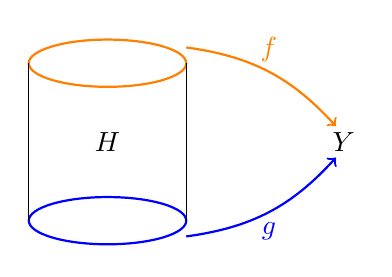
\begin{tikzpicture}
    \draw[blue, thick] (0, 0) ellipse(1 and 0.3);
    \draw[orange, thick] (0, 2) ellipse(1 and 0.3);

    \draw (-1, 0)--(-1, 2);
    \draw (1, 0)--(1, 2);

    \node at (3, 1) {$Y$};

    \path[->] (1, -0.2) edge [bend right=20, thick, blue] node [midway, below] {$g$} (2.9, 0.8);
    \path[->] (1, 2.2) edge [bend left=20, orange, thick] node [midway, above] {$f$} (2.9, 1.2);

    \node at (0, 1) {$H$};
  \end{tikzpicture}\end{center}

  Możemy do tego przyłożyć wiedzę o kompleksach, jeśli pod $X$ kryją się sympleksy. Wtedy mamy
  \begin{center}\begin{tikzpicture}[scale=1.5]
    \draw (0, 0) ellipse(1 and 0.3);
    \draw (0, 2) ellipse(1 and 0.3);

    \draw (-1, 0)--(-1, 2);
    \draw (1, 0)--(1, 2);

   % \draw[dashed] (-0.6, -0.1)--(-0.2, -0.15)--(-0.4, 0.1)--cycle;
   % \draw[dashed] (-0.4, 0.1)--(0, 0.15)--(-0.2, -0.15)--cycle;
   % \draw[dashed] (-0.2, -0.15)--(0.2, -0.15)--(0, 0.15)--cycle;
   % \draw[dashed] (0.2, -0.15)--(0.4 ,0.1)--(0, 0.15)--cycle;
   % \draw[dashed] (0.2, -0.15)--(0.4, 0.1)--(0.6, -0.1)--cycle;

    \draw[dashed] (-0.6, -0.1)--(-0.4, 0.1)--(-0.2, -0.15)--(0, 0.15)--(0.2, -0.15)--(0.4, 0.1)--(0.6, -0.1);
    \draw[dashed] (-0.4, 0.1)--(0, 0.15)--(0.4, 0.1);
    \draw (-0.6, -0.1)--(-0.2, -0.15)--(0.2, -0.15)--(0.6, -0.1);

    \draw (-0.6, 1.9)--(-0.2, 1.85)--(-0.4, 2.1)--cycle;
    \draw (-0.4, 2.1)--(0, 2.15)--(-0.2, 1.85)--cycle;
    \draw (-0.2, 1.85)--(0.2, 1.85)--(0, 2.15)--cycle;
    \draw (0.2, 1.85)--(0.4, 2.1)--(0, 2.15)--cycle;
    \draw(0.2, 1.85)--(0.4, 2.1)--(0.6, 1.9)--cycle;

    \draw(-0.6, -0.1)--(-0.6, 1.9);
    \draw(-0.2, -0.15)--(-0.2, 1.85);
    \draw(0.2, -0.15)--(0.2, 1.85);
    \draw(0.6, -0.1)--(0.6, 1.9);

    \draw[dashed] (-0.4, 0.1)--(-0.4, 2.1);
    \draw[dashed] (0, 0.1)--(0, 2.1);
    \draw[dashed] (0.4, 0.1)--(0.4, 2.1);

    \draw (2, 1.8)--(3, 2.2)--(1.8, 2.2)--cycle;
    \draw (2, -0.2)--(3, 0.2);
    \draw (2, -0.2)--(1.8, 0.2);
    \draw[dashed] (3, 0.2)--(1.8, 0.2);

    \draw (1.8, 0.2)--(1.8, 2.2);
    \draw (3, 0.2)--(3, 2.2);
    \draw (2, -0.2)--(2, 1.8);

    \node (HD) at (4, 1.5) {$H(\Delta)$};

    \path[->] (HD) edge [bend left=20] (2.4, 1);

    \node at (2.2, 2.1) {$\Delta$};
    \node at (2.5, -0.2) {$\partial$};

    \node at (4, 0.6) {$\substack{\partial H(\Delta)=f(\Delta)-g(\Delta)+\\+H(\partial\Delta)}$};
  \end{tikzpicture}\end{center}
\end{example}

\begin{fact}$ $

  \begin{enumerate}[label=(\alph*)]
    \item Relacja homotopijnej równoważności $\sim$ odwzorowań między ustalonymi kompleksami $A^*, B^*$ jest relacją równoważności
    \item Morfizmy $\sim 0$ tworzą "ideał", to znaczy 
      $$g, f\sim 0\implies f+g\sim 0$$
      $$(\forall\;k:B^*\to C^*,\; l:C^*\to A^*)\;f\sim 0\implies kf, fl\sim 0$$
    \item $f\sim g\implies H^i(f)=H^i(g)$
    \item Jeśli \begin{tikzcd}A^*\arrow[r, yshift=1mm, "f" above] & B^*\arrow[l, yshift=-1mm, "g" below]\end{tikzcd} są takie, że $fg\sim id_B$ oraz $gf\sim id_A$, to $f,g$ są qis oraz $H^i(f)=H^i(g)^{-1}$.
  \end{enumerate}
\end{fact}

\begin{proof}
  \begin{enumerate}[label=(\alph*)]
    \item Niech $f\overset{h}{\sim} g\overset{h'}{\sim} l$, wówczas $f\overset{h+h'}{\sim}l$. Wiemy więc, że 
      $$\begin{matrix}
        f-g = dh+hd\\ 
        g-l=dh'+h'd
      \end{matrix}$$
      dodając oba równania stronami, dostajemy
      $$f-l=(f-g)+(g-l)=(dh+hd)+(dh'+h'd)=(dh+dh')+(hd+h'd)=d(h+h')+(h+h')d.$$
    \item Jeśli $f, g\sim 0$ tak, że $f-0=dh+hd$ oraz $g-0=dh'+h'd$. Wtedy
      $$f+g=(f-0)+(g-0)=(dh+hd)+(dh'+h'd)=d(h+h')+(h+h')d.$$

      Pokażemy teraz, że dla $f\sim 0$ oraz dla dowolnego $k:B^*\to C^*$ mamy $kf\sim 0$. Rysując diagram
      \begin{center}
        \begin{tikzcd}[column sep=large, row sep=large, /tikz/column 1/.style={column sep=1mm}]
        A^*: & \bullet \arrow[d, "f" left] \arrow[r, dashed] & \bullet \tikzmark{A2} \arrow[d, "f" left] \arrow[r, dashed] \arrow[dl, "h" above] & \bullet \arrow[d, "f" left] \arrow[r, dashed] \arrow[dl, "h" above] & \bullet \arrow[d, "f" left] \\ 
        B^*: & \bullet \tikzmark{B1} \arrow[r, dashed] \arrow[d, "k" left] & \bullet \arrow[r, dashed, blue] \arrow[d, "k" left, red] & \bullet \arrow[r, dashed] \arrow[d, "k" left, blue] & \bullet \arrow[d, "k" left] \\ 
        C^*: & \bullet \tikzmark{C1} \arrow[r, dashed] & \bullet \arrow[r, dashed, red] & \bullet \arrow[r, dashed] & \bullet
        \end{tikzcd}
        
\begin{tikzpicture}[remember picture, overlay]
          \draw[orange, ->, rounded corners] ([xshift=-2mm, yshift=-2mm]pic cs:A2) to ([xshift=2mm, yshift=2mm]pic cs:B1) node [right] {$k\circ h$} to ([xshift=2mm, yshift=2mm]pic cs:C1);
        \end{tikzpicture}
      \end{center} 
      Wiemy, że $f^i=h^{i+1}d+dh^i$, a dalej
      $$k^if^i=k^i(h^{i+1}d+dh^i)=k^i(h^{i+1}d)+k^i(dh^i)=(k^ih^{i+1})d+({\color{red}k^{i}d})h^i=(k^ih^{i})d+{\color{blue}d(k^{i-1}}h^{i})$$

    \item Wystarczy sprawdzić, że $f\sim 0\implies H^i(f)=0$. Niech $[a]\in H^i(f)$ zadaje klasę kohomologii, czyli $a\mapsto 0$ przez różniczkę $A^i\to A^{i+1}$.
      \begin{center}
        \begin{tikzcd}[/tikz/row 1/.style={row sep=1mm}, /tikz/row 3/.style={row sep=1mm}]
          & a\arrow[d, phantom, sloped, "\in"] \arrow[r, mapsto] & 0 \\ 
          A^{i-1} \arrow[r] \arrow[d] & A^i \arrow[r] \arrow[d] \arrow[dl, "h^i" above, blue] & A^{i+1} \arrow[d] \arrow[dl, "h^{i+1}" above, blue] \\ 
          B^{i-1} \arrow[r] & B^i \arrow[r] & B^{i+1} \\ 
          ? \arrow[r, dashed] & f^i(a)\arrow[r, mapsto] \arrow[u, phantom, sloped, "\in"] & 0
        \end{tikzcd}
      \end{center}
      Wiemy, że 
      $$f^i(a)=h^{i+1}\underbrace{d(a)}_{=0}+dh^i(a)=dh^i(a)$$
      czyli $h^i(a)$ jest w ramach $?$.
    \item Wynika z warunku c).
  \end{enumerate}
\end{proof}

\subsection{Jednoznaczność rezolwenty projektywnej}

\begin{fact}
  Niech $P^*\to X$ oraz $Q^*\to Y$ będą rezolwentami projektywnymi, a $f:X\to Y$ będzie morfizmem.
  \begin{enumerate}
    \item Istnieje morfizm rezolwent $R(f):P^*\to Q^*$ rozszerzający $f$ w sensie komutowania driagramu
      \begin{center}\begin{tikzcd}
        ... \arrow[r] & P^0\arrow[r, "\epsilon_x"]\arrow[d, "R(f)^0"] & X \arrow[d, "f"] \\ 
        ... \arrow[r] & Q^0 \arrow[r, "\epsilon_y"] & Y
      \end{tikzcd}\end{center}
      oraz diagramów "dalej na lewo".
    \item $R(f)$ jak wyżej jest jedyny z dokładnością do homotopii.
  \end{enumerate}
\end{fact}

\begin{conclusion}
  Gdy $Y=X$ i $f=id_X$, to mamy jedyne z dokładnością do homotopii przekształcenie między dwoma różnymi rezolwentami $X$.

  \begin{center}\begin{tikzcd}
    P^*\arrow[r]\arrow[d, "R" right, bend left=20] & X\arrow[d, "id"]\\ 
    Q^*\arrow[r]\arrow[u, bend left=20, "L" left] & X
  \end{tikzcd}\end{center}
\end{conclusion}

\begin{proof}
  \begin{enumerate}[label=(\alph*)]
    \item Konstruujemy ten morfizm 
      \begin{center}\begin{tikzcd}
        P_0\arrow[r, "\epsilon_X"]\arrow[d, dashed] \arrow[dr, rounded corners, to path={([yshift=-4mm]\tikztostart) -| ([xshift=-5mm]\tikztotarget)}, blue] & X\arrow[r]\arrow[d, "f" right] & 0 \\ 
        Q_0\arrow[r, "\epsilon_Y" below] & Y \arrow[r] & 0
      \end{tikzcd}\end{center}
      Strzałka $P_0\to Q_0$ istnieje, ponieważ $P_0$ jest modułem projektywny, i $Q_0\to Y$ jest surjekcją (bo rezolwenta jest acykliczna). Czyli mamy komutujący diagram
      \begin{center}\begin{tikzcd}
        P_0\arrow[d, dashed]\arrow[dr, blue] \\ 
        Q_0\arrow[r] & Y \arrow[r] & 0
      \end{tikzcd}\end{center}
  Mamy więc pierwszy krok konstrukcji. Zakładamy teraz, że dla wszystkich $P_i\to Q_i$ o $i\leq n$ udało nam się skonstruować $R(f)^i$. Chcemy teraz korzystając z poprzednich korków aby skonstruować strałkę $P_{n+1}\to Q_{n+1}$:
  \begin{center}\begin{tikzcd}
    ... \arrow[r] & P_{n+1}\arrow[r, "d_{n+1}^P" above]\arrow[d, dashed] & P_n\arrow[r, "d_n^P" above]\arrow[d, "R(f)^n" right] & P_{n-1}\arrow[r]\arrow[d, "R(f)^{n-1}"] & ... \\ 
    ...\arrow[r] & Q_{n+1}\arrow[r, "d_{n+1}^Q" below] & Q_n\arrow[r, "d_n^Q" below] & Q_{n-1} \arrow[r] & ... 
  \end{tikzcd}\end{center}

  Mamy 
  $$0=R(f)^{n-1}d_n^Pd_{n+1}^P=d_n^QR(f)^nd_{n+1}^P$$
  w takim razie istnieje jedyna strzałka $P_{n+1}\to \ker d_n^Q$ i tak naprawdę tą strzałką jest "obcięcie" $R(f)^nd_{n+1}^P$ do $\ker d_n^Q$
  \begin{center}\begin{tikzcd}
    & P_{n+1}\arrow[d, "\exists!"] \arrow[dr, "d_{n+1}^PR(f)^n" above right]\\ 
    Q_{n+1}\arrow[r, "\exists!", twoheadrightarrow] & \ker d_n^Q = \img d_{n+1}^Q\arrow[r] & Q_n\arrow[r] & 0 
  \end{tikzcd}\end{center}
  ale ponieważ $\ker d_n^Q=\img d_{n+1}^Q$, to strzałka $Q_{n+1}\to \img d_{n+1}$ jest surjekcją. W takim razie z projektywności $P_{n+1}$ wiemy, że istnieje co najmniej jedna strzałka $P_{n+1}\to Q_{n+1}$ dzięki której komutuje diagram 
  \begin{center}\begin{tikzcd}
    & P_{n+1}\arrow[d]\arrow[dl, "\exists" above left]\\ 
    Q_{n+1}\arrow[r] & \ker d_n^Q\arrow[r] & 0
  \end{tikzcd}\end{center}
  
  Tak naprawdę interesuje nas diagram
  \begin{center}\begin{tikzcd}
    & P_{n+1}\arrow[d, "\exists p"] \arrow[dr, "d_{n+1}^PR(f)^n" above right]\arrow[dl, dashed, "R(f)^{n+1}" above left]\\ 
    Q_{n+1}\arrow[r, "\exists! u" below, twoheadrightarrow] & \ker d_n^Q = \img d_{n+1}^Q\arrow[r, "k"] & Q_n
  \end{tikzcd}\end{center}
  i upewnienie się, że $k\circ u \circ R(f)^{n+1}=d_{n+1}^P\circ R(f)^n$. Zauważmy, że $kp=d_{n+1}^PR(f)^n$, a z drugiej strony $p=uR(f)^{n+1}$, czyli $d_{n+1}^PR(f)^n=kp=kuR(f)^{n+1}$ tak jak chcieliśmy.
  \item Teraz szukamy $h$ który jest "świadkiem" homotopijnej równoważności dwóch możliwych $R(f)^i$ i $R(f')^i$, które będziemy oznaczać $f_i$ oraz $f_i'$.
    \begin{center}\begin{tikzcd}
      & P_0\arrow[dl, "h_0" above left]\arrow[r, "\epsilon_X"]\arrow[d, xshift=-1mm, "f_0" left] \arrow[d, xshift=1mm, "f_0'" right]& X\arrow[d, "f"] \arrow[r] & 0\\ 
      Q_1 \arrow[r] & Q_0\arrow[r, "\epsilon_Y"] & Y\arrow[r] & 0
    \end{tikzcd}\end{center}

    Zdefiniujmy $dh^0=f_0-f_0'$. Wtedy
    $$\epsilon_Y(dh^0)=\epsilon_Y(f_0-f_0')=\epsilon_Yf_0-\epsilon_Yf_0'=f\epsilon_X-f\epsilon_X=0.$$
    czyli $h^0$ istnieje, bo $dh^0=f_0-f_0'$ zachowuje się jak jądro $\epsilon_Y$ i możemy do 
    \begin{center}\begin{tikzcd}
      & P_0\arrow[d, "f_0-f_0'"]\arrow[dl, dashed] \\ 
      Q_1\arrow[r] & Q_0\arrow[r, "\epsilon_Y"] & Y\arrow[r] & 0 
    \end{tikzcd}\end{center}
    przyłożyć tę samą logikę co przy konstruowaniu $R(f)$.

    Przechodząc bardziej na lewo mamy diagram
    \begin{center}\begin{tikzcd}[column sep=large, row sep=huge]
      & P_i\arrow[dl, "h^i" above left]\arrow[r]\arrow[d, "f_i" left, xshift=-1mm]\arrow[d, xshift=1mm, "f_i'" right]\arrow[d, bend left=30, xshift=2mm, "\alpha"] & P_{i-1}\arrow[dl, "h^{i-1}"]\\ 
      Q_{i+1}\arrow[r] & Q_i\arrow[r] & Q_{i-1}
    \end{tikzcd}\end{center}
    gdzie $\alpha=f_i-f_i'-h^{i-1}d$. Jeśli $d\alpha=0$, to istnieje $h^i$ takie, że $\alpha=d h^i$, bo nadal działamy na projektywnych rezolwentach.
    \begin{align*}
      d\alpha&=d(f_i-f_i'-h^{i-1}d)=\\ 
             &=df_i-df_i'-dh^{i-1}d=\\ 
             &=(f_{i-1}-f_{i-1}'-dh^{i-1})d=\\ 
             &=(h^{i-2}d+dh^{i-1}-dh^{i-1})d=h^{i-2}dd=0
    \end{align*}
    Zatem $\alpha=f_i-f_i'-h^{i-1}d=dh^i$ i mamy wtedy
    $$f_i-f_i'=dh^i+h^{i-1}d$$
    tak jak w definicji homotopijnej równoważności.
\end{enumerate}
\end{proof}

Analogiczny fakt jest prawdziwy dla rezolwent injektywnych. W takim razie, dowolny obiekt $A$ rozumiany jako kompleks $...\to 0\to A\to 0\to...$ jest izomorficzny ze swoją rezolwentą injektywną i projektwyną w kategorii pochodnej $D(\mathbf{A})$.

\begin{example}
\item Niech $\mathbf{A}$ i $\mathbf{B}$ będą kategoriami abelowymi, a $T:\mathbf{A}\to \mathbf{B}$ addytywnym funktorem między tymi kategoriami.

  Weźmy obiekt $A\in\ob\mathbf{A}$ i dwie jego projektywne rezolwenty \begin{tikzcd}P^*\arrow[r, yshift=-1mm, "f" below]&Q^*\arrow[l, yshift=1mm, "g" above]\end{tikzcd}. Ponieważ $gf:P^*\to P^*$ i $fg:Q^*\to Q^*$ są odwzorowaniami między rezolwentami $A$, to są one homotopijnie równoważne z identycznością.
  
  Oczywiście $T(P^*)$ i $T(Q^*)$ są kompleksami:
  $$T(d)T(d)=T(dd)=T(0)=0$$
  z odwzorowaniami \begin{tikzcd}T(P^*)\arrow[r, yshift=1mm, "f" above] & T(Q^*)\arrow[l, yshift=-1mm, "g" below]\end{tikzcd} które również są homotopijne z identycznością:
  $$id-T(f)T(g)=T(id)-T(fg)=T(id-fg)=T(dh+hd)=T(d)T(h)+T(h)T(d).$$
  
  \begin{conclusion}
    $T(f)$ i $T(g)$ są wzajemnie odwrotnymi qis.
  \end{conclusion}
\end{example}


\newpage

\section{27.11.23 : Kategoria lokalna}

\begin{definition}[klasa lokalizująca]
  Klasa $S\subseteq Mor(\mathbf{B})$ jest nazywana \buff{lokalizującą}, jeśli spełnia następujące warunki:
  \begin{enumerate}
    \item identyczność dla dowolnego obiektu należy do $S$ i dla dowolnych $s,t\in S$ które można składać $s\circ t\in S$
    \item poniższe diagramy dopełniają się
      \begin{center}\begin{tikzcd}
        \bullet \arrow[r, dashed, green, "\in S"] \arrow[d, dashed] & \bullet\arrow[d] & & \bullet\arrow[r, green, "\in S"] \arrow[d] & \bullet\arrow[d, dashed]\\ 
        \bullet \arrow[r, green, "\in S" below] & \bullet & & \bullet\arrow[r, green, dashed, "\in S" below] & \bullet
      \end{tikzcd}\end{center}
      to znaczy, mając strzałki nieprzerywane znajdziemy strzałki przerywane tak, że odpowiednia strzałka jest z $S$ i powstałe diagramy komutują.
    \item dla wszystkich \begin{tikzcd}X\arrow[r, yshift=1mm, "f"]\arrow[r, yshift=-1mm, "g" below] & Y\end{tikzcd} $(\exists\;s\in S)\;(sf=sg)\iff ((\exists\;t\in S)\;ft=gt)$.
  \end{enumerate}
\end{definition}

\begin{definition}[domki]
  Niech $S$ będzie klasą lokalizującą w kategorii $\mathbf{B}$. Definiujemy nową kategorię $\color{green}\mathbf{B}[S^{-1}]$:
  \begin{itemize}
    \item $\ob \mathbf{B}[S^{-1}]=\ob \mathbf{B}$
    \item morfizmy $A\to A'$ to klasy równoważności "domków", czyli diagramów
      \begin{center}\begin{tikzcd}
        & B\arrow[dl, "s\in S", orange] \arrow[dr, "f"]\\ 
        A & & A' 
      \end{tikzcd}\end{center}
      które można rozumieć jako "ułamek" $fs^{-1}$.

      Mówimy, że dwa domki $B$ i $B'$ przedstawiające morfizm $A\to A'$ w $\mathbf{B}[S^{-1}]$ są równoważne, jeśli istnieje $C$ wraz z morfizmami (w $\mathbf{B}$) $C\to B$ i $C\to B'$ takimi, że poniższy domek komutuje
      \begin{center}\begin{tikzcd}
        & & C\arrow[dl, "r"]\arrow[dr] \arrow[ddll, orange, "sr\in S" above left, bend right=30]\\ 
        & B\arrow[dl, "s\in S" above left, orange]\arrow[drrr] & & B'\arrow[dr]\arrow[dlll, orange, "s'\in S" above left]\\ 
        A & & & & A'
      \end{tikzcd}\end{center}
  \end{itemize}
\end{definition}

Jeśli mamy domki $A\leftarrow B\to A'$ i $A' \leftarrow B'\to A''$, to ich złożeniem jest nowy domek, którego istnienie wynika z 2 warunku klasy lokalizujące:
\begin{center}\begin{tikzcd}
        & & C\arrow[dl, "s''\in S" above left, orange]\arrow[dr] \\ 
        & B\arrow[dl, "s\in S" above left, orange]\arrow[dr] & & B'\arrow[dr]\arrow[dl, orange, "s'\in S" above left]\\ 
        A & & A' & & A''
\end{tikzcd}\end{center}

\begin{theorem}[kategoria domków jest ciekawa]$ $

  \begin{enumerate}
    \item $\mathbf{B}[S^{-1}]$ jest dobrze określona:
      \begin{enumerate}
        \item relacja na domkach jest relacją równoważności 
        \item składanie domków nie zależy od wyboru reprezentantów
        \item składanie domków jest łączne
      \end{enumerate}
    \item Funktor $\mathbf{B}\to \mathbf{B}[S^{-1}]$ ma własność uniwersalną, tzn. jeśli mamy funktor $\mathbf{B}\to \mathbf{D}$ taki, że elementy klasy lokalizującej $S$ są przez niego posyłane na izomorfizmy w $\mathbf{D}$, to wówczas taki funktor faktoryzuje się przez $\mathbf{B}[S^{-1}]$:
      \begin{center}\begin{tikzcd}[column sep=large, row sep=small]
        \mathbf{B}\arrow[r]\arrow[ddr] & \mathbf{B}[S^{-1}]\arrow[dd, dashed]\\ 
        S\arrow[u, sloped, phantom, "\subseteq"]\arrow[ddr]\\
                                                                                               & \mathbf{D}\\ 
                                                                                               & \text{izo.}\arrow[u, sloped, phantom, "\subseteq"]
      \end{tikzcd}\end{center}
  \end{enumerate}
\end{theorem}

\begin{proof}
  \begin{enumerate}
    \item 
      \begin{enumerate}
        \item Jedyną ciekawą częścią tutaj jest sprawdzenie przechodności relacji równoważności domków. To znaczy, mając dane domki $A\leftarrow B\to A'\sim A\leftarrow B'\to A'$ oraz $A\leftarrow B'\to A'\sim A\leftarrow B''\to A'$ chcemy znaleźć dowód na równoważność domków $B$ i $B''$:
          \begin{center}\begin{tikzcd}
            & & D\arrow[dr, dashed]\arrow[dl, dashed]\\
            & C \arrow[dl]\arrow[dr] & & C'\arrow[dl]\arrow[dr]\\
            B\arrow[d, orange]\arrow[drrrr] & & B'\arrow[dll, orange]\arrow[drr] & & B''\arrow[d]\arrow[dllll, orange]\\
            A & & & & A'
          \end{tikzcd}\end{center}
          Obiekt $D$ wraz ze strzałkami $D\to C$ oraz $D\to C''$ dostajemy z warunku 2. klasy lokalizującej:
          \begin{center}\begin{tikzcd}[column sep=tiny, row sep=tiny]
              &   & D\arrow[ddll, orange]\arrow[ddrr] \\
              & {\color{white}d} \\ 
            C\arrow[dr]\arrow[ddrr, orange, bend right=30] &   &   &    & C'\arrow[dl]\arrow[ddll, orange, bend left=30] \\ 
                                                           & B \arrow[dr, orange] &   & B'\arrow[dl, orange]     \\ 
              &   & A
          \end{tikzcd}\end{center}

      Z tak uzyskanym $D$ chcemy sprawdzić przemienność diagramu na fragmencie 
      \begin{center}\begin{tikzcd}
        & D\arrow[dl, orange]\arrow[dr] \\ 
        B\arrow[d, orange]\arrow[drr] & & B''\arrow[d]\arrow[dll, orange]\\ 
        A & & A' 
      \end{tikzcd}\end{center}
      narysujmy to w mniej konserwatywny sposób:
      \begin{center}\begin{tikzcd}
        & D'\arrow[d, "t", orange]\\ 
        & D\arrow[dr]\arrow[dl, orange]\arrow[dd, bend right=40, "f" right]\arrow[dd, bend left=40, "g" left]\\ 
        C\arrow[dr] & & C'\arrow[dl]\\ 
                    & B\arrow[d, "s", orange]\\ 
                    & A
      \end{tikzcd}\end{center}
      Na diagramie wyżej potencjalnym problemem jest uzyskanie $f=g$. Ale ponieważ mamy $sf=sg$ i $s\in S$, to z warunku klasy lokalizującej możemy znaleźć $t$ takie, że $ft=gt$. Wtedy wystarczy podmienić $D$ na $D'$ i wszystko nad $B$ się zgadza.
    \item Niezależność wyniku złożenia domków od wyboru reprezentantów. Pokażemy tylko połowę tego dowodu, tę odpowiedzialną za niezależność wyboru lewego domku.

      Mamy więc równoważne domki
      \begin{center}\begin{tikzcd}
        & C''\arrow[dl]\arrow[dr]\\ 
        B\arrow[d, orange]\arrow[drr] & & B'\arrow[d]\arrow[dll, orange]\\ 
        A & & A' 
      \end{tikzcd}\end{center}
      oraz kolejny domek \begin{tikzcd}A' & B''\arrow[l, orange]\arrow[r] & A''\end{tikzcd}. Składanie domków daje diagram
      \begin{center}\begin{tikzcd}
        C''\arrow[d]\arrow[dr] & C\arrow[dr]\arrow[dl, orange] & C'\arrow[d]\arrow[dl, orange] \\ 
        B \arrow[d, orange]\arrow[drr]& B'\arrow[d]\arrow[dl, orange] & B''\arrow[dl, orange]\arrow[d] \\ 
        A & A' & A''
      \end{tikzcd}\end{center}
      naszym celem będzie pokazanie, że domki $C$ i $C'$ przychodzące ze składania domków $B$ są równoważne.

      Patrząc na kwadrat \begin{tikzcd} C''\arrow[r] & B & \arrow[l, orange] C\end{tikzcd} dostajemy \begin{tikzcd}C'' & D\arrow[r, orange] \arrow[r] & C\end{tikzcd} natomiast z kwadratu \begin{tikzcd} C'' \arrow[r] & B' & C'\arrow[l, orange]\end{tikzcd} dostajemy \begin{tikzcd}C'' & D'\arrow[l, orange]\arrow[r] & C'\end{tikzcd}. Mając już $D$ i $D'$ możemy wytworzyć $E$ z kwadratu \begin{tikzcd}D\arrow[r, orange] & C'' & D'\arrow[l, orange]\end{tikzcd}. Dostajemy diagram
      \begin{center}\begin{tikzcd}
        & E\arrow[dl, orange]\arrow[dr]\\
        D\arrow[d, orange]\arrow[dr] & & D'\arrow[dl, orange]\arrow[d]\\
        C''\arrow[d]\arrow[dr]\arrow[dd, bend right=20, orange] & C\arrow[dr]\arrow[dl, orange] & C'\arrow[d]\arrow[dl, orange] \\ 
        B \arrow[d, orange]\arrow[drr]& B'\arrow[d]\arrow[dl, orange] & B''\arrow[dl, orange]\arrow[d] \\ 
        A & A' & A''
      \end{tikzcd}\end{center}
      Do diagramu którego potrzebujemy trafią wierzchołki $E, C, C', A, A''$ więc chcemy, żeby taki diagram komutował i zawsze spełniał $E\to A\in S$. Zaczniemy od pokazania, że ścieżka $E\to D\to C\to B\to A$ jest w klasie $S$:
      \begin{center}\begin{tikzcd}
        E\arrow[r, orange] & D\arrow[r]\arrow[dr, orange] & C\arrow[r, orange] & B\arrow[r, orange] & A\\ 
                           & & C''\arrow[ur]\arrow[urr, orange, bend left=10]
      \end{tikzcd}\end{center}
      obie ścieżki są sobie równe, więc jedyna podejrzana ścieżka $E\to A$ leży w $S$.

      Sprawdzimy teraz komutowanie ostatecznego diagramu
      \begin{center}\begin{tikzcd}
        & E\arrow[dl, orange]\arrow[dr]\\ 
        C\arrow[d, orange]\arrow[drr] & & C'\arrow[d]\arrow[dll, orange]\\ 
        A & & A'' 
      \end{tikzcd}\end{center}
      poprzez przebudowanie ścieżki $E\to D\to C\to B\to A$ tak, aby dostać $E\to D'\to C'\to B'\to A$ (i analogicznie ze ścieżkami $E\to A''$, ale to pominiemy)
      \begin{center}\begin{tikzcd}
        E\arrow[r, orange]\arrow[dr] & D\arrow[r] & C \arrow[r, orange] & B \arrow[r, orange] & A \\ 
                                     & D' \arrow[ur, orange] \arrow[r] & C'\arrow[r, orange] & B'\arrow[ur, orange]
      \end{tikzcd}\end{center}
    \end{enumerate}
  \item Funktor $\mathbf{B}\to \mathbf{B}[S^{-1}]$ jest identycznością na obiektach, natomiast morfizm $f:X\to Y$ zamieniamy na domek
  \begin{center}\begin{tikzcd}
    & X\arrow[dl, orange, "id_X\in S" above left]\arrow[dr, "f"]\\ 
    X & & Y
  \end{tikzcd}\end{center}
  Zauważmy tutaj, że elementy $s\in S$ przechodzą przez ten funktor na izomorfizmy, gdyż mamy następujące domki
  \begin{center}\begin{tikzcd}
    & X\arrow[dl, "id\in S" above left, orange] \arrow[dr, "s" above right] & & & X\arrow[dl, "s\in S" above left, orange]\arrow[dr, "id" above right] \\ 
    X & & Y & Y & & X
  \end{tikzcd}\end{center}
  które składają się do 
  \begin{center}\begin{tikzcd}
    & X\arrow[dl, "id" above left, orange]\arrow[dr, "id" above right] & & & & X\arrow[dr, "id" above right]\arrow[dl, orange, "id" above left]\\ 
    X\arrow[d, "id" left, orange]\arrow[dr, "s" above right] & & X\arrow[dl, "s" above left, orange]\arrow[d, "id"  right] & & X\arrow[d, orange, "s" left]\arrow[dr, "id" above right] & & X\arrow[dl, "id" above left, orange]\arrow[d, "s" right] \\ 
    X & Y & X & & Y & X & Y
  \end{tikzcd}\end{center}
  gdzie domek po prawej jest równoważny identyczności na $Y$.

  Tak zdefiniowany funktor $\mathbf{B}\to \mathbf{B}[S^{-1}]$ spełnia własność uniwersalną, tzn istnieje funktor $\overline{T}$ taki, że komutuje diagram
  \begin{center}\begin{tikzcd}
    \mathbf{B}\arrow[r]\arrow[dr, "T" below left] & \mathbf{B}[S^{-1}]\arrow[d, dashed, "\overline{T}" right]\\ 
                                  & \mathbf{D}
  \end{tikzcd}\end{center}
  Funktor $\overline{T}$ definiujemy na morfizmach, czyli domkach jako
  $$
  \overline{T}(A \xleftarrow{s}B\xrightarrow{f} A') = 
  T(f)\circ T(s)^{-1}.
  $$
  Tak zdefiniowany funktor nie zależy od wyboru reprezentanta domku, tzn. wybierzmy
  \begin{center}\begin{tikzcd}
    & C\arrow[dl, "t" above left, orange]\arrow[dr, "g"]\\ 
    B\arrow[d, "s" left, orange]\arrow[drr, "f" near start] & & B'\arrow[dll, orange, "s'" near start]\arrow[d, "f'" right]\\ 
    A & & A'
  \end{tikzcd}\end{center}
  \begin{align*}
    \overline{T}(\uparrow)&=T(f)T(s)^{-1}=T(ft)T(st)^{-1}=\\ 
                          &=T(f)T(t)T(st)^{-1}=T(f')T(g)T(st)^{-1}=\\ 
                          &=T(f')T(g)T(s'g)^{-1}=T(f')T(g)T(g)^{-1}T(s')^{-1}\\ 
                          &=T(f')T(s')^{-1}
  \end{align*}
  \end{enumerate}
\end{proof}

\subsection{Quasi-isomorfizmy tworzą klasę lokalizującą}

\begin{theorem}$ $

  \begin{enumerate}
    \item Qis tworzą klasę lokalizującą w kategorii homotopijnej $K(\mathbf{A})$ ($\ob K(\mathbf{A})=\ob Kom(\mathbf{A})$, a morfizmy to klasy homotopii morfizmów w $Kom(\mathbf{A})$.)
    \item $K(\mathbf{A})[qis^{-1}]=D(\mathbf{A})$.
  \end{enumerate}
\end{theorem}




\newpage

\section{04.12.23 : Kategoria pochodna jako kategoria zlokalizowana}

\subsection{Quasi-izomorfizmy tworzą klasę lokalizującą}

\begin{theorem}
  qis tworzą w $K(\mathbf{A})$ klasę lokalizującą.
\end{theorem}

\begin{proof}
  \begin{enumerate}
    \item Składanie morfizmów jest oczywiste
    \item Uzupełniają się diagramy
      \begin{center}\begin{tikzcd}
        D^*\arrow[r, "qis" above]\arrow[d] & C^*\arrow[d, "g"] \\ 
        A^*\arrow[r, "s" above, "qis" below] & B^*
      \end{tikzcd}\end{center}

      \begin{center}\begin{tikzcd}
        {\color{red}(C(\tau))[-1]}\arrow[d, dashed]\arrow[r, dashed] & B^*\arrow[r, "\tau"], \arrow[d, phantom, sloped, "="] & C(s)\arrow[r]\arrow[d, phantom, sloped, "="] & C(\tau)\arrow[d] \\ 
        A^*\arrow[r, "s"] & B^*\arrow[r, "\tau"] &C(s) \arrow[r] & A^*[1]
      \end{tikzcd}\end{center}
      jest z poprzedniego wykładu, teraz chcemy do niego dopisać linijkę na górze

      \begin{center}\begin{tikzcd}
        C(\tau g)[-1]\arrow[r, green]\arrow[d] & C^*\arrow[d, "g"] \arrow[r, "\tau g"] & C(s) \arrow[d, phantom, sloped, "="] \arrow[r] & C(\tau g)\arrow[d, green] \\
        {\color{red}(C(\tau))[-1]}\arrow[d, dashed]\arrow[r, dashed] & B^*\arrow[r, "\tau"], \arrow[d, phantom, sloped, "="] & C(s)\arrow[r]\arrow[d, phantom, sloped, "="] & C(\tau)\arrow[d] \\ 
        A^*\arrow[r, "s"] & B^*\arrow[r, "\tau"] &C(s) \arrow[r] & A^*[1]
      \end{tikzcd}\end{center}

        Pojawia nam się szukany fragment (dwie pierwsze kolumny). Ponieważ $s$ jest qis, to $H^*(A^*)\to H^*(B^*)$ są izomorfizmami, a więc z ciągu dokładnego kohomologii wiemy, że $H^*(C(s))=0$. Ponieważ $C(s)$ jest takie samo na dole jak na górze, to wiemy, że $H^*(C(\tau g))[-1]\to H^*(C^*)$ jest izomorfizmem, co z definicji daje, że $C(\tau g)[-1]\to C^*$ jest qis.

      \item $sf=0$ w $K(\mathbf{A})$ (czyli $sf\overset{h}{\sim} 0$ w $Kom(\mathbf{A})$), to istnieje $t$ qis taki, że $ft=0$ w $K(\mathbf{A})$.

        Znowu rysujemy diagram 
        \begin{center}\begin{tikzcd} 
          &C(s)[-1]\arrow[d, phantom, sloped, "="] \arrow[r] & B^*\arrow[r, "s"] & \overline{B^*} \arrow[r] & C(s)\\ 
          C(g)&C(s)[-1]\arrow[l]& A^*\arrow[u, "f"]\arrow[l, "g"] & C(g)[-1]\arrow[l, "t"] \\ 
          &(f(a^i), -h(a^i))\arrow[u, sloped, phantom, "\in"] & a^i\arrow[l, mapsto]\arrow[phantom, sloped, u, "\in"]
        \end{tikzcd}\end{center}

        Jako ćwiczenie pozostaje sprawdzenie, że $gd=dg$.

        Ponieważ $s$ jest qis, to $C(s), C(s)[-1]$ są kompleksami acyklicznymi. Z tego wynika, że $t$ jest qis. 

        {\large\color{red}TUTAJ JESZCZE OBRAZKI ZE ZDJECIA}
  \end{enumerate}
\end{proof}

\subsection{Homotopie są tym samym w kat. pochodnej}

\begin{lemma}
  Niech $f,g:A^*\to B^*$ będą odwzorowaniami łańcuchowymi i $f\sim g$. Wtedy $Q(f)=Q(g)$, czyli indukują to samo w kategorii pochodnej $D(\mathbf{A})$.
\end{lemma}

Szybkie wytłumaczenie:
\begin{center}\begin{tikzcd}
   & f\sim g\\
  & Kom(\mathbf{A}) \arrow[dr, "Q"]\arrow[dl] \\ 
  K(\mathbf{A})[qis^{-1}] & & D(\mathbf{A})\arrow[ll]\\ 
  K(f)=K(g) & & Q(f), Q(g)\arrow[ll, mapsto]
\end{tikzcd}\end{center}

\begin{definition}
  Jeśli $A^*$ jest kompleksem, to kompleks $A^*\times I$ jest definiowany jako 
  $$(A^i\times I)^i=A^i\oplus A^{i+1}\oplus A^i$$
  z różniczką
  $$d(a^i, a^{i+1}, a'^i)=(da^i-a^{i+1}, -da^{i+1}, da'^i+a^{i+1})$$
\end{definition}

Tak zdefiniowany kompleks $A^*\times I$ jest związany z kompleksem $A^*$, m.in. istnieją włożenia i rzuty:
\begin{center}\begin{tikzcd}
  & (a^i, 0, 0) \\
  a^i\arrow[ur, "i_0"] \arrow[dr, "i_1"]& & & (a^i, a^{i+1}, a'^i)\arrow[r, mapsto, "p"] & (a^i+a'^i)\\ 
  & (0, 0, a^i)
\end{tikzcd}\end{center}

\begin{lemma}[a dokładniej to podlemat]
  $i_0p\sim id_{A^*\times I}\sim i_1p$, zatem $i_0$ oraz $i_1$ są qis odwrotnymi do qis $p$. W takim razie w kategorii pochodnej $D(\mathbf{A})$ mamy 
  $$Q(p)^{-1}=Q(i_0)=Q(i_1)$$
\end{lemma}

\begin{proof}
  Dowód dla $i_0$:
  \begin{align*}
    h(a^i, a^{i+1}, a'^i)&=(0, a'^i, 0)\\ 
    dh(a^i, a^{i+1}, a'^i) &= (-a'^i, -da'^i, a'^i)\\ 
    hd(a^i, a^{i+1}, a'^i) &= (0, da'^i+ a^{i+1}, 0)\\ 
    dh+hd (a^i, a^{i+1}, a'^i)&=()
  \end{align*}


\begin{center}\begin{tikzcd}
  & (a^i+a'^i, 0, 0) \arrow[dr]\\
  (a^i, a^{i+1}, a'^i)\arrow[ur, "i_0p"] \arrow[dr, "id"] & & (-a'^i, a^{i+1}, a'^i) \\ 
  & (a^i, a^{i+1}, a'^i)\arrow[ur]
\end{tikzcd}\end{center}
Czyli $dh+hd=id-i_0p$.

\end{proof}

\begin{proof}
  Dowód lematu wyżej.

  Niech $f\overline{h}{\sim} g$. Przerobimy to na $H:A^*\times I\to B^*$ tak, że 
  $$Hi_0=f, Hi_1=g.$$
  Wzorem zapisuje się to 
  $$H(a^i, a^{i+1}, a'^i)=f(a^i)+h(a^{i+1})+g(a'^i).$$
  Chcemy sprawdzić, że jest to łańcuchowe. 
  \begin{center}\begin{tikzcd}
    (a^i, a^{i+1}, a'^i) \arrow[r, "H"]\arrow[d, "d"] & {\color{red}f(a^i)} +h(a^{i+1})+{\color{red}g(a'^i)}\\ 
    ({\color{green}da^i-a^{i+1}}, -da^{i+1}, da'^i+a^{i+1}) \arrow[r, "H"] & \substack{
      {\color{green}(}{\color{red}df(a^i)}-f(a^{i+1}){\color{green})}+ \\ -hda^{i+1}+ \\ +{\color{red}dg(a^i)}+g(a^{i+1})
    }
  \end{tikzcd}\end{center}
  $$Q(f)=Q(Hi_0)=Q(H)Q(i_0)=Q(H)Q(i_1)=Q(Hi_1)=Q(g)$$
\end{proof}

\subsection{Równoważność domków i qis}

\begin{fact}
  $$K(\mathbf{A})[qis^{-1}]=D(\mathbf{A})$$
\end{fact}

\begin{proof}
  Zaczynamy od diagramu, na którym się to wszystko opiera 
  \begin{center}\begin{tikzcd}
    & Kom(\mathbf{A}) \arrow[dl] \arrow[dr, "Q"] \\ 
    K(\mathbf{A})[qis^{-1}] & & D(\mathbf{A})\arrow[ll]
  \end{tikzcd}\end{center}
  na obiektach to wszystko jest identycznością. Na morfizmach strzałka $D(\mathbf{A})\to K(\mathbf{A})[qis^{-1}]$ jest surjektywna: $Q(f)Q(s)^{-1}$ przechodzi na element
  \begin{center}\begin{tikzcd}
    & B\arrow[dl, "s" above left]\arrow[dr, "f"] &    &   & B\arrow[dl, "s" above left] \arrow[dr, "id"] &   & B\arrow[dl, "id" above left]\arrow[dr, "f"] \\ 
    A &                               & A' & A &                                   & B & & A
  \end{tikzcd}\end{center} 
  Chcemy teraz pokazać, że $D(\mathbf{A})\to K(\mathbf{A}[qis^{-1}]$ jest też $1-1$. Z każdego morfizmu w $D(\mathbf{A})$ pojawi się domek w $K(\mathbf{A})[qis^{-1}]$. Każda strzałka w $D(\mathbf{A})$ to jeden domek. Ale ponieważ umiemy domki składać, to 
  \begin{center}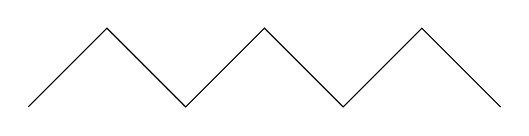
\begin{tikzpicture}
    \draw(0, 0)--(1, 1)--(2, 0)--(3, 1)--(4, 0)--(5, 1)--(6, 0);
  \end{tikzpicture}\end{center}
  {\large\color{red}TUTAJ OBRAZKI ZE ZDJĘĆ}

  Każdy morfizm w $D(\mathbf{A})$ jest dany domkiem postaci 
  \begin{center}\begin{tikzcd}
    & .\arrow[dl, "S"]\arrow[dr, "F"]\\ 
    . & & . 
  \end{tikzcd}\end{center}
  gdzie $S$ jest qis. To znaczy, że każdy domek jest postaci $Q(F)Q(S)^{-1}$. Załóżmy więc, że mamy diagram
  \begin{center}\begin{tikzcd}
    B\arrow[r, "F"]\arrow[d, "S"] & A'\\ 
    A & B'\arrow[l, "S'"] \arrow[u, "F'"]
  \end{tikzcd}\end{center}
  gdzie góra i dół przechodzi na to samo, mianowicie
  \begin{center}\begin{tikzcd}
      &   & C\arrow[dl, "T"] \arrow[dr, "G"] \\ 
      & B \arrow[dl, "S"]\arrow[drrr, "F"] & & B' \arrow[dr, "F'"]\arrow[dlll, "S'"] \\ 
    A &   & &   & A'
  \end{tikzcd}\end{center}
  \begin{align*}
    Q(F)Q(S)^{-1}&=Q(F)Q(T)Q(T)^{-1}Q(S)^{-1}=Q(FT)Q(ST)^{-1}=Q(F'G)Q(ST)^{-1}= \\ 
                 &=Q(F'G)Q(S'G)^{-1})=Q(F')Q(G)Q(G)^{-1}Q(S')^{-1}=Q(F')Q(S')^{-1}
  \end{align*}
\end{proof}

\begin{example}
\item $A=Vect_K$, wtedy 
  $$D(\mathbf{A})=\prod_{n=-\infty}^\infty \mathbf{A}[n]=Kom_0(\mathbf{A})$$
  to po prawej to kompleksy łańcuchowe z zerowymi różniczkami.

  \begin{center}\begin{tikzcd}
    Kom(\mathbf{A}) \arrow[rr, "H^*", yshift=1mm] \arrow[dr] & & Kom_0(\mathbf{A})\arrow[ll, yshift=-1mm, hookrightarrow]\arrow[dl, "l" above left, yshift=1mm] \\ 
       & D(\mathbf{A})\arrow[ur, "k" below right, yshift=-1mm]
  \end{tikzcd}\end{center}
  Tutaj $lk\sim id_{D(\mathbf{A})}$ jest homotopijne.
\end{example}

\subsection{Pomiędzy nami, obiektami, a wszystkimi kompleksami}

\begin{definition}
  $A^*\in Kom(\mathbf{A})$ jest $H^0$-kompleksem, jeśli $H^i(A^*)=0$ dla $i\neq 0$.
\end{definition}

\begin{fact}\label{fakt 10.5}
  Jeśli popatrzymy na funktor $\mathbf{A}\to D(\mathbf{A})$
  $$A\mapsto (...\to 0\to A\to 0\to ...)$$
  to taki funktor jest równoważnością między $A$ i pełną podkategorią $D(\mathbf{A})$ rozpiętą na $H^0$-kompleksach.
\end{fact}

$(...\to0\to A\to0\to...)$ oznacza się $A[0]$ lub nawet $A$.

\begin{proof}
  Nazwijmy badany funktor $F$. Pokażemy, że jest on wiermy, pełny i w zasadzie surjektywny.

  $$Hom_{\mathbf{A}}(X, Y)=Hom_{K(\mathbf{A})}(X, Y)$$
  są praktycznie takie same, bo jeśli $\phi: X\to Y$, to po prawej stronie mamy
  \begin{center}\begin{tikzcd}
    ...\arrow[r] & 0\arrow[r] \arrow[d] & X\arrow[r]\arrow[d, "\phi"] \arrow[dl, blue] & 0\arrow[r] \arrow[d] \arrow[dl, blue] & ... \\ 
    ...\arrow[r] & 0\arrow[r] & Y \arrow[r] & 0\arrow[r] & ...
  \end{tikzcd}\end{center}
  i wszystkie możliwe homotopie są między $0$ lub z/do $0$, więc one same też są zerowe.

  Dalej niech \begin{tikzcd}Hom_{K(\mathbf{A})}(X, Y)\arrow[r, yshift=1mm, "a"] & Hom_{D(\mathbf{A})}(X, Y)\arrow[l, "b=H^0", yshift=-1mm]\end{tikzcd}. Od razu można zauważyć, że $b\circ a=id$, więc pytamy tylko o $a\circ b$. Mamy 
  {\large\color{red}KOLEJNY RYSUNEK}
\end{proof}

\newpage

\section{11.12.23 : Rozszerzenia (extensions) Ext}
 
\begin{definition}[$Ext^i_{\mathbf{A}}(X, Y)$]
  Niech $\mathbf{A}$ będzie kategorią abelową. Rozważamy kategorie $Kom(\mathbf{A}), K(\mathbf{A}), D(\mathbf{A})$, które wszystkie mają te same obiekty.

  Niech $X\in\mathbf{A}$ będzie obiektem. Wtedy $\color{blue}X[-i]$ jest kompleksem, w który na $i$-tym miejscu stoi $X$:
  \begin{center}\begin{tikzcd}[row sep=tiny]
    ...\arrow[r] & 0\arrow[r] & X\arrow[r] & 0\arrow[r] & ... \\ 
                 & & i
  \end{tikzcd}\end{center}

  Dla $X,Y\in\ob\mathbf{A}$ definiujemy
  $$\color{blue}Ext_{\mathbf{A}}^i(X, Y)=Hom_{D(\mathbf{A})}(X[0], Y[i])$$
\end{definition}

Powyższe kategorie niekoniecznie są abelowe, ale na pewno są addytywne, więc na $Hom$ jak wyżej mamy zdefiniowaną operację dodawania.

Zauważmy, że
$$Hom_{D(\mathbf{A})}(X[0], Y[i])\cong Hom_{D(\mathbf{A})}(X[l], Y[i+l]).$$
możemy więc na $Ext$ zdefiniować mnożenie:
\begin{definition}[mnożenie $Ext$]
  $$Ext_{\mathbf{A}}^i(X, Y)\times Ext_{\mathbf{A}}^j(Y, Z)\xrightarrow{} Ext_{\mathbf{A}}^{i+j}(X, A)$$
  takie, że
  $$(X[0]\to Y[i])(Y[i]\to Z[j+i])\mapsto(X[0], Z[i+j])$$
\end{definition}

\subsection{Konstrukcja Yonedy}

Niech będzie dany ciąg dokładny
\begin{center}\begin{tikzcd}
  ...\arrow[r] & 0\arrow[r] & Y^{-i}\arrow[r] & K^{-i+1}\arrow[r] & ...\arrow[r] & K^0\arrow[r] & X\arrow[r] & 0\arrow[r] & ...
\end{tikzcd}\end{center}

Możemy wziąć fragment tego ciągu aż do $X$ i dopełnić go $0$. Dostajemy ciąg który nie jest już dokładny, więc dokładamy mu $X$ na dole, czyli tak naprawdę tworzymy odwzorowanie w kompleks $X[0]$ i drugie w kompleks $Y[i]$:
\begin{center}\begin{tikzcd}
  0\arrow[r] & Y\arrow[r]\arrow[d, "id"] & K^{-i+1}\arrow[r] & ... \arrow[r] & K^{0}\arrow[r]\arrow[d, "qis"] & 0\\ 
             & Y[i] & & & X[0]
\end{tikzcd}\end{center}
Tworzy się więc domek:
\begin{center}\begin{tikzcd}
  & K^*\arrow[dl, "qis" above left] \arrow[dr] \\ 
  X[0] & & Y[i] 
\end{tikzcd}\end{center}
Który nazywamy $Y(K^*)$ i jest on wtedy elementem $Ext_{\mathbf{A}}^i(X, Y)$.

\begin{example}
  \item $...\to Y\to K^0\to 0\to ... \in Ext^1(X, Y)$, wtedy domek 
    \begin{center}\begin{tikzcd}[column sep=tiny]
      & ...\to Y\to K^0\to 0\to ... \arrow[dl] \arrow[dr] \\ 
      X[0] & & Y[1] 
    \end{tikzcd}\end{center}
    można zamienić na ciąg dokładny
    \begin{center}\begin{tikzcd}
      0\arrow[r] & Y \arrow[r] & K^0\arrow[r] & X\arrow[r] & 0 
    \end{tikzcd}\end{center}
    $K^0$ jest rozszerzeniem (extension) obiektu $X$ przez obiekt $Y$
  \item W kategorii przestrzeni wektorowych $Vect_K$ wszystkie $Ext=0$.
  \item W kategorii grup abelowych $\mathbf{Ab}$ mamy 
    \begin{center}\begin{tikzcd}
      0\arrow[r] & \Z\arrow[r, "2\times"] & \Z \arrow[r] & \Z/2\Z\arrow[r] & 0 
    \end{tikzcd}\end{center}
    czyli nietrywialny element w $Ext^1_{\mathbf{Ab}}(\Z/2\Z, \Z)$.
\end{example}

\begin{theorem}[postaci $Ext$]$ $

  \begin{enumerate}[label=(\alph*)]
    \item Dla $i>0$ każdy element grupy $Ext_{\mathbf{A}}^i(X, Y)$ jest postaci $Y(K^*)$. To znaczy, że domki konstruowane wyżej są przydatne.
    \item $Ext^0(X, Y)=Hom_{D(\mathbf{A})}(X[0], Y[0])=Hom_{\mathbf{A}}(X, Y)$ (było tydzień temu \ref{fakt 10.5})
    \item Dla $i<0$ $Ext^i(X, Y)=0$.
  \end{enumerate}
\end{theorem}

\begin{proof}
  \begin{enumerate}[label=(\alph*)]
    \setcounter{enumi}{2}
    \item Zaczynamy od diagramu dla $A^*\in Hom_{D(\mathbf{A})}(X[0], Y[i])$
      \begin{center}\begin{tikzcd}
        & A^*\arrow[dl, "s" above left]\arrow[dr, "f" above right] \\ 
        X[0] & & Y[i] \\ 
             & B^*\arrow[ul, "s'" below left, orange]\arrow[ur, "0" below right, orange] \arrow[uu, "t", orange]
      \end{tikzcd}\end{center}
      pokażemy, że te pomarańczowe strzałki da się dorysować, by cały diagram komutował.

      Niech $B^*$ będzie kompleksem
      \begin{center}\begin{tikzcd}
        B^*=...\arrow[r] & A^{-i-2}\arrow[r] & \ker d^{-i-1}\arrow[r] & 0\arrow[r] & ... 
      \end{tikzcd}\end{center}
      czyli nad $Y$ ma zero, a nad $X$ ma bardzo podobny wygląd - na pewno homologie w $X$ się nie różnią od homologii w $X$ w kompleksie $A^*$:

      \begin{center}\begin{tikzcd}[column sep=small]
        A^*: ...\arrow[r]  & A^0\arrow[r] & ... \arrow[r] & A^{-i-2}\arrow[r] & A^{-i-1}\arrow[r] & A^{-i}\arrow[r] & A^{-i+1} \arrow[r] & ...\\ 
        X[0]: ...\arrow[r] & X\arrow[r]   & 0\arrow[r] & ... &    Y[i]:...\arrow[r] & Y     \arrow[r]   & 0     \arrow[r] & ...\\ 
        %Y[i]: ...\arrow[r] & 0\arrow[r]   & ...\arrow[r]  & 0\arrow[r]        & 0\arrow[r]        & Y\arrow[r]      & 0\arrow[r]         & ...\\ 
        B^*:  ...\arrow[r] & A^0\arrow[r] & ...\arrow[r]  & A^{-i-2}\arrow[r] & \ker d^{-i-1}\arrow[r] & 0\arrow[r] & 0\arrow[r]         & ...
      \end{tikzcd}\end{center}

      Nowy, zerowy, domek 
      \begin{center}\begin{tikzcd}
        & B^*\arrow[dr, "0" above right] \arrow[dl, "s'" above left] \\ 
        X[0] & & Y[i]
      \end{tikzcd}\end{center}
      dominuje stary domek z $A^*$, więc ten stary też musiał być zerowy. Stąd każdy element $Ext^i_{\mathbf{A}}(X, Y)$ jest zerowym domkiem.
    
    \setcounter{enumi}{0}
    \item Zaczynamy od kompleksu $K^*$ i cały manewr będzie polegał na usunięciu wszystkiego, co nie jest między $-i$ a $0$. Mamy dany diagram
      \begin{center}\begin{tikzcd}
        & K^*\arrow[dl]\arrow[dr] \\ 
        X[0] & & Y[i]
      \end{tikzcd}\end{center}
      a po wycinance
      \begin{center}\begin{tikzcd}[column sep=small]
        ...\arrow[r] & K^{-i-1}\arrow[r] & K^{-i}\arrow[r] & K^{-i+1}\arrow[r] & ... \arrow[r] & K^{-1}\arrow[r] & K^0\arrow[r] & K^1\arrow[r] & ...\\ 
        ...\arrow[r] & K^{-i-1}\arrow[r]\arrow[u, "qis"]\arrow[d, "qis" left] & K^{-i}\arrow[r]\arrow[u]\arrow[d] & K^{-i+1}\arrow[r]\arrow[u]\arrow[d] & ...\arrow[r] & K^{-1}\arrow[r]\arrow[u]\arrow[d] & \ker d^0\arrow[r]\arrow[u]\arrow[d] & 0\arrow[r]\arrow[u]\arrow[d] & ...\\ 
        ..\arrow[r] & 0\arrow[r] & \coker d^{-i-1}\arrow[r] & K^{-i+1}\arrow[r] & ...\arrow[r] & K^{-1}\arrow[r] & \ker d^0\arrow[r] & 0\arrow[r] & ...
      \end{tikzcd}\end{center}
      Dostaliśmy więc nowy kompleks i qis tworzące diagram:
      \begin{center}\begin{tikzcd}
        ...\arrow[r] & 0\arrow[r] & A\arrow[r, "d"]\arrow[d, "g" left] & B\arrow[r] & ...\arrow[r] & Z\arrow[r]\arrow[d] & 0\arrow[r] & ...\\ 
                     &            & Y[-i]               &            &              & X[0]
      \end{tikzcd}\end{center}
      Chcemy teraz $A$ podmienić na $Y$, żeby całość wyglądała jak diagram w $Y(K^*)$. Zaczynamy od dopisania $Y$ na siłę przy pomocy produktów:
      \begin{center}\begin{tikzcd}[row sep=small]
        & (y, a)\arrow[r, mapsto]\arrow[d, phantom,sloped, "\in"] & (y-g(a), da)\arrow[d, phantom, sloped, "\in"]\\
        0\arrow[r] & Y\oplus A\arrow[r]\arrow[d] & Y\oplus B\arrow[r] & C\arrow[r] & ... \arrow[r] & Z\arrow[d]\\ 
                   & Y & & & & X
      \end{tikzcd}\end{center}
      Dopełniamy kolumny do krótkich ciągów dokładnych:
      \begin{center}\begin{tikzcd}[/tikz/row 1/.style={row sep=1cm}]
        0\arrow[r] & A\arrow[r, "id"]\arrow[d, "\substack{a \\ \downarrow \\ (0; a)}"] & A \arrow[r]\arrow[d, "\substack{a \\ \downarrow \\ (-g(a); da)}"] & 0 \arrow[r] & ...\\ 
        0\arrow[r] & Y\oplus A\arrow[r]\arrow[d] & Y\oplus B\arrow[r] & C\arrow[r] & ... \arrow[r] & Z\arrow[d]\\ 
                   & Y & & & & X
      \end{tikzcd}\end{center}
      Z tego wynika, że $(Y\oplus A) /A\cong Y$ i ostatecznie mamy
      \begin{center}\begin{tikzcd}
        0\arrow[r] & (Y\oplus A)/A \arrow[r]\arrow[d] & (Y\oplus B)/A \arrow[r] & C\arrow[r] & ... \arrow[r] & Z\arrow[d] \\ 
                   & Y & & & & X
      \end{tikzcd}\end{center}
  \end{enumerate}

  %{\large\color{red}CAŁY TEN DOWÓD TO POWINNAM NA ZDJĘCIA POPATRZEĆ JESZCZE RAZ}
\end{proof}

\subsection{Trójkąty wyróżnione}

\begin{definition}[wymiar homologiczny kategorii]
  Dla kategorii abelowej $\mathbf{A}$ definiujemy jej \buff{wymiar homologiczny} jako maksymalne $d$ takie, że 
  $$Ext_{\mathbf{A}}^d(X, y)\neq0 $$
  dla pewnych $X,Y\in\ob\mathbf{A}$. Oznaczamy $\color{blue}dh(\mathbf{A})=d$.
\end{definition}

\begin{example}
\item $dh(Vet_K)=0$
\item $dh(\mathbf{Ab})=1$
\item Dla pierścienia $R$ wymiar homologiczny (globalny) to $dh(R-mod)$. Na przykład pierścień wielomianów nad ciałem $\mathfrak{K}$, czyli $\mathfrak{K}[x_1,...,x_n]$, to ilość jego zmiennych $dh(\mathfrak{K}[x_1,..., x_n])=n$.
\end{example}

\begin{definition}[trójkąt wyróżniony]
  \buff{Trójkąt wyróżniony} [czasem nazywany dokladnym] w $K(\mathbf{A})$ lub w $D(\mathbf{A})$ to trójkąt izomorficzny z trójkątem postaci
  \begin{center}\begin{tikzcd}
    A^*\arrow[r, "f"] & B^*\arrow[r] & C(f)\arrow[r] & A^*[1]
  \end{tikzcd}\end{center}
\end{definition}

\begin{fact}\label{fakt 11.2}$ $\newline
  \begin{enumerate}[label=(\alph*)]
    \item $ $\newline
      \begin{center}\begin{tikzcd}
        X\arrow[r, "id"]\arrow[d] & X\arrow[r]\arrow[d] & 0\arrow[r]\arrow[d] & X[1] \\ 
        X\arrow[r, "id"] & X\arrow[r] & C(id_X)\arrow[r] & X[1] 
      \end{tikzcd}\end{center}
      i tutaj stożek $C(id_X)\cong 0$, bo $h(a^{i+1}, a^i)=(a^i, 0)$.
    \item Jeśli mamy trójkąt wyróżniony
      \begin{center}\begin{tikzcd}
        X\arrow[r, "u"] & Y \arrow[r] & Z\arrow[r] & X[1]
      \end{tikzcd}\end{center}
      to również 
      \begin{center}\begin{tikzcd}
        Y\arrow[r] & Z\arrow[r] & X[1]\arrow[r, "-u( 1 )"] & Y[1]
      \end{tikzcd}\end{center}
      też jest trójkątem wyróżnionym.
    \item Dla trójkątów wyróżnionych można uzupełniać diagramy, tzn. jeśli wiersze są trójkątami wyróżnionymi, to istnieje strzałka domykająca go:
      \begin{center}\begin{tikzcd}
        X\arrow[r]\arrow[d, "f"] & Y\arrow[r]\arrow[d, "g"] & Z\arrow[r]\arrow[d, dashed, blue, "\exists"] & X[1]\arrow[d, "f(1)"]\\ 
        X'\arrow[r] & Y'\arrow[r] & Z'\arrow[r] & X'[1]
      \end{tikzcd}\end{center}
  \end{enumerate}
\end{fact}

Te wszystkie własności pojawiają się w definicji kategorii striangulowanej. Poza nimi jest jeszcze jeden aksjomat, który jest bardzo skomplikowany, ale nie korzysta się z niego prawie nigdy.

\begin{lemma}
  W trójkącie wyróżnionym złożenie dwóch kolejnych odwzorowań jest zerowe jako morfizm w kategoriach $K(\mathbf{A})$ lub $D(\mathbf{A})$.
\end{lemma}

To znaczy, że samo w sobie niekoniecznie jest zerowe, ale jest homotopijne z odwzorowaniem zerowym.

\begin{proof}
  Dany jest trójkąt wyróżniony $X\to Y\to Z\to X[1]$. Wiemy też, że $X\to X\to 0\to X[1]$ też jest trójkątem wyróżnionym. Na mocy \ref{fakt 11.2} istnieje więc strzałka $0\to Z$ domykająca diagram niżej:
  \begin{center}\begin{tikzcd}
    X\arrow[r, "id"] \arrow[d, "id"] \arrow[drr, green, to path={ (\tikztostart.north) -| ([xshift=7mm]\tikztotarget)}, thick, rounded corners] \arrow[drr, green, to path ={(\tikztostart.west) |- ([yshift=-3mm]\tikztotarget.south)}, thick, rounded corners] & X\arrow[r]\arrow[d, "f"] & 0\arrow[r]\arrow[d, dashed, blue, "\exists" left] & X[1]\arrow[d, "id"]\\ 
    X\arrow[r, "f"]\arrow[rr, orange, "0?" below, yshift=-4mm, bend right=10] & Y\arrow[r] & Z\arrow[r] & X[1]
  \end{tikzcd}\end{center}
  Próbując opisać w tekście to co się dzieje na diagramie: przejście górną zieloną strzałką, która jest zerowe, jest tym samym co przejście dolną strzałką. Ale dolna strzałka to złożenie dwóch kolejnych odwzorowań trójkąta wyróżnionego z identycznością. Identyczność jest surjekcją, czyli strzałka o którą pytamy musi być zerem. 

  %{\large\color{red}DOKOŃCZYĆ DIAGRAM}
\end{proof}

\begin{lemma}
  Niech $X\to Y\to Z\to X[1]$ będzie trójkątem wyróżnionym. Wtedy następujące ciąg są dokładne:
  \begin{center}\begin{tikzcd} 
    ...\arrow[r] & Hom(U, X[i]) \arrow[r] & Hom(U, Y[i]) \arrow[d, phantom, ""{coordinate, name=Z}] \arrow[r] & Hom(U, Z[i])\arrow[dll, rounded corners,
    to path={ -- ([xshift=2ex]\tikztostart.east)
|- (Z) [near end]\tikztonodes
-| ([xshift=-2ex]\tikztotarget.west)
-- (\tikztotarget)}
    ] \\ 
                 & Hom(U, X[i+1]) \arrow[r] & ...
  \end{tikzcd}\end{center}
  
  oraz

  \begin{center}\begin{tikzcd}
    ...\arrow[r] & Hom(Z[i], U)\arrow[r] & Hom(Y[i], U)\arrow[r] & Hom(X[i], U)
    \arrow[dll, rounded corners, 
to path={ -- ([xshift=2ex]\tikztostart.east)
|- (Z) [near end]\tikztonodes
-| ([xshift=-2ex]\tikztotarget.west)
-- (\tikztotarget)}
    ]\\ 
                 & Hom(Z[i-1], U)\arrow[r] & ...
  \end{tikzcd}\end{center}
\end{lemma}

Co jest ciekawe, to takie ciągi są dokładne niezależnie od tego, czy patrzymy w kategorii $K(\mathbf{A})$ czy $D(\mathbf{A})$.

\begin{proof}
  Ze względu na niezmienniczość tych trójkątów na przesunięcia (\ref{fakt 11.2} (b)), to wystarczy patrzeć na dokładność w jednym miejscu $X\xrightarrow{\alpha} Y\xrightarrow{\beta} Z$.

  Patrzymy więc na ciąg
  \begin{center}\begin{tikzcd}
    Hom(Z, U)\arrow[r, "\alpha^*"] & {\color{orange}Hom(Y, U)}\arrow[r, "\beta^*"] & Hom(X, U) 
  \end{tikzcd}\end{center}
  Zaczniemy od pokazania, że $\beta^*\circ\alpha^*=0$, ale to jest wprost z faktu, że 
  $$\alpha^*\beta^*=(\alpha\beta)^*=(0)^*=0$$
  ktore można narysować
  \begin{center}\begin{tikzcd}[column sep=large, row sep=large]
    X\arrow[r, "\alpha"]\arrow[dr, "\alpha^*\beta^*f" below left] & Y\arrow[r, "\beta"]\arrow[d, "\beta^*f"] & Z\arrow[dl, "f" below right]\\ 
                                                       & W
  \end{tikzcd}\end{center}
  Dalej chcemy sprawdzić, czy $\ker\alpha^*=\img\beta^*$? Najpierw zauważmy, że jeśli $f\in\ker\alpha^*$, to wówczas
  \begin{center}\begin{tikzcd}
    X\arrow[r, "\alpha"]\arrow[dr, "0" below left] & Y\arrow[d, "f"] \\ 
                                                   & U
  \end{tikzcd}\end{center}
  komutuje. Czyli rysując już docelowy diagram, mamy:
  \begin{center}\begin{tikzcd}
    X\arrow[r, "\alpha"]\arrow[d, "0", orange] & Y\arrow[r, "\beta"]\arrow[d, "f", orange] & Z\arrow[r]\arrow[d, dashed, "\exists", blue] & X[1]\arrow[d, "0(1)", orange] \\ 
    0\arrow[r] & U\arrow[r, "id"] & U\arrow[r] & 0
  \end{tikzcd}\end{center}
  Niebieskie odwzorowanie zamyka diagram, stąd $id$ między $U$. Czyli 
  $$g\beta=f\implies \beta^* g=f$$
\end{proof}

\begin{conclusion}
  Niech 
  \begin{center}\begin{tikzcd}
    0\arrow[r] & A\arrow[r] & B\arrow[r] & C\arrow[r] & 0
  \end{tikzcd}\end{center}
  będzie krótkim ciągiem dokładnym w $\mathbf{A}$. Prowadzi on do trójkąta wyróżnionego $A\to B\to C\to A[1]$ w kategorii $D(\mathbf{A})$ (ćwiczenia).

  Dzięki temu można pisać długie ciągi dokładne dla $U\in\ob\mathbf{A}$:
  \begin{center}\begin{tikzcd}
    ...\arrow[r] & Ext^i(C, U)\arrow[r] & Ext^i(B, U)\arrow[r] & Ext^i(A, U)\arrow[r] & Ext^{i+1}(C, U)\arrow[r] &... 
  \end{tikzcd}\end{center}

  i tak samo dla drugiej funktorialności:
  \begin{center}\begin{tikzcd}
    ...\arrow[r] & Ext^i(U,A)\arrow[r] & Ext^i(U, B)\arrow[r] & Ext^i(U, C)\arrow[r] & Ext^{i+1}(U, A)\arrow[r] &... 
  \end{tikzcd}\end{center}
\end{conclusion}

\begin{fact}
  Jeśli $dh(\mathbf{A})=0$, to każdy krótki ciąg dokładny W $\mathbf{A}$
  \begin{center}\begin{tikzcd}
    0\arrow[r] & A\arrow[r] & B\arrow[r] & C\arrow[r] & 0
  \end{tikzcd}\end{center}
  rozszczepia się, tzn. istnieje
  \begin{center}\begin{tikzcd}
    0\arrow[r] & A\arrow[r, "\alpha"] & B\arrow[r, "\beta", yshift=1mm] & C\arrow[r]\arrow[l, yshift=-1mm, "\exists \gamma"] & 0
  \end{tikzcd}\end{center}
  takie, że $\beta\gamma=Id_C$. Stąd
  \begin{center}\begin{tikzcd}
    0\arrow[r] & A\arrow[r]\arrow[dr] & A\oplus C\arrow[r] & C\arrow[r] & 0\\ 
               &            & B\arrow[ur]\arrow[u, phantom, sloped, "\cong"]
  \end{tikzcd}\end{center}
\end{fact}

\begin{proof}
  Niech \begin{tikzcd}0\arrow[r] & A\arrow[r] & B\arrow[r] & C\arrow[r] & 0\end{tikzcd} będzie ciągiem dokładnym. Wtedy dla $U=A$ mamy
  \begin{center}\begin{tikzcd}
    0\arrow[r] & Ext^0(C, A)\arrow[r] & Ext^0(B, A)\arrow[r] & Ext^0(A, A) \arrow[r] & Ext^1(C, A) \arrow[r] &...
\\ 
               & Hom(C, A)\arrow[u, phantom, sloped, "="]\arrow[r] & Hom(B, A)\arrow[r] & Hom(A, A)\arrow[r] & 0\arrow[u, phantom, sloped, "="]\\ 
               & & \delta\arrow[u, phantom, sloped, "\in"]\arrow[r, mapsto] & id_A\arrow[u, phantom, sloped, "\in"]
  \end{tikzcd}\end{center}
  Stąd mamy $\ker \delta\xrightarrow{\beta} C$ i $\gamma:C\to \ker\delta$ i wtedy $\delta\alpha=id_A$ i całość rozszczepia się.
\end{proof}

\begin{conclusion}
  $dh(\mathbf{Ab})\geq 1$, bo $0\to \Z\to \Z\to \Z/2\to 0$ nie rozszczepia się.
\end{conclusion}

\subsection{Warianty kategorii pochodnej}

\begin{enumerate}
  \item $D^+(\mathbf{A})$ - podkategoria rozpinana przez kompleksy zerujące się na lewo od pewnego indeksu ($A^i=0$ dla $i<<0$)
  \item $D^-(\mathbf{A})$ - podkategoria rozpinana przez kompleksy zerujące się na prawo od pewnego indeksu ($A^i=0$ dla $i>>0$)
  \item $D^b(\mathbf{A})$ - podkategoria rozpinana przez kompleksy "ograniczone" ($A^i=0$ dla $|i|>>0$)
\end{enumerate}

\begin{definition}[dostatecznie dużo obiektów $P/I$]
  W kategorii $\mathbf{A}$ jest \acc{wystarczająco dużo obiektów injektywnych}, jeśli każdy obiekt wkłada się w pewien obiekt injektywny. Analogicznie mówimy, że w $\mathbf{A}$ jest \acc{dostatecznie dużo obiektów projektwynych}, jeśli każdy obiekt jest ilorazem (istnieje surjekcja) obiektu projektywnego.
\end{definition}

\begin{theorem}
  Jeśli w $\mathbf{A}$ jest dostatecznie dużo obiektów injektywnych, to naturalny funktor 
  $K^+(I)\to D^+(\mathbf{A})$ jest równoważnością kategorii.
\end{theorem}

$I$ jest klasą wszystkich injektywnych obiektów kategorii $\mathbf{A}$. Z kolei $K^+(I)$ to wszystkie kompleksy o obiektach injektywnych z dokładnością do homotopii. Analogicznie, $K^-(P)$ będzie zawierało wszystkie kompleksy na obiektach projektywnych z dokładnością do homotopii.

\begin{lemma}\label{lemat skladanie z qis}
  W $K^(\mathbf{A})$ niech $f:X\to Y$ będzie qis. Załóżmy, że mamy kompleks obiektów injektywnych $I^*$. Wtedy
  $$Hom_{K(\mathbf{A})}(Y^*, I^*)\xrightarrow{-\circ s}Hom_{K(\mathbf{A})}(X^*, I^*)$$
  jest izomorfizmem. 
\end{lemma}

\begin{proof}
  W przyszłym tygodniu
\end{proof}

\begin{conclusion}
  Jeśli $A^*$ oraz $I^*$ są kompleksami zaczynającymi się od pewnego miejsca ($\in Kom^+(\mathbf{A})$), a $I^*$ jest injektywny, to wtedy
  $$Hom_{K(\mathbf{A})}(A^*, I^*)\cong Hom_{D(\mathbf{A})}(A^*, I^*)$$
\end{conclusion}

\begin{proof}
  \begin{center}\begin{tikzcd}
    & B^*\arrow[dl, "qis=s" above left] \arrow[dr, "f"] \\ 
    A^*\arrow[rr, "f", dashed, blue] & & I^* 
  \end{tikzcd}\end{center}

  Zaczniemy od pokazania, że $Hom_{K(\mathbf{A})}(A^*, I^*)\to Hom_{D(\mathbf{A})}(A^*, I^*)$ jest epimorfizmem
  \begin{center}\begin{tikzcd}
    & B^*\arrow[dr, "s"] \arrow[dl, "f"] \arrow[dd, "s"] \\ 
    A^* & & I^* \\  
    & A^*\arrow[ul, "id"] \arrow[ur, "f'"]
  \end{tikzcd}\end{center}
  
  Natomiast monomorfizm tej strzałki wynika z tego, że 
  \begin{center}\begin{tikzcd}
    & & B^*\arrow[dl, "s"]\arrow[dr, "s"]\\ 
    & A^*\arrow[dl, "id"]\arrow[drrr, "f"] &   & A^*\arrow[dr, "g"]\arrow[dlll, "id"] \\ 
    A^* & & & & I^* 
  \end{tikzcd}\end{center}
  Chcemy z tego wywnioskować, że skoro $fs\cong gs$, to $f$ jest homotopijne z $g$ i używamy do tego lemat \ref{lemat skladanie z qis}.
\end{proof}

\newpage

\section{18.12.23 : Kompleksy podwójne, totalne i inne przymiotniki}

\begin{lemma}
  W $K^+(\mathbf{A})$ jeśli $f:X^*\to Y^*$ jest qis, a $I^*$ jest kompleksem injektywnym, to wówczas
  $$Hom_{K^+(\mathbf{A})}(Y^*, I^*)\cong Hom_{K^+(\mathbf{A})}(X^*, U^*)$$
  jest izomorfizmem.
\end{lemma}

\begin{proof}
  Rozważmy trójkąt wyróżniony
  \begin{center}\begin{tikzcd}
    \Delta(f):X^*\arrow[r, "f"] & Y^*\arrow[r] & C(f) \arrow[r] & X^*[1]
  \end{tikzcd}\end{center}
  z niego dostajemy długi ciąg dokładny
  \begin{center}\begin{tikzcd}
    ...\arrow[r] & Hom(X[1], I^*)\arrow[r] & Hom(C(f), I^*)\arrow[r] & Hom(Y^*, I^*)\arrow[r] & Hom(X^*, I^*)\arrow[r] & ... 
  \end{tikzcd}\end{center}
  Udowodnimy, że 
  $$Hom(C(f), I^*)=Hom(C(f)[-1],I^*)=0$$ 
  pokazując, że każdy morfizm z acyklicznego kompleksu $C^*$, na przykład $C(f)$, w $I^*$ jest homotopijny z $0$.

  Ponieważ $f$ jest qis, to 
  $$H^*(C(f))=0$$
  a więc w kolejnym ciągu dokładnym mamy
  \begin{center}\begin{tikzcd}[row sep=tiny]
    ...\arrow[r] & H^i(X^*)\arrow[r] & H^i(Y^*)\arrow[r] & H^i(C(f))\arrow[r] & H^{i+1}(X^*)\arrow[r] & ... \\ 
                & & & \arrow[u, phantom, sloped, "="] 0
  \end{tikzcd}\end{center}

  Niech $g:C^*\to I^*$ i niech $C^*$ będzie acykliczny. Zbudujemy $h:C^*\to I^*[-1]$ takie, że $g^i=dh^i+h^{i+1}d$ indukcyjnie. Dla $i\ll 0$ mamy $h^i=0$:
  \begin{center}\begin{tikzcd}[column sep=large, row sep=large]
    ...\arrow[r] & C^{-1} \arrow[r]\arrow[d, "g^{-1}" left] & C^0 \arrow[r]\arrow[d, "g^0" left]\arrow[dl, "h^0" above left] & C^1 \arrow[r]\arrow[d, "g^1" left]\arrow[dl, "h^1" above left] & ...\\ 
    ...\arrow[r] & 0\arrow[r] & I^0\arrow[r] & I^1\arrow[r] & ...
  \end{tikzcd}\end{center}

  \begin{center}\begin{tikzcd}[column sep=large, row sep=large]
    \arrow[r] & C^{i-1}\arrow[r, "d^{i-1}"]\arrow[d, "g^{i-1}" left] & C^i\arrow[r, "d^i"]\arrow[d, "g^i" left]\arrow[dl, "h^i" above left] & C^{i+1}\arrow[dl, "h^{i+1}" above left] \arrow[r]\arrow[d] & {\color{white}...}\\ 
    \arrow[r] & I^{i-1}\arrow[r, "d" below] & I^i\arrow[r] & I^{i+1}\arrow[r] & {\color{white}...}
  \end{tikzcd}\end{center}
  Załóżmy, że mamy $h^s$ dla $s\leq i$ takie, że $g^{i-1}=dh^{i-1}+h^id$. Chcemy zbudować $h^{i+1}$.
  Pytamy, czy możemy wziąć
  $$h^{i+1}d=g^i-dh^i,$$
  to znaczy, czy tak zdefiniowane $h^{i+1}$ sprawia, że diagram po lewej komutuje, czyli $h^{i+1}dd=0$:
  \begin{align*}
    h^{i+1}dd&=(g^i-dh^i)d=g^id-dh^id=dg^{i-1}-d(g^{i-1}-\underbrace{dh^{i+1}}_{=0})=dg^{i-1}-dg^{i-1}-0=0
  \end{align*}
  Ponieważ
  $$dh^id^{i-1}=g^id^{i-1},$$
  to $(g^i-dh^i)d^{i-1}=0$ i z uniwersalności $\coker$ dostajemy diagram
  \begin{center}\begin{tikzcd}[column sep=large, row sep=large]
    0\arrow[r] & \coker d^{i-1}_c \arrow[r] \arrow[d, "g^i-dh^i" left] & C^{i+1}\arrow[dl, "h^{i+1}", blue] \\ 
               & I^i
  \end{tikzcd}\end{center}
  gdzie niebieska strzałka istnieje, bo $I^i$ jest injektywne. Przemienność tego diagramu mówi, że $g^i-dh^i=h^{i+1}d$, a więc $g^i=dh^i+h^{i+1}d$ tak jak chcieliśmy.
\end{proof}

\begin{conclusion}\label{wniosek 12.2}
  Niech $A^*$ będzie kompelskem, a $I^*\in Kom^+(\mathbf{A})$ będzie injektywny. Wtedy 
  $$Hom_{K^+(\mathbf{A})}(A^*, I^*)=Hom_{D^+(\mathbf{A})}(A^*, I^*)$$
  co wynika z lematu.
\end{conclusion}

\begin{proof}Patrz dowód \ref{wniosek 11.10}
\end{proof}



  \begin{definition}[kompleks podwójny, kompleks totalny]
    Kompleks podwójny to przemienny diagram $I^{*,*}$ z różniczkami $d_I(\to)$ i $d_{II}(\uparrow)$.

    Kompleks totalny kompleksu podwójnego $I^{*,*}$ to 
    $$Tot(I^{*,*})^n=\bigoplus_{i+j=n}I^{i,j}$$
    z różniczką $D=d_I+(-1)^id_{II}$. 
  \end{definition}

  \begin{definition}[rezolwenta Cartana-Eilebnerga]
    Niech $A^*$ będzie kompleksem. Rozważmy kompleks podwójny $I^{*,*}=(I^{i,j})_{i,j\geq 0}$ wyposażony w morfizm $A^*\to I^{*,0}$

    \begin{center}\tikz[overlay]{
      \filldraw[fill=yellow!30, draw=yellow!30, thick, rounded corners](1.6, 2.5) rectangle (2.5, -2.8);
    }
    \begin{tikzcd}
      ... & ... & ... \\ 
      I^{0,2} \arrow[r]\arrow[u] & I^{1,2} \arrow[r]\arrow[u] & I^{2,2}\arrow[r]\arrow[u] & ... \\ 
      I^{0,1}\arrow[r] \arrow[u] & I^{1,1}\arrow[r]\arrow[u] & I^{2, 1} \arrow[r]\arrow[u] & ... \\ 
      I^{0,0}\arrow[r] \arrow[u] & I^{1, 0}\arrow[r]\arrow[u] & I^{2, 0}\arrow[r]\arrow[u] & ... \\ 
      A^0\arrow[u]\arrow[r] & A^1\arrow[r]\arrow[u] & A^2\arrow[r]\arrow[u] & ...
    \end{tikzcd}\end{center}

    Taki kompleks $I^{*,*}$ nazywamy \buff{rezolwentą Cartana-Eilenberga}, jeśli
    \begin{enumerate}
      \item ciągi $\color{orange}A^i\to I^{i,0}\to I^{i, 1}\to I^{i,2} \to ...$ tworzą rezolwenty injektywne $A^i$ "indukujące" rezolwenty injektywne brzegów $B^i$, cykli $Z^i$ i kohomologii $H^i$ kompleksu $A^*$ oraz
      \item różniczki w $I^{*,*}$ oznaczane
    \begin{center}\begin{tikzcd}
      I^{i,j+1} \\ 
      I^{i,j}\arrow[u, "d_{II}^{i,j}"]\arrow[r, "d_I^{i,j}" below] & I^{i+1, j}
    \end{tikzcd}\end{center}
    dają ciągi 
    \begin{center}\begin{tikzcd}
      0\arrow[r] & \ker d^{i,j}_I \arrow[r] & I^{i,j} \arrow[r] & \img d^{i,j}_I\arrow[r] & 0 \\ 
      0\arrow[r] & \img d_I^{i,j}\arrow[r] & \ker d_I^{i+1,j}\arrow[r] & H^{i+1, j}_I\arrow[r] & 0
    \end{tikzcd}\end{center}
    które rozszczepiają się.
\end{enumerate}
  \end{definition}


\begin{theorem}
  Jeśli w kategorii abelowej $\mathbf{A}$ jest dostatecznie dużo obiektów injektywnych, to funktor włożenia
  $$K^+(\mathbf{I})\to D^+(\mathbf{A})$$
  jest równoważnością kategorii.
\end{theorem}

\begin{proof}
  Wniosek \ref{wniosek 12.2} mówi nam, że funktor wyżej jest wierny i pełny. Pozostaje sprawdzić, że jest w zasadzie surjektywny. To znaczy, że $(\forall\;A^*\in Kom^+(\mathbf{A}))(\exists\;I^*\in Kom^+(\mathbf{A}))$ oraz qis $A^*\to I^*$. Wtedy będziemy mieli izomorfizm w $D^+(\mathbf{A})$.

  Dowód polegać będzie na skonstruowaniu rezolwenty Cartana-Eilenberga.
  \begin{enumerate}
    %\setcounter{enumii}{-1} 
    \item $A\in\ob(\mathbf{A})$ i tworzymy rezolwentę injektywną, bo wiemy, że każdy obiekt wkłada się w jakiś obiekt injektywny.
      \begin{center}\begin{tikzcd}
        0\arrow[r, "i"] & I^0\arrow[rr, "d^0"]\arrow[dr] & & I^1\arrow[rr, "d^1"]\arrow[dr] & & I^2\\ 
                        & & \coker i\arrow[ur] & & \coker d^0\arrow[ur] \\ 
                        & 0\arrow[ur] & & 0\arrow[ur]
      \end{tikzcd}\end{center}
    \item Indukcyjne polowanie po diagramie:
      \begin{center}\begin{tikzcd}
        & 0\arrow[d] & \color{red}0\arrow[d, red] & 0\arrow[d]\\
        0\arrow[r] & B^i\arrow[r]\arrow[d, "\epsilon_B" left] & Z^i\arrow[r]\arrow[dr, red, "j_0"]\arrow[dl, "i_0" above left, dashed, red]\arrow[d, red, "(i_0;j_0)" red] & H^i\arrow[r]\arrow[d, "\epsilon_H"] & 0\\ 
        \color{blue}0\arrow[r, blue] & I^0 \arrow[r, blue] \arrow[d]& \color{blue}I^0\oplus J^0 \arrow[r, blue] & J^0 \arrow[r, blue]\arrow[d] & \color{blue}0\\ 
                   & I^1 & & J^1 
      \end{tikzcd}\end{center}
      Z tego diagramu możemy dostać diagram
      \begin{center}\begin{tikzcd}
        & 0 \arrow[d] & & 0\arrow[d]\\ 
        0\arrow[r] & \coker \epsilon_B\arrow[d] \arrow[r] & \coker (i_0;j_0) \arrow[r] & \coker\epsilon_H \arrow[r]\arrow[d] & 0\\ 
                   & I^1\arrow[d] & indukcja & J^1\arrow[d]\\ 
                   & ... & & ...
      \end{tikzcd}\end{center}
      Dostajemy na koniec diagram 
      \begin{center}\begin{tikzcd}
        & 0\arrow[d] & 0\arrow[d] & 0\arrow[d]\\ 
        0\arrow[r] & B^i\arrow[r]\arrow[d] & Z^i\arrow[r]\arrow[d] & H^i\arrow[r]\arrow[d] & 0\\ 
        0\arrow[r] & I^0\arrow[r]\arrow[d] & I^0\oplus J^0\arrow[r]\arrow[d] & J^0\arrow[r]\arrow[d] & 0\\ 
        0\arrow[r] & I^1\arrow[r]\arrow[d] & I^1\oplus J^1\arrow[r]\arrow[d] & J^1\arrow[r]\arrow[d] & 0\\ 
                   & ... & ... & ...
      \end{tikzcd}\end{center}
    Ciąg 
      $$0\to\img d_I^{i,j}\to \ker d_I^{i,j}\to H_I^{i+1,j}\to 0$$ 
      odpowiada ciągowi 
      $$0\to B^i\to Z^i\to H^i\to 0$$
      natomiast 
      $$0\to \ker d_I^{i,j}\to I^{i,j}\to \img d_I^{i,j}\to 0$$
      odpowiada
      $$0\to Z^i\to A^i\to B^{i+1}\to 0$$
    \item Podobnie jak w poprzednim podpunkcie budujemy rezolwenty $A^*$:
      \begin{center}\begin{tikzcd}
        0\arrow[r] & Z^i\arrow[r]\arrow[d] & A^i\arrow[r]\arrow[d] & B^{i+1}\arrow[r]\arrow[d] & 0\\ 
        0\arrow[r] & I^0\arrow[r]\arrow[d] & I^0\oplus J^0\arrow[r]\arrow[d] & J^0\arrow[r]\arrow[d] & 0\\ 
        0\arrow[r] & I^1\arrow[r]\arrow[d] & I^1\oplus J^1\arrow[r]\arrow[d] & J^1\arrow[r]\arrow[d] & 0\\ 
                                         & ... & ... & ...
      \end{tikzcd}\end{center}
    \item {\large\color{red}ZDJĘCIE}, gdzie to co pod $A$ można na niebiesko, bo to wychodzi z poprzednich podpunktów - tworzy się rezolwenta Cartana-Eilebnerga. plus widzimy te diagramki maluczkie (też na zdjęciu)
  \end{enumerate}
\end{proof}

\begin{fact}
  Dla rezolwenty Cartana-Eilenberga morfizm $A^*\to Tot(I^{*,*})$ indukowany przez $A^*\to I^{*,0}$ jest qis. 
\end{fact}

Dowodzi się to polowaniem po diagramie, które jest prawdziwe nawet dla słabszego sformuowania tego faktu:
\begin{lemma}
  Niech $(K^{i,j})_{i,j\geq 0}$ będzie kompleksem podwójnym. $A^*\to K^{*,0}$ to morfizm kompleksów, który uzupełnia kolumny tak, że stają się one dokładne. Wtedy indukowane odwzorowanie $A^*\to Tot(K^{*,*})$ jest qis.
\end{lemma}

\begin{proof}
  {\large\color{red}ZDJĘCIE}
\end{proof}

\subsection{Funktor pochodny}

\begin{definition}[funktor pochodny]
  Niech $F:\mathbf{A}\to\mathbf{B}$ będzie lewo-dokładnym funktorem addytywnym między abelowymi kategoriami. Załóżmy, że w $\mathbf{A}$ jest dostatecznie dużo obiektów injektywnych. \buff{Prawy funktor pochodny}
  $$RF:D^+(\mathbf{A})\to D^+(\mathbf{B})$$
  jest złożeniem diagramów
  \begin{center}\begin{tikzcd}
    K^+(\mathbf{I}_A)\arrow[dr, yshift=-1mm]\arrow[r, hookrightarrow] & K^+(\mathbf{A}) \arrow[r, "K(F)"]\arrow[d] & K^+(\mathbf{B})\arrow[d]\\
                                & D^+(\mathbf{A})\arrow[ul, yshift=1mm] & B^+(\mathbf{B})
  \end{tikzcd}\end{center}
  {\large\color{red}ZDJĘCIE}
\end{definition}

\begin{fact}
  Funktor $RF$ jest dokładny, tzn. przeprowadza trójkąty wyróżnione w $D^+(\mathbf{A})$ na trójkąty wyróżnione w $D^+(\mathbf{B})$.
\end{fact}

\begin{definition}[wyższe funktory pochodne]
  Dla obiektu $A\in\ob\mathbf{A}$ ciąg obiektów
  \begin{align*}
    R^iF(A)&=H^i(RF(A[0]))=\\ 
           &=H^i(F(I^0)\to F(I^1)\to ...)
  \end{align*}
  gdzie $0\to A\to I^0\to I^1$ jest injektywną rezolwentą $A$, nazywamy \buff{wyższym funktorem dokładnym} (lewo-dokładnego) funktora $F$.
\end{definition}

\begin{uwaga}
  $$R^0F(A)=F(A)$$
\end{uwaga}

\begin{proof}
  \begin{center}\begin{tikzcd}
    0\arrow[r] & A\arrow[r] & I^0\arrow[r] & I^1\arrow[r] & ...\\ 
    0\arrow[r] & FA\arrow[r] & FI^0\arrow[r] & FI^1\arrow[r] & ...
  \end{tikzcd}\end{center}
  ponieważ ciąg dokładny przechodzi na ciąg dokładny, to mamy $FA=\ker (FI^0\to FI^1)=R^0F(A)$.
\end{proof}

\begin{fact}
  Jeśli
  \begin{center}\begin{tikzcd}
    0\arrow[r] & A\arrow[r] & B\arrow[r] & C\arrow[r] & 0 
  \end{tikzcd}\end{center}
  jest dokładny w $\mathbf{A}$, to wtedy
  \begin{center}\begin{tikzcd}
    0\arrow[r] & FA\arrow[r] & FB\arrow[r] & FC\arrow[r] & R^1FA\arrow[r] & R^1FB\arrow[r] & R^1FC\arrow[r] & R^2FA\arrow[r] &...
  \end{tikzcd}\end{center}
\end{fact}

\begin{proof}
  {\large\color{red}ZDJĘCIE}
\end{proof}

\newpage 
 
\section{08.01.24 : }

\begin{center}\begin{tikzcd}
  K^+(I_\mathbf{A})\arrow[r]\arrow[dr, yshift=1mm, "\iota"] & K^+(\mathbf{A})\arrow[r, "K(F)"]\arrow[d] & K^+(\mathbf{B})\arrow[d]\\ 
                                                            & D^+(\mathbf{A})\arrow[ul, "\iota^{-1}", yshift=-1mm] & D^+(\mathbf{B})
\end{tikzcd}\end{center}

\begin{definition}
  Dla dowolnego $A\in\ob\mathbf{A}$ definiujemy
  $$R^iF(A):=H^i(RF(A[0]))$$
\end{definition}

\begin{fact}
  Jeśli $F$ jest lewo dokładny, i $0\to A\to B\to C\to 0$ jest dokładny w $\mathbf{A}$, to również
  \begin{center}\begin{tikzcd}
    0\arrow[r] & F(A)\arrow[r] & F(B)\arrow[r] & F(C)\arrow[r] R^1F(A)\arrow[r] R^1F(B)\arrow[r] & R^1F(C)\arrow[r] & R^2F(A)\arrow[r] & ...
    \end{tikzcd}\end{center}
    jest ciągiem dokładnym.
\end{fact}

\begin{fact}
  $$Ext_\mathbf{A}^i(A,-)=R^iHom(A, -)$$
\end{fact}

\begin{proof}
  Policzmy $(R^iHom(A, -))(B)$ dla dowolnego $B\in \mathbf{A}$. Mamy rezolwentę injektywną
  $$B\to I^0\to I^1\to I^2\to ...$$
  dostajemy wówczas
  \begin{center}\begin{tikzcd}
    ...\arrow[r] & 0\arrow[r] & Hom(A, I^0)\arrow[r] & Hom(A, I^1)\arrow[r] & Hom(A, I^2)
  \end{tikzcd}\end{center}
  Szukana grupa (obiekt) to 
  $$\ker d:\frac{Hom(A, I^i)\to Hom(A, I^{i+1})}{\img d:Hom(A, I^{i+1})\to Hom(A, I^i)}/$$
  Dowolna strzałka $Hom(A, I^i)\ni f:A\to I^i$ jest w $\ker d$ $\iff$ odwzorowanie
  \begin{center}\begin{tikzcd}
    ...\arrow[r] & 0\arrow[r]\arrow[d, "0"] & A\arrow[r]\arrow[d, "f"] & 0\arrow[r]\arrow[d, "0"] & 0\arrow[r]\arrow[d, "0"] & ...\\
    ...\arrow[r] & I^{i-1} \arrow[r] & I^i\arrow[r] & I^{i+1}\arrow[r] & I^{i+2}\arrow[r] & ...
  \end{tikzcd}\end{center}
  jest morfizmem kompleksów
  $$\ker d:\underbrace{Hom(A, I^i)}_{=Hom_{Kom\mathbf{A}}(A[i], I^*)}\to Hom(A, I^{i+1})$$

  Taka sama strzałka $f:A\to I^i$ jest w obrazie $\img d$ $\iff$ odwzorowanie kompleksów
  \begin{center}\begin{tikzcd}
    0\arrow[r]\arrow[d] & A\arrow[r]\arrow[d, "f"]\arrow[dl, green, "h"] & 0\arrow[d]\\ 
    I^{i-1}\arrow[r] & I^i\arrow[r] & I^{i+1}
  \end{tikzcd}\end{center}
  jest homotopijne z zerem.

  Zatem dostajemy
  $$H^i(Hom(A, I^*))=Hom_{K^+(\mathbf{A})}(A[i], I^*)$$
  ale ponieważ $I^*$ jest injektywny, to
  $$Hom_{K^+(\mathbf{A})}(A[i], I^*)=Hom_{D^+(\mathbf{A})}(A[i], I^*)$$
  ale przecież w  $D^+\mathbf{A}$ mamy $I^*\cong B[0]$, więc
  $$Hom_{D^+\mathbf{A}}(A[i], I^*)=Hom_{D^+\mathbf{A}}(A[i], B[0])=Ext^i_{\mathbf{A}}(A, B).$$
\end{proof}

\begin{fact}
  \begin{enumerate}
    \item $RF$ jest dokładny.
    \item $\exists$ naturalne przekształcenie $\epsilon_F:Q_B\circ K(F)\implies RF\circ Q_A$
    \item Jeśli $G:D^+\mathbf{A}\to D^+\mathbf{B}$ jest dokładny i dopuszcza naturalne przekształcenie $\epsilon_G:Q_B\circ K(F)\implies G\circ Q_A$ analogiczne jak wyżej, to istnieje naturalne przekształcenie $\eta:RF\to G$, które zamyka diagram
      \begin{center}\begin{tikzcd}
        & RF\circ Q_A\arrow[dd, "\eta"]\\
        Q_B\circ K(F)\arrow[ur, "\epsilon_F"]\arrow[dr, "\epsilon_G"]\\ 
        & G\circ Q_A
      \end{tikzcd}\end{center}
  \end{enumerate}
\end{fact}

\begin{proof}
  \begin{enumerate}
    \item Mając dany trójkąt wyróżniony \begin{tikzcd} A^*\arrow[r, "f"] & B^*\arrow[r] & C(f)\arrow[r] & A^*[1] \end{tikzcd} produkujemy stożek w sposób funktorialny
      \begin{center}\begin{tikzcd}
        F(A^*)\arrow[r, "F(f)"] & F(B^*)\arrow[r] & F(C(f))\arrow[r, "="] & C(F(f))
      \end{tikzcd}\end{center}

      Stąd $K(F)$ i $Q_B$ są dokładne. Ponieważ $RF=Q_B\circ K(F)\circ \iota^{-1}$, to wystarczy pokazać, że $\iota^{-1}$ jest dokładna.

      Bierzemy więc trójkąt wyróżniony w $D^+\mathbf{A}$, zaznaczony na zielono. Naszym celem będzie pokazać, że druga od góry linijka jest trójkątem wyróżninym
      \begin{center}\begin{tikzcd}
        \iota^{-1}A\arrow[r, "g"]\arrow[d, "="] & \iota^{-1} B\arrow[r]\arrow[d, "="] & C(g) \arrow[r] & \iota^{i-1}A[1]\arrow[d, "="] & \Delta\text{ w }K^+(I_\mathbf{A})\\

        \iota^{-1}A\arrow[r, "g"]\arrow[d, "\cong"] &\iota^{-1} B\arrow[r]\arrow[d, "\cong"] & \iota^{-1}C\arrow[r]\arrow[d, "\cong"] & \iota^{-1}A[1]\arrow[d, "\cong"] & \text{trójkąt w }K^+(I_\mathbf{A})\\
        \color{green}A\arrow[r, green] \arrow[d, "\cong"] &\color{green} B\arrow[r, green]\arrow[d, "\cong"] & \color{green} C\arrow[r, green] \arrow[d, "\cong"] & \color{green} A[1]\arrow[d, "\cong"] & \text{wyjściowy }\Delta\\ 
        A'\arrow[r]\arrow[uuu, bend left=20, orange] & B'\arrow[r]\arrow[uuu, bend left=20, orange] & C(f)\arrow[r]\arrow[uuu, dashed, orange, bend left=20, "\exists\phi" left] & A'[1]\arrow[uuu, bend right=20, orange] & \Delta\text{ w }Kom^+(\mathbf{A})
      \end{tikzcd}\end{center}
      pomarańczowa strzałka istnieje, ponieważ pomarańczowe strzałki to izomorfizmy między wyrazami trójkątów wyróżnionych -> musi się więc domknąć do pełnego odwzorowania między tymi trójkątami. Pokażemy teraż, że $\phi:C(f)\to C(g)$ jest qis. Rozważamy ciągi dokładne trójkątów:
      \begin{center}\begin{tikzcd}
        H^i(\iota^{-1}A)\arrow[r] & Hom^i(\iota^{-1}B)\arrow[r] & H^i(C(g))\arrow[r] & H^{i+1}(\iota^{-1}A)\arrow[r] & Hom^{i+1}(\iota^{-1}B)\\ 
        H^i(A')\arrow[u, "\cong"]\arrow[r] & H^i(B')\arrow[u, "\cong"]\arrow[r] & H^i(C(f))\arrow[u,dashed]\arrow[r] & H^{i+1}(A')\arrow[u, "\cong"]\arrow[r] & H^{i+1}(B')\arrow[u, "\cong"]
      \end{tikzcd}\end{center}
      z lematu o $5$ izomorfizmach wiemy, że strzałka z $H^i(C(f))$ jest izomorfizmem, czyli w rzeczy samej, $\phi$ jest qis.

      Mamy więc z tego odwzorowanie trójkąta z drugiej linii do trójkąta z 1 linii i to odwzorowanie jest izomorfizmem w $D^+(\mathbf{A})$. Ponieważ 1 i 2 linia składają się z obiektów injektywnych, to izomorfizm ten realizuje się w $K^+(\mathbf{A})$.

    \item Mamy diagram
      \begin{center}\begin{tikzcd}[column sep=large, row sep=large]
        K^+\mathbf{A}\arrow[r, "K(F)"]\arrow[d, "Q_A" left] & K^+\mathbf{B}\arrow[d, "Q_B"]\arrow[dl, "\varepsilon_F"]\\ 
        D^+\mathbf{A}\arrow[r, "RF" below] & D^+\mathbf{B}
      \end{tikzcd}\end{center}
      i drugi
      \begin{center}\begin{tikzcd}
        & A^*\arrow[r] \arrow[d] & F(A^*)\arrow[d]\\ 
        & A^*\arrow[dl, "\mu(A^*)" above left]\arrow[dr] & \arrow[dd, bend left=40, "F(\mu(A^*))"] F(A^*)\\ 
        I^* & & RF(A^*)\arrow[d, "\cong"]\\ 
            & & F(I^*)
      \end{tikzcd}\end{center}
    \item 
      \begin{center}\begin{tikzcd}
        K^+\mathbf{A}\arrow[d] \arrow[r, "K(F)"] & K^+\mathbf{B} \arrow[d] \\ 
        D^+\mathbf{A} \arrow[r, bend left=20, "RF" above]\arrow[r, bend right=20, "G" below] & D^+\mathbf{B}
      \end{tikzcd}\end{center}
      {\large\color{red}ZDJĘCIE}
  \end{enumerate}
\end{proof}

Jeśli $A, B$ są $R$-modułami, to $Tor(A, B)$ liczymy biorąc rezolwentę projektywną
$$...\to P_1\to P_0\to B$$ 
tensorujemy ją z $A$ i dostajemy
$$...\to A\otimes P_2\to A\otimes P_1\to A\otimes P_0\to 0$$
Wtedy kohomologie tego nowego kompleksu to tory: $H^i=Tor_i(A, B)$
  
\begin{theorem}
  Niech $\mathbf{A},\mathbf{B}$ będą kategoriami abelowymi takimi, że w $\mathbf{A}$ jest dostatecznie dużo oniektów injektywnych $I_\mathbf{A}$. Niech 
  $$F:\mathbf{A}\to \mathbf{B}$$
  będzie addytywnym i lewo-dokładnym funktorem. Niech $I_F$ będzie klasą obiektów $F$-acyklicznych. To znaczy takich $A\in\ob\mathbf{A}$, dla których $R^iF(A)=0$ dla $i>0$. Wtenczas
  \begin{enumerate} 
    \item $I_A\subseteq I_F$
    \item jeśli $A^*\in Kom^+\mathbf{A}$ jest dokładny oraz $A^i\in I_F$, to wówczas $F(A^*)$ też jest dokładny
    \item jeśli $A\to A^*$ jest rezolwentą $F$-acykliczną, to 
      $$RF(A[0])=RF(A^*)=F(A^*)$$
      a co więcej
      $$R^iF(A)=H^i(F(A^*)).$$
  \end{enumerate}
\end{theorem}

\begin{proof}
  \begin{enumerate}
    \item Niech $I\in I_A$ i chcemy sprawdzić, że wyższe pochodne $R^iF(I)=0$. Rozważamy rezolwentę injektywną $I$:
      \begin{center}\begin{tikzcd}
        I\arrow[r] \arrow[d, "F"] & I\arrow[r] & 0\arrow[r] & 0\arrow[r] & ... \\ 
        0\arrow[r] & F(I)\arrow[r] & 0\arrow[r] & 0 \arrow[r] & ...
      \end{tikzcd}\end{center}
      czyli $H^*$ to $0\quad F(I)=R^0F(I) \quad 0\quad 0=R^2F(I)\quad ...$.
    \item  Bez straty ogólności rozważmy
      $$0\to A^0\to A^1\to A^2\to....$$
      Niech $B^i=\img(d:A^{i-1}\to A^i)$. Z dokładności $A^*$ wynika dokładność ciągu
      $$0\to A^0\to B^1\to 0.$$
      W następnym korku możemy popatrzeć na włożenie $B^1\to A^2$, którego iloraz przez jądro jest dokładnie równe $B^2$. Kontynuując ten tok myślenia dostajemy cały zestaw ciągów dokłądnych
      $$0\to B^1\to A^1\to B^2\to 0$$
      $$0\to B^2\to A^2\to B^3\to 0$$
      $$...$$
      Czyli $B^1\cong A^0$ jest $F$-acykliczny. Z zestawu ciągów dokładnych dostajemy ciąg indukowany przez $F$
      \begin{center}\begin{tikzcd}
        0\arrow[r] & FB^1\arrow[r] & FA^1\arrow[r] & FB^2\arrow[r] & R^1F(B^1)\arrow[r] & R^1F(A^1)\arrow[r] & R^1F(B^2)\arrow[r] & R^2F(B^1)\arrow[r] & ...\\ 
                   & & & & 0\arrow[u, phantom, sloped, "="] & 0\arrow[u,phantom,sloped,"="] & 0 & 0
      \end{tikzcd}\end{center}

      \begin{center}\begin{tikzcd}
        & & 0 & & 0\\ 
        & & & B^k \\
        & & A^{k-1} & & A^k
      \end{tikzcd}\end{center}
      {\color{red}ZDJĘCIE}
    \item Użyjemy do tego punktu rezolwenty C-E z poprzedniego wykładu.
      Odwzorowanie $A[0]\to A^*$ jest qis, czyli jest izomorfizmem w $D^+\mathbf{A}$. Czyli $RF(A[0])\cong RF(A^*)$, w szczególności $R^iF(A)\cong H^i(RF(A^*))$.
      {\large\color{red}ZDJĘCIE BO NIE PRZEJDZIE RYSOWANIE TEGO}
  \end{enumerate}
\end{proof}

\begin{theorem}[o składaniu funktorów]
  Załóżmy, że są trzy kategorie abelowe $\mathbf{A},\mathbf{B},\mathbf{C}$ mające dostatecznie dużo obiektów injektywnych i dwa funktory $F:\mathbf{A}\to \mathbf{B}$ i $G:\mathbf{B}\to \mathbf{C}$, które są addytywne i lewo-dokładne. Załóżmy ponadto, że $G(I_\mathbf{A})\subseteq I_F$. Wtedy
  $$R(F\circ G)\cong RF\circ RG$$
  funktor pochodny złożenia jest izomorficzny ze złożeniem funktorów pochodnych.
\end{theorem}

\begin{proof}
  Z uniwersalności dostajemy $\varepsilon:R(F\circ G)\to RF\circ RG$.
  \begin{center}\begin{tikzcd}
    K^+\mathbf{C}\arrow[d]\arrow[dr, "\varepsilon_F"] & K^+\mathbf{B}\arrow[l]\arrow[d]\arrow[dr, "\varepsilon_G"] & K^+\mathbf{A}\arrow[l]\arrow[d] \\ 
    D^+\mathbf{C} & \arrow[l, "RF"] D^+\mathbf{B} & \arrow[l, "RG"] D^+\mathbf{A}
  \end{tikzcd}\end{center}
  {\large\color{red}ZDJĘCIE, BO COŚ SIĘ POPSUŁO}
\end{proof}


\newpage

\section{15.01.24 : Ciąg spektralny kompleksu podwójnego }

$(C^{p,q})_{p,q\geq0}$ to podwójny kompleks o elementach w grupie abelowej. W tym kompleksie są różniczki poziome $d_{\to}$ i różniczki pionowe $d_{\uparrow}$. Mamy kwadrat $D=d_{\to}+(-1)^pd_{\uparrow}$ i chcemy, żeby $D^2=0$, stąd możemy napisać $d_I=d_{\to}$ i $d_{II}=(-1)^pd_{\uparrow}$, wtedy $D=d_I+d_{II}$.

  Oznaczamy $T^n=Ton^n(C^{*,*})=\bigoplus_{i+j=n} C^{i,j}$, wtedy $D:T^n\to T^{n+1}$. Chcemy badać $H^n(T^*, D)$.

    Książka [ang. page] $(E_r^{p,q})_{r\geq 0, p,q\geq 0}$ o stronach $E_0$, $E_1$,..., gdzie strona $E_r$ to $(E_r^{p,q})$ z różniczką $d_R:E_r^{p,1}\to E_r^{p+r, q-r+1}$. $E_0^{p,q}=C^{p,q}$, $d_0=d_{II}$ i każdy kolejny to $E_{r+1}=H^*(E_r, d_r)$. 

    W pewnym momencie $E_r^{p,q}$ stabilizują się, bo różniczki albo idą w $0$ grupy albo z takich grup przychodzą.

    Mamy też "tylną okładkę", czyli $E_\infty^{p,q}$ trzymającą stabilne wartości we wszystkich miejscach.

    Filtracja na $T^n$ to 
    $$F^pT^n=\bigoplus_{i+j=n, i\geq p}C^{i,j}.$$
    i $F^pT^*$ jest podkompleksem $T^*$. {\large\color{red}ZDJĘCIE}
    $$T^*=F^0T^*\supseteq F^1T^*\supseteq F^2T^*\supseteq...$$
    

    Grupę $C^{p,1}$ można opisać jako $F^pT^{p,q}/F^{p+1}T^{p+q}$.

    Taka filtracja daje też filtrację homologii kompleksu totalnego $H^n(T^*)$, bo $F^pT^*\hookrightarrow T^*$, czyli istnieje $H^n(F^pT^*)\to H^n(T^*)$. Obraz tej strzałki oznaczamy $^{(p)}H^n(T^*)$. Iloraz tych homologii to $H^{(p)}H^n(T^*)/^{(p+1)}H^n(T^*)=E^{p. n-p}_\infty$

\begin{definition}[cykle]
  $Z^{p, n-p}_r$ to te $\alpha\in F^pT^n/F^{p+1}T^n$, które mają reprezentanta $a\in F^pT^n$ takiego, że $Da\in F^{p+r}T^{n+1}$.

  \begin{center}\begin{tikzpicture}
    \draw (0, -1)--(0,4);
    \draw (-1, 0)--(6, 0);
    \node at (-0.5, 3) {$q$};
    \node at (2, -0.5) {$p$};
    \draw[dashed] (0, 3)--(2, 3);
    \draw[dashed] (2, 0)--(2, 3);
    \draw[blue](2, 3)--(6, 0);
    \draw[green] (4, 0)--(4, 3.5);

    \node at (4, -0.5) {$\color{green}p+r$};
  \filldraw (4, 1.5) circle (1pt);
  \end{tikzpicture}\end{center}

  $$E_0=Z_0\supseteq Z_1\supseteq Z_2\supseteq ...\supseteq Z_N=Z_{N+1}=...=Z_\infty/$$
  $$Z_N^{p, n-p}=Z^n(F^pT^*)/Z^n(F^{p+1}T^*)$$
\end{definition}

\begin{definition}[brzegi]
  $B_r^{p, n-p}$ to te $\alpha\in F^pT^n/F^{p+1}T^n$, które mają reprezentanta $a\in F^pT^n$ takiego, że istnieje $b\in F^{p-r+1}T^{n-1}$ takiego, że $Db=a$.

  \begin{center}\begin{tikzpicture}
    \draw (0, -1)--(0, 4);
    \draw(-1, 0)--(6, 0);

    \draw (3, 0)--(3, 3);
    \node at (3, -0.5) {$p$};
    \filldraw (3, 2) circle (1pt) node [above left] {$\alpha$};
    \draw[blue] (3, 2)--(6, 0) node [midway, above right] {$a$};
    
    \draw[green] (1.5, 0)--(1.5, 3);
    \node at (1.5, -0.5) {$\color{green}p-r$};
    \draw[orange] (5.5, 0)--(1.5, 2.7) node [midway, below] {$b$};
  \end{tikzpicture}\end{center}

  $$0=B_0\subseteq B_1\subseteq B_2\subseteq ... \subseteq B_N=B_{n+!}=...=B_\infty$$
  Czyli 
  $$B_{N}^{p, n-p}=\frac{B^nT^*\cap F^pT^n}{B^nT^*\cap F^{p+1}T^n}$$
\end{definition}

\begin{definition}
  $$E_r^{p,q}=Z_r^{p,q}/B_r^{p,q}$$
  $$d_r:E_r^{p,q}\to E_r^{p+r, q-r+1}$$

  Niech $\alpha\in E_r^{p,1}$. Wybieramy reprezentanta $\alpha'\in Z_r^{p,q}$ i reprezentanta tego $\alpha'$ $a\in F^pT^n$ takiego, że $Da\in F^{p+r}T^{n+1}$ przychodzącego z definicji $Z_r^{p,q}$. Piszemy
  $$d_r\alpha=[Da]$$
\end{definition}

\begin{fact}
  Różniczka zdefiniowana wyżej jest dobrze określone i $d_r^2$.
\end{fact}

\begin{proof}
  Oczywistą częścią jest $d_r^2=0$, bo w definicji braliśmy element i nakładaliśmy na niego rózniczkę. Aby dostać $d_r^2$ robimy to nakładanie dwa razy - oczywiście dostajemy $0$.

  {\large\color{red}ZDJĘCIE dla dobrej określoności}
\end{proof}

\begin{fact}
  $$H(E_r, d_r)=E_{r+1}$$
\end{fact}

\begin{proof}
  Zaczynamy od zrozumienia, czym jest cykl w $E_r^{p,1}$ względem $d_r$. Powiedzmy, że $\alpha$ jest takie, że $d_r\alpha=0$:
  {\large\color{red}ZDJĘCIE}

  Pokazaliśmy, że jeśli $d_r\alpha=0$, to $\alpha$ jest reprezentowalnym elementem $Z_{r+1}$, czyli mamy odwzorowanie $Z_{r+1}\to E_{r+1}$. Pozostaje pokazać, że jądrem tego odwzorowania są dokładnie brzegi $B_r$.

  {\large\color{red}KOLEJNY RYSUNEK}
\end{proof}

\begin{fact}
  $$E_\infty^{p,n-p}=^{(p)}H^n(T^*)/^{(p+1)}H^n(T^*)$$
\end{fact}

\begin{proof}
  $$Z_\infty ^{p,n-p}=Z^n(F^pT^*)/Z^n(F^{p+1}T^*)$$
  $$G_\infty^{p, n-p}=\frac{B^nT^*\cap F^pT^n}{B^nT^n\cap F^{p+1}T^n}$$
  $$^{(p)}H^n(T^*)=Z^n(F^pT^*)/B^nT^*\cap F^{p}T^*$$
  $$^{(p+1)}H^n(T^*)=Z^n(F^{p+1}T^*)/B^nT^*\cap F^{p+1}T^*$$
\end{proof}

\begin{uwaga}$ $

  \begin{enumerate}
    \item Mówimy, że ciąg spektralny $E_r^{p,q}$ zbiega do homologii kompleksu totalnego $H^n(T^*)$.
    \item Zwykle najsensowaniejszą stroną jest $E_2$:
      $$E_2^{p,q}\to H^{p+1}(T^*)$$
    \item $E_0^{p,q}$ $d_0=\uparrow=d_{II}$,

      $E_q^{p,1}=H^q(E_0^{p, *}, d_{II})=H_{II}^q(E_0^p)$, $d_1=E_1^{p,q}\to E_1^{p+1, q}$
      
      $E_q^{p,q}=H_I^p(H_{II}^q(E_0^{*,*})$ i o różniczce $d_2$ nic tak przyjemnego powiedzieć nie umiemy.
  \end{enumerate}
\end{uwaga}

\subsection{Składanie funktorów}

\begin{theorem}
  Przy założeniach twierdzenia o składaniu funktorów pochodnych

  Dla każdego $A^*\in Kom^+(\mathbf{A})$ istnieje ciąg spektralny
  $$E_q^{p,q}=R^pF(R^qG(A^*))\to R^{p+1}(F\circ G)(A^*)$$
\end{theorem}

\begin{example}
\item {\large\color{red}ZDJĘCIE}

  $Sh_{\mathbf{Ab}}(E)$ -> kategoria snopów nad $E$. $\Gamma_E$ - funktor cięć globalnych nad $E$
\end{example}

\begin{proof}
  Ponoć jest interesujące nawet gdy $G=Id$. Wtedy pokażemy 
  $$(\star) \; R^pF(H^qA^*)\to R^{p+q}F(A^*).$$

  Ponieważ $A^*\cong I^*$ przez qis, to
  $$R^n(F\circ g)A^*=H^n(R(F\circ g)(A^*))=H^n(RF(RG(A^*)))=H^n(RF(G(I^*)))=R^nF(G(I^*))$$
  a z drugiej strony
  $$R^pF(R^qG(A^*))=R^pF(H^q(RG(A^*)))=R^pF(H^q(G(I^*)))$$
  jeśli $G(I^*)$ będzie nowym $A^*$, to wystarczy podstawić do $(\star)$.

  Dowód $(\star)$ polega na użyciu rezolwenty C.E. {\large\color{red}ZDJĘĘĘCIEEEEE} Tutaj użuwa się innej filtracji niż była, takiej że bierzemy wiersze.

\end{proof}


\end{document}
